\documentclass[11pt, oneside]{article}   	% use "amsart" instead of "article" for AMSLaTeX format
\usepackage{geometry}                		% See geometry.pdf to learn the layout options. There are lots.
\geometry{letterpaper}                   		% ... or a4paper or a5paper or ... 
%\geometry{landscape}                		% Activate for rotated page geometry
%\usepackage[parfill]{parskip}    		% Activate to begin paragraphs with an empty line rather than an indent
\usepackage[dvipdfmx]{graphicx}				% Use pdf, png, jpg, or eps§ with pdflatex; use eps in DVI mode
% TeX will automatically convert eps --> pdf in pdflatex
\usepackage[blocks, affil-it]{authblk}
\usepackage{subcaption}
\usepackage{amssymb}
\usepackage{amsmath}
\usepackage{color}
\usepackage{lineno}
\linenumbers

\newcommand{\insertgraph}[4]{
	\begin{figure}[hbtp]
		\centering		\includegraphics*[width=#1\textwidth]{fig/#2}
		\caption{#3}
		\label{#4}
	\end{figure}
	}
	
\newcommand{\inserttwographs}[6]{
	\begin{figure}[hbtp]
	\centering
	\includegraphics*[width=#1\textwidth]{fig/#2}
	\hfill
	\includegraphics*[width=#3\textwidth]{fig/#4}
	\caption{#5}
	\label{#6}
	\end{figure}
}
	
\newcommand{\insertthreegraphs}[8]{
	\begin{figure}[hbtp]
	\centering
	\includegraphics*[width=#1\textwidth]{fig/#2}
	\hfill
	\includegraphics*[width=#3\textwidth]{fig/#4}
	\hfill
	\includegraphics*[width=#5\textwidth]{fig/#6}
	\caption{#7}
	\label{#8}
	\end{figure}
}

%SetFonts

%SetFonts


\title{Study of neutrino-nucleus interaction at around 1 GeV using a 3D grid-structure neutrino detector, WAGASCI, muon range detectors and magnetized spectrometer, Baby MIND, at J-PARC neutrino monitor hall}

\author{A.\,Bonnemaison}
\author{R.\,Cornat}
\author{L.\,Domine}
\author{O.\,Drapier}
\author{O.\,Ferreira}
\author{F.\,Gastaldi}
\author{M.\,Gonin}
\author{J.\,Imber}
\author{M.\,Licciardi}
\author{F.\,Magniette}
\author{T.\,Mueller}
\author{L.\,Vignoli}
\author{O.\,Volcy}

\affil{Ecole Polytechnique, IN2P3-CNRS, Laboratoire Leprince-Ringuet, Palaiseau, France }


\author{S.\,Cao}
\author{T.\,Kobayashi}

\affil{High Energy Accelerator Research Organization (KEK), Tsukuba, Ibaraki, Japan}


\author{M.\,Khabibullin}
\author{A.\,Khotjantsev}
\author{A.\,Kostin}
\author{Y.\,Kudenko}
\author{A.\,Mefodiev}
\author{O.\,Mineev}
\author{S.\,Suvorov}
\author{N.\,Yershov}

\affil{Institute for Nuclear Research of the Russian Academy of Sciences, Moscow, Russia}


\author{B.\,Quilain}

\affil{Kavli Institute for the Physics and Mathematics of the Universe (WPI), The University of Tokyo Institutes for Advanced Study, University of Tokyo, Kashiwa, Chiba, Japan}


\author{T.\,Hayashino}
\author{A.\,Hiramoto}
\author{A.K.\,Ichikawa}
\author{K.\,Nakamura}
\author{T.\,Nakaya}
\author{K\,Yasutome}
\author{K.\,Yoshida}

\affil{Kyoto University, Department of Physics, Kyoto, Japan}


\author{Y.\,Azuma}
\author{J.\,Harada}
\author{T.\,Inoue}
\author{K.\,Kin}
\author{N.\,Kukita}
\author{S.\,Tanaka}
\author{Y.\,Seiya}
\author{K.\,Wakamatsu}
\author{K.\,Yamamoto}

\affil{Osaka City University, Department of Physics, Osaka, Japan}


\author{A.\,Blondel}
\author{F.\,Cadoux}
%\author{Y.\,Karadzhov}
\author{Y.\,Favere}
\author{E.\,Noah}
\author{L.\,Nicola}
\author{S.\,Parsa}
%\author{M.\,Rayner}

\affil{University of Geneva, Section de Physique, DPNC, Geneva, Switzerland}


\author{N.\,Chikuma}
\author{F.\,Hosomi}
\author{T.\,Koga}
\author{R.\,Tamura}
\author{M.\,Yokoyama}

\affil{University of Tokyo, Department of Physics, Tokyo, Japan}


\author{Y.\,Hayato}

\affil{University of Tokyo, Institute for Cosmic Ray Research, Kamioka Observatory, Kamioka, Japan}


\author{Y.\,Asada}
\author{K.\,Matsushita}
\author{A.\,Minamino}
\author{K.\,Okamoto}
\author{D.\,Yamaguchi}

\affil{Yokohama National University, Faculty of Engineering, Yokohama, Japan}

%\date{}							% Activate to display a given date or no date

\begin{document}
\maketitle
\tableofcontents
%\section{}
%\subsection{}

\section{Introduction}

The understanding of neutrino-nucleus interactions in the 1 GeV energy region is critical for the success
of accelerator-based neutrino oscillation experiments such as the T2K experiment.
Complicated multi-body effects of nuclei render this understanding difficult.
The T2K near detectors have been measuring these and significant progress has been achieved.
However, the understanding is still limited.
One of the big factors preventing from full understanding is the non-monochromatic
neutrino beam spectrum.
Measurements with different but some overlapping beam spectra would greatly benefit to resolve the contribution
from different neutrino energies.
We, the Wagasci collaboration, proposes to study the neutrino-nucleus interaction
at the B2 floor of the neutrino monitor building, where different neutrino spectra
can be obtained due to the different off-axis position.
Our experimental setup contains 3D grid-structure plastic-scintillator detectors filled with water as the neutrino interaction target
(Wagasci modules), two side- and one downstream- muon range detectors(MRD's).
The 3D grid-structure and side-MRD's allows a measurement of  wider-angle scattering than the T2K off-axis near detector (ND280).
High water to scintillator material ratio enables the measurement of the neutrino interaction on water, which
is highly desired for the T2K experiment because it's far detector, Super-Kamiokande, is composed of water.
The MRD's consist of plastic scintillators and iron plates.
The downstream-MRD, so called the Baby MIND detector, is also work as a magnet and provides the charge identification capability as well as magnetic momentum measurement for high energy muons.
The charge identification is essentially important to select antineutrino events in the antineutrino beam
because contamination of the neutrino events is as high as 30\%.
Most of the detectors has been already constructed.
The Wagasci modules have been commissioned as the J-PARC T59 experiment and the Baby MIND detector was commissioned at the CERN neutrino platform.
Therefore, the collaboration will be ready to proceed to the physics data taking for the T2K beam time in January 2019.
We will provide the cross sections of the charged current neutrino and antineutrino interactions on water
with slightly higher neutrino energy than T2K ND280 with wide angler acceptance.
When combined with ND280 measurements, our measurement would greatly improve the understanding of the neutrino interaction
at around 1 GeV and contribute to reduce one of the most significant uncertainty of the T2K experiment.

\section{Experimental Setup}
Figure. \ref{fig:all_detector} and \ref{fig:all_detector_topview} show a schematic view and a CAD drawing of the entire set of detectors.
Central neutrino target detectors consist of two Wagasci modules and T2K INGRID proton module. 
Inside the Wagasci module, plastic scintillator bars are aligned as a 3D grid-like structure
and spaces in the structure are filled with water for a water-in Wagasci module.
T2K INGRID proton module is a full active neutrino target detector which is composed only with scintillator bars in its tracking region. 
% The Wagasci modules consist of 3D grid-structure plastic-scintillator detectors filled with water as the neutrino interaction target.
% A central detector, Wagasci modules, consists of 3D grid-structure plastic-scintillator detectors filled with water as the neutrino interaction target.
The central detectors are surrounded by two side- and one downstream- muon range detectors(MRD's)
The MRD's are used to select muon tracks from the charged-current (CC) interactions 
and to reject short tracks caused by neutral particles 
that originate mainly from neutrino interactions in material surrounding the central detector, like the walls of the detector hall,
neutrons and gammas, or neutral-current (NC) interactions.
The muon momentum can be reconstructed from its range inside the detector.
The MRD's consist of plastic scintillators and iron plates.
In addition, each of the iron plates of the downstream-MRD, so called the Baby MIND detector, is wound by a coil and
can be magnetized. It provide the charge selection capability.


For all detectors, scintillation light in the scintillator bar is collected and transported to a photodetector with a wavelength shifting fiber (WLS fiber).
The light is read out by a photodetector, Multi-Pixel Photon Counter (MPPC), attached to one end of the WLS fiber.
The signal from the MPPC is read out by the dedicated electronics developed for the test experiment
to enable bunch separation in the beam spill.
The readout electronics is triggered using the beam-timing signal from MR to synchronize to the beam.
The beam-timing signal is branched from those for T2K, and will not cause any effect on the T2K data taking.

\begin{figure}[tbh]
\begin{center}
\includegraphics[width=0.8\linewidth]{fig/wagasci_smrd_babymind.pdf}
% \includegraphics[width=0.8\linewidth]{fig/all_detector2.pdf}
\end{center}
\caption{
Schematic view of entire sets of detectors.
}
\label{fig:all_detector}
\end{figure}

\begin{figure}[tbh]
\begin{center}
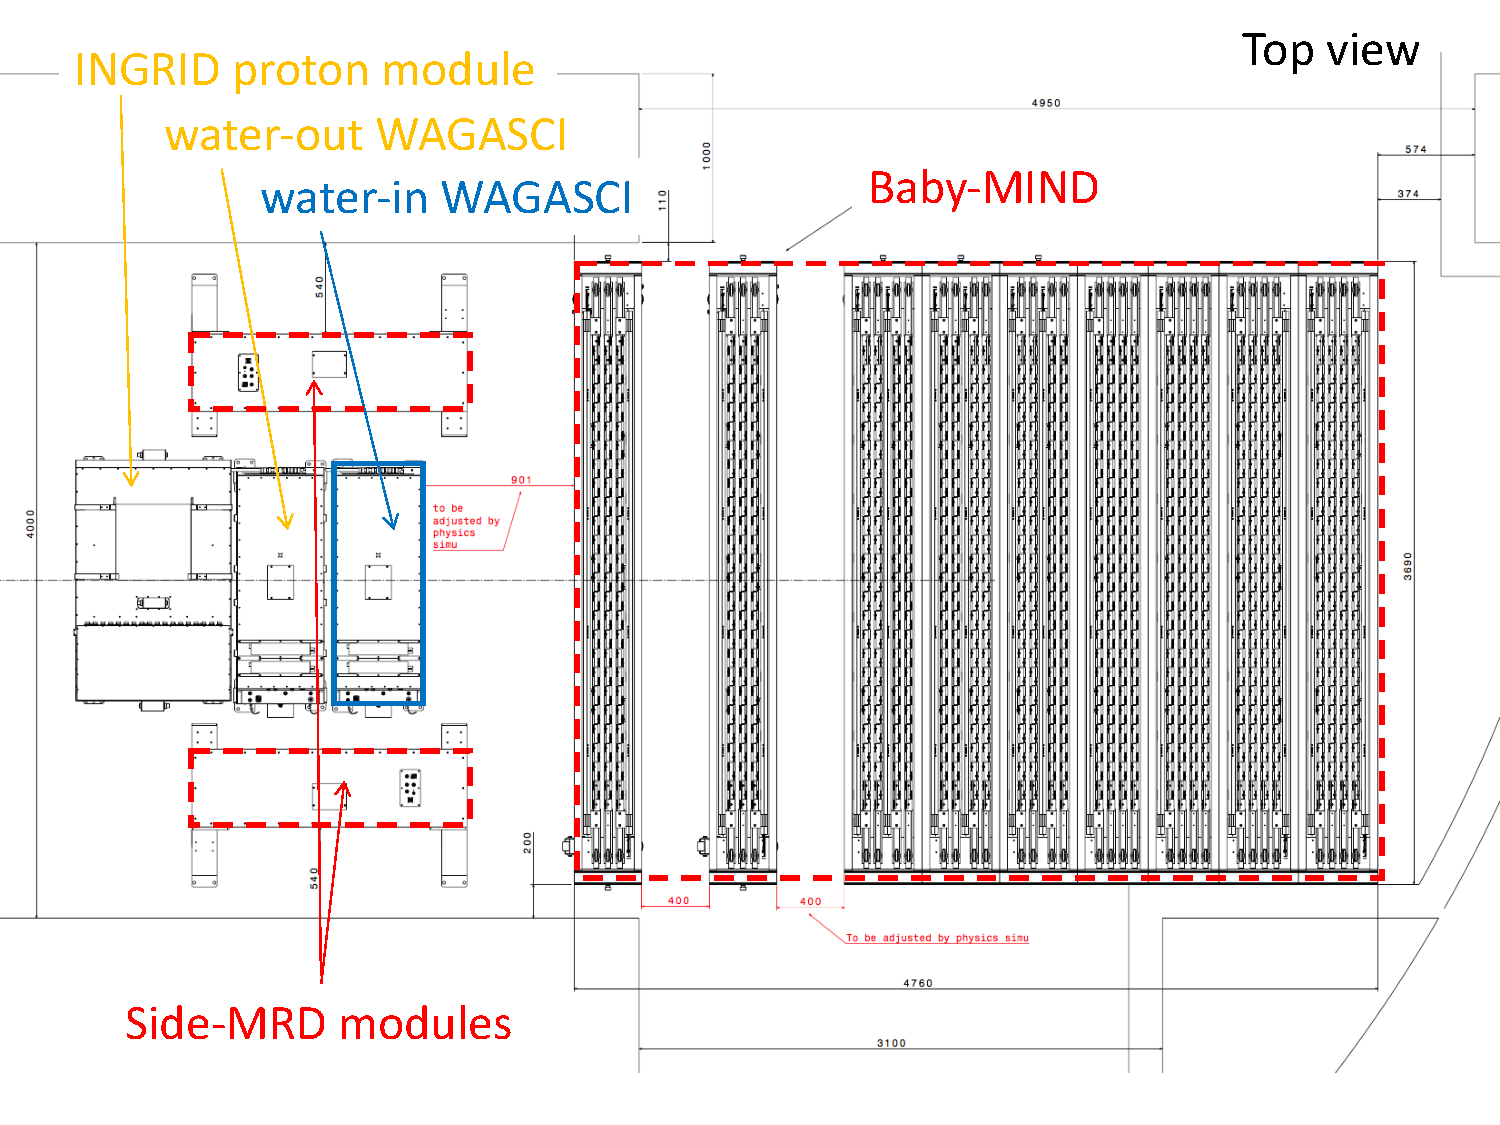
\includegraphics[width=0.8\linewidth]{fig/wagasci_smrd_babymind_topview.pdf}
% \includegraphics[width=0.8\linewidth]{fig/all_detector2.pdf}
\end{center}
\caption{
Top view of entire sets of detectors.
}
\label{fig:all_detector_topview}
\end{figure}


T2K adopted the off-axis beam method, in which
the neutrino beam is intentionally directed 2.5 degrees away from SK producing a narrow band $\nu_{\mu}$ beam.
The off-axis near detector, ND280, is installed towards the SK direction in the B1 floor of the near detector hall of the J-PARC neutrino beam-line.
We propose to install our detector in the B2 floor of the near detector hall, 
where the off-axis angle is similar but slightly different: 1.5 degree.
The candidate detector position in the B2 floor is shown in Fig. \ref{fig:location}.
The expected neutrino energy spectrum at the candidate position is shown in Fig. \ref{fig:b2flux}.

\begin{figure}[tbhp]
\begin{center}
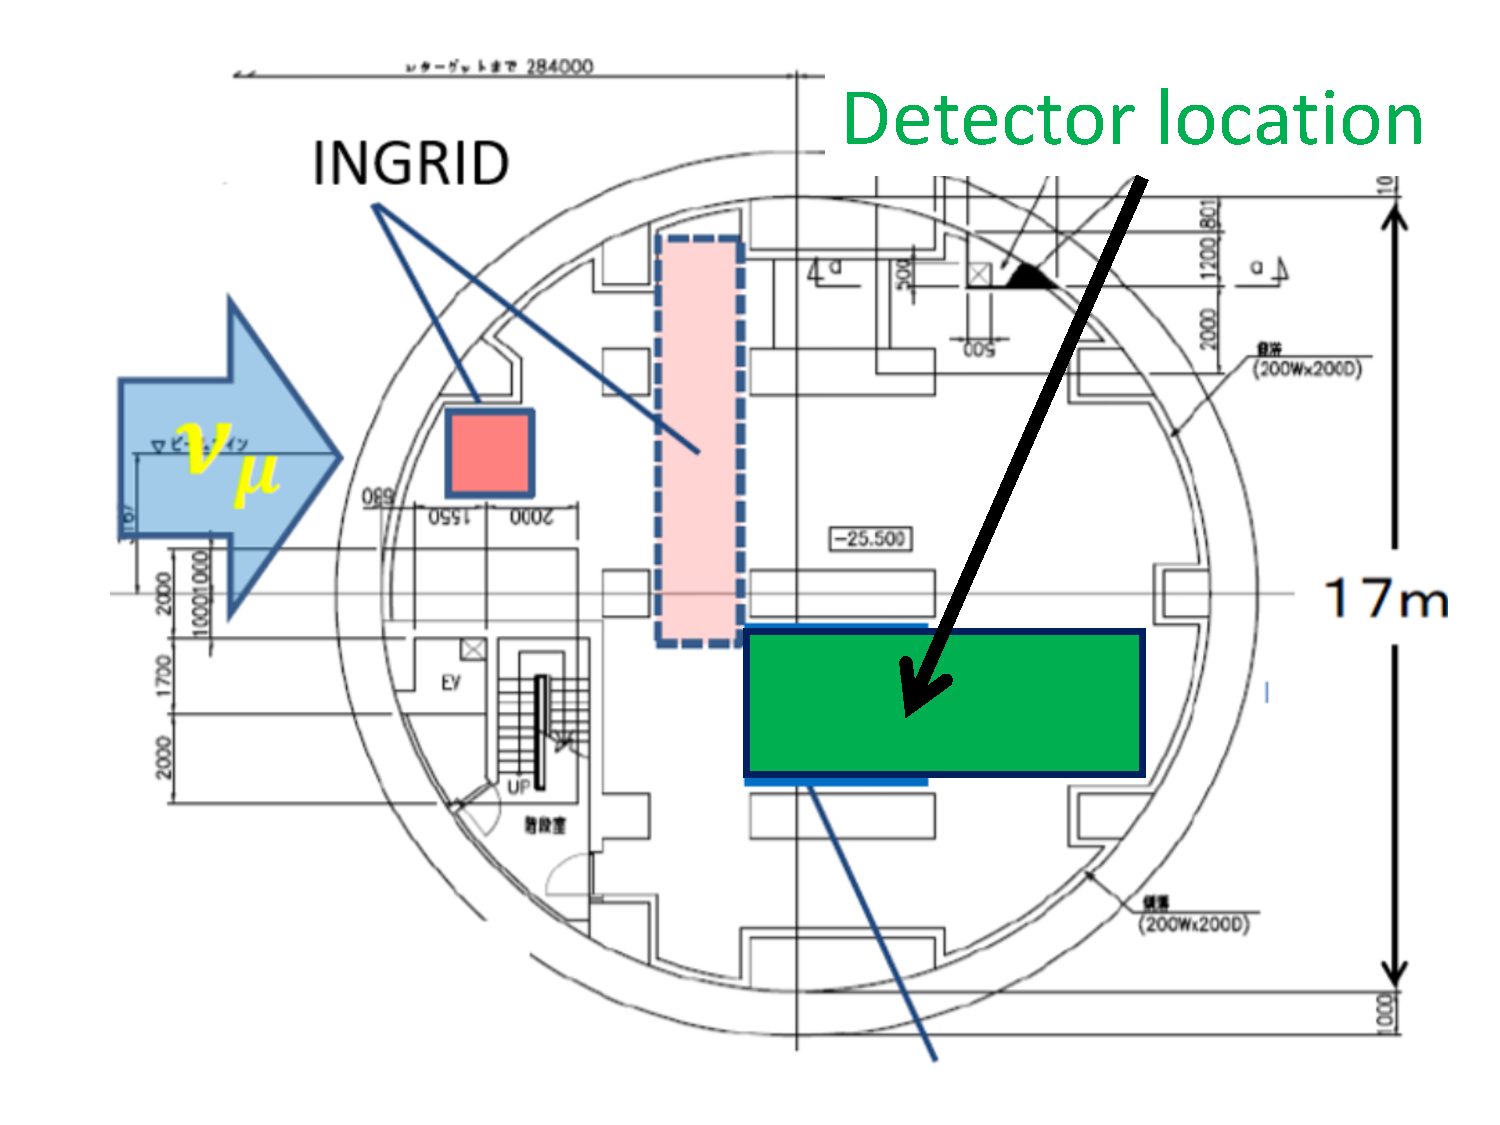
\includegraphics[width=0.7\linewidth]{fig/detector_position_b2.pdf}
% 
\includegraphics[width=0.6\linewidth]{fig/tmp.pdf}
\end{center}
\caption{
Candidate detector position in the B2 floor of the near detector hall.
}
\label{fig:location}
\end{figure}

\begin{figure}[tbhp]
\begin{center}
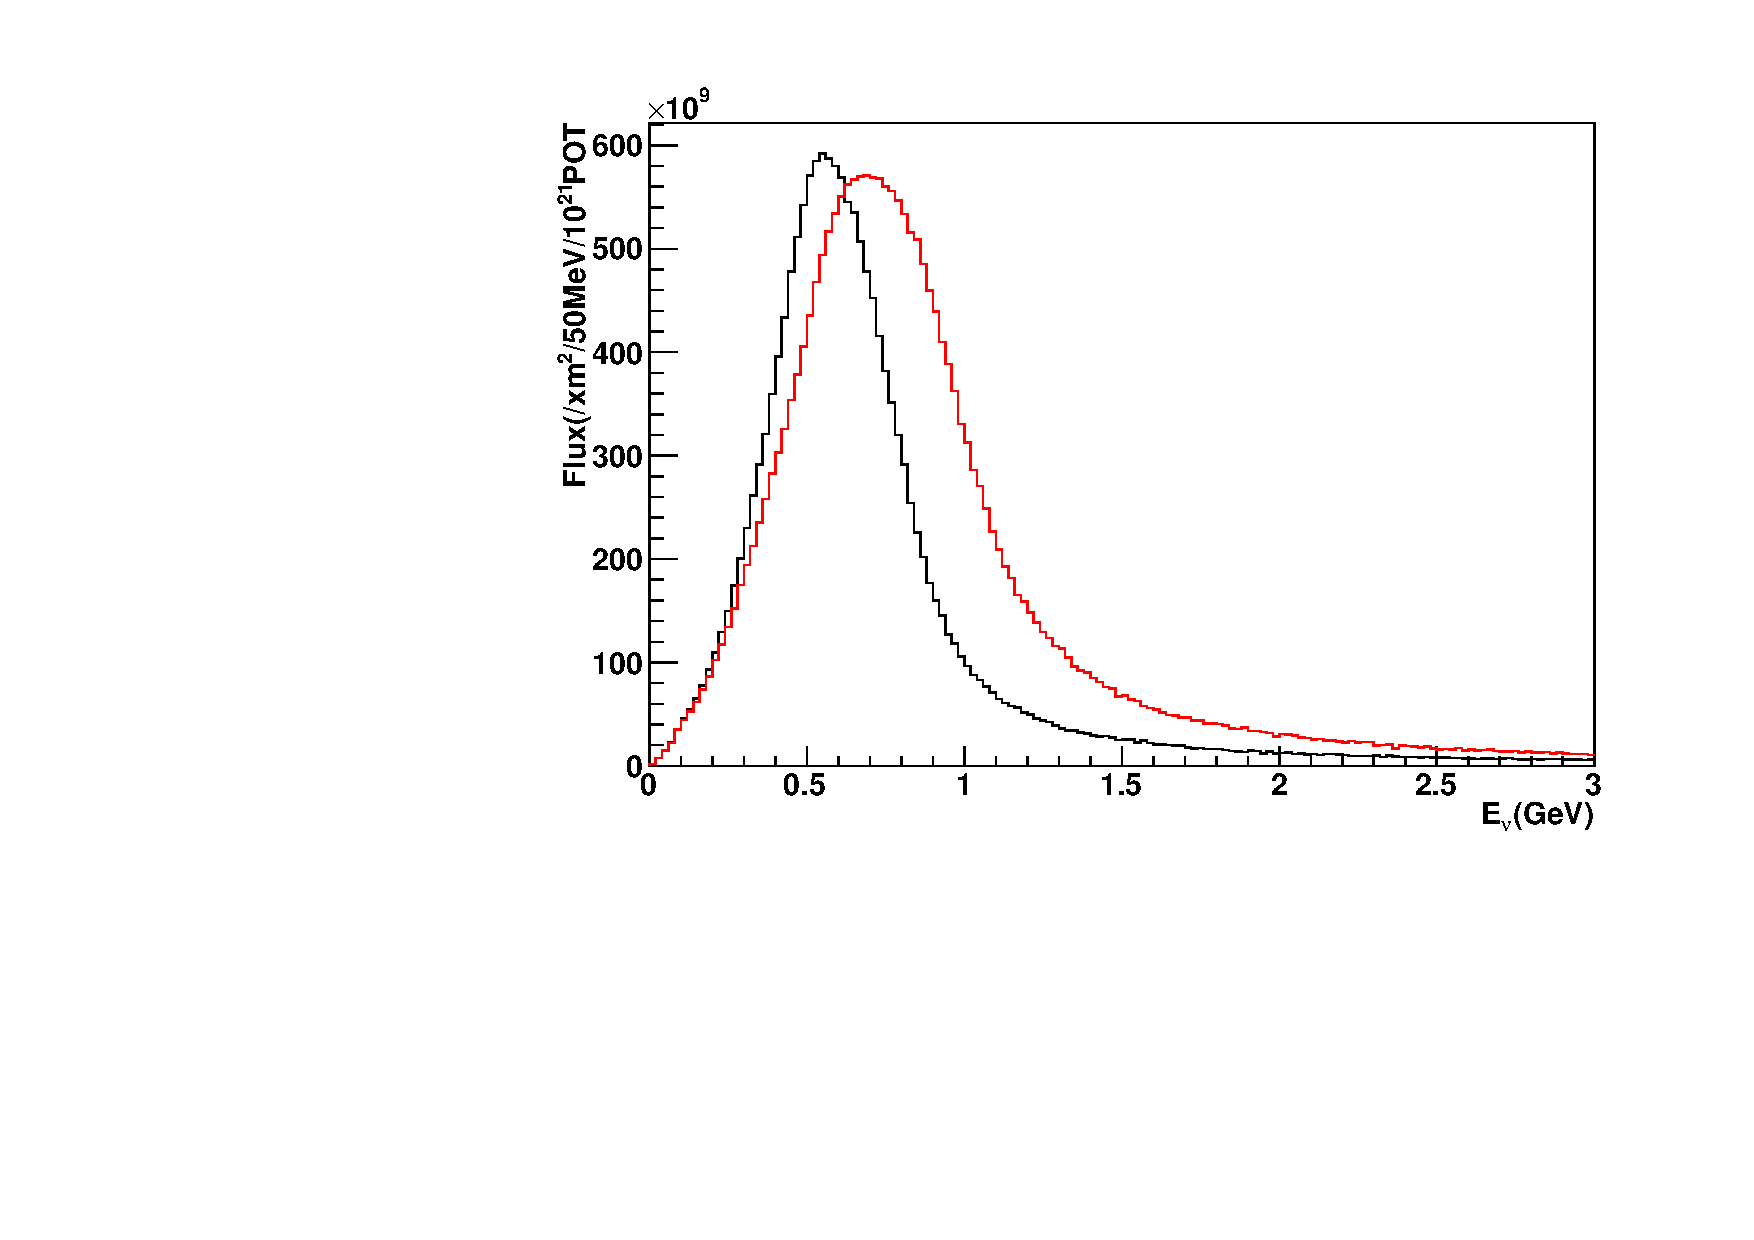
\includegraphics[width=0.4\linewidth, angle=270]{fig/b2_nd280_fluxes.pdf}
\end{center}
\caption{
Neutrino energy spectrum at the candidate detector position(red, off-axis 1.5 degree).
The spectrum at the ND280 site (black, off-axis 2.5 degree) is also shown.
}
\label{fig:b2flux}
\end{figure}


\subsection{Wagasci modules}
\subsubsection{Main detector}
The WAGASCI modules are mainly composed of 1280 plastic scintillator bars and a surrounding stainless steel tank as shown in Fig. \ref{fig:3dgrid_wagascimod}.
The total number of channels in one Wagasci module is 1280.
The stainless steel tank is constructed by welding stainless steel plates, is sized as 46$\times$125$\times$125 cm$^{3}$, and weighs 0.5 ton. 
%The plastic scintillator bars form a three-dimensional grid structure with 5$\times$5$\times$2.5 cm$^{3}$ cells. 


One Wagasci module consists of 16 scintillator tracking planes, where each plane is an array of 80 scintillator bars fixed with ABS frames.
The 40 bars, called parallel scintillators, are placed perpendicularly to the beam, and the other 40 bars, called grid scintillators, are placed in parallel to the beam with grid structure in the tracking plane as shown in Fig. \ref{fig:3dgrid_wagascimod}.
Thanks to the 3 D grid-like structure of the scintillator bars, 
the Wagasci module has $4\pi$ angular acceptance for charged particles.

\begin{figure}[tbhp]
  \begin{center}
   \begin{subfigure}{0.48\textwidth}
     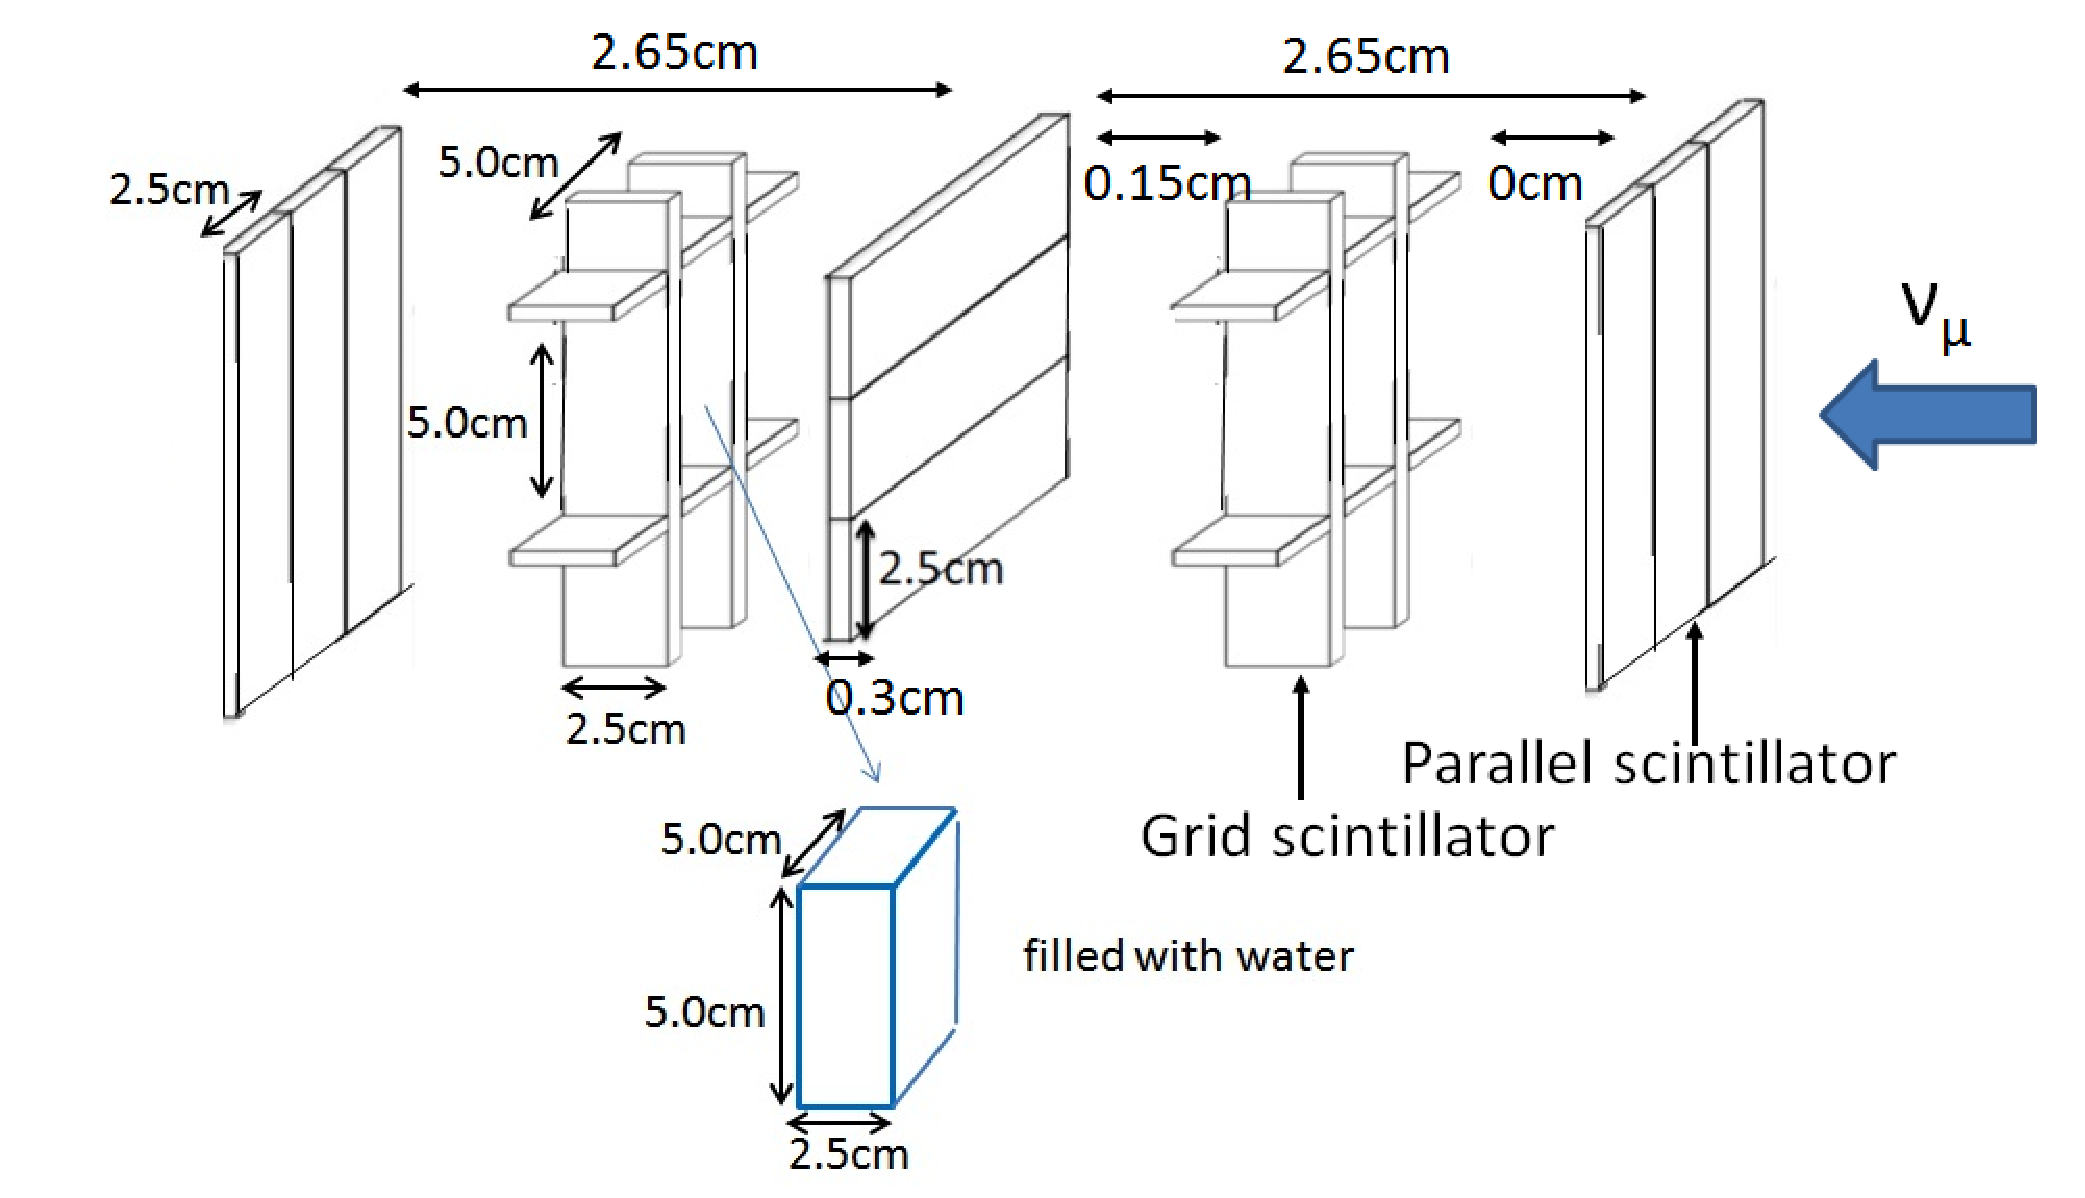
\includegraphics[width=\linewidth]{fig/3d_grid_structure.pdf}
    \end{subfigure}
  \begin{subfigure}{0.48\textwidth}
      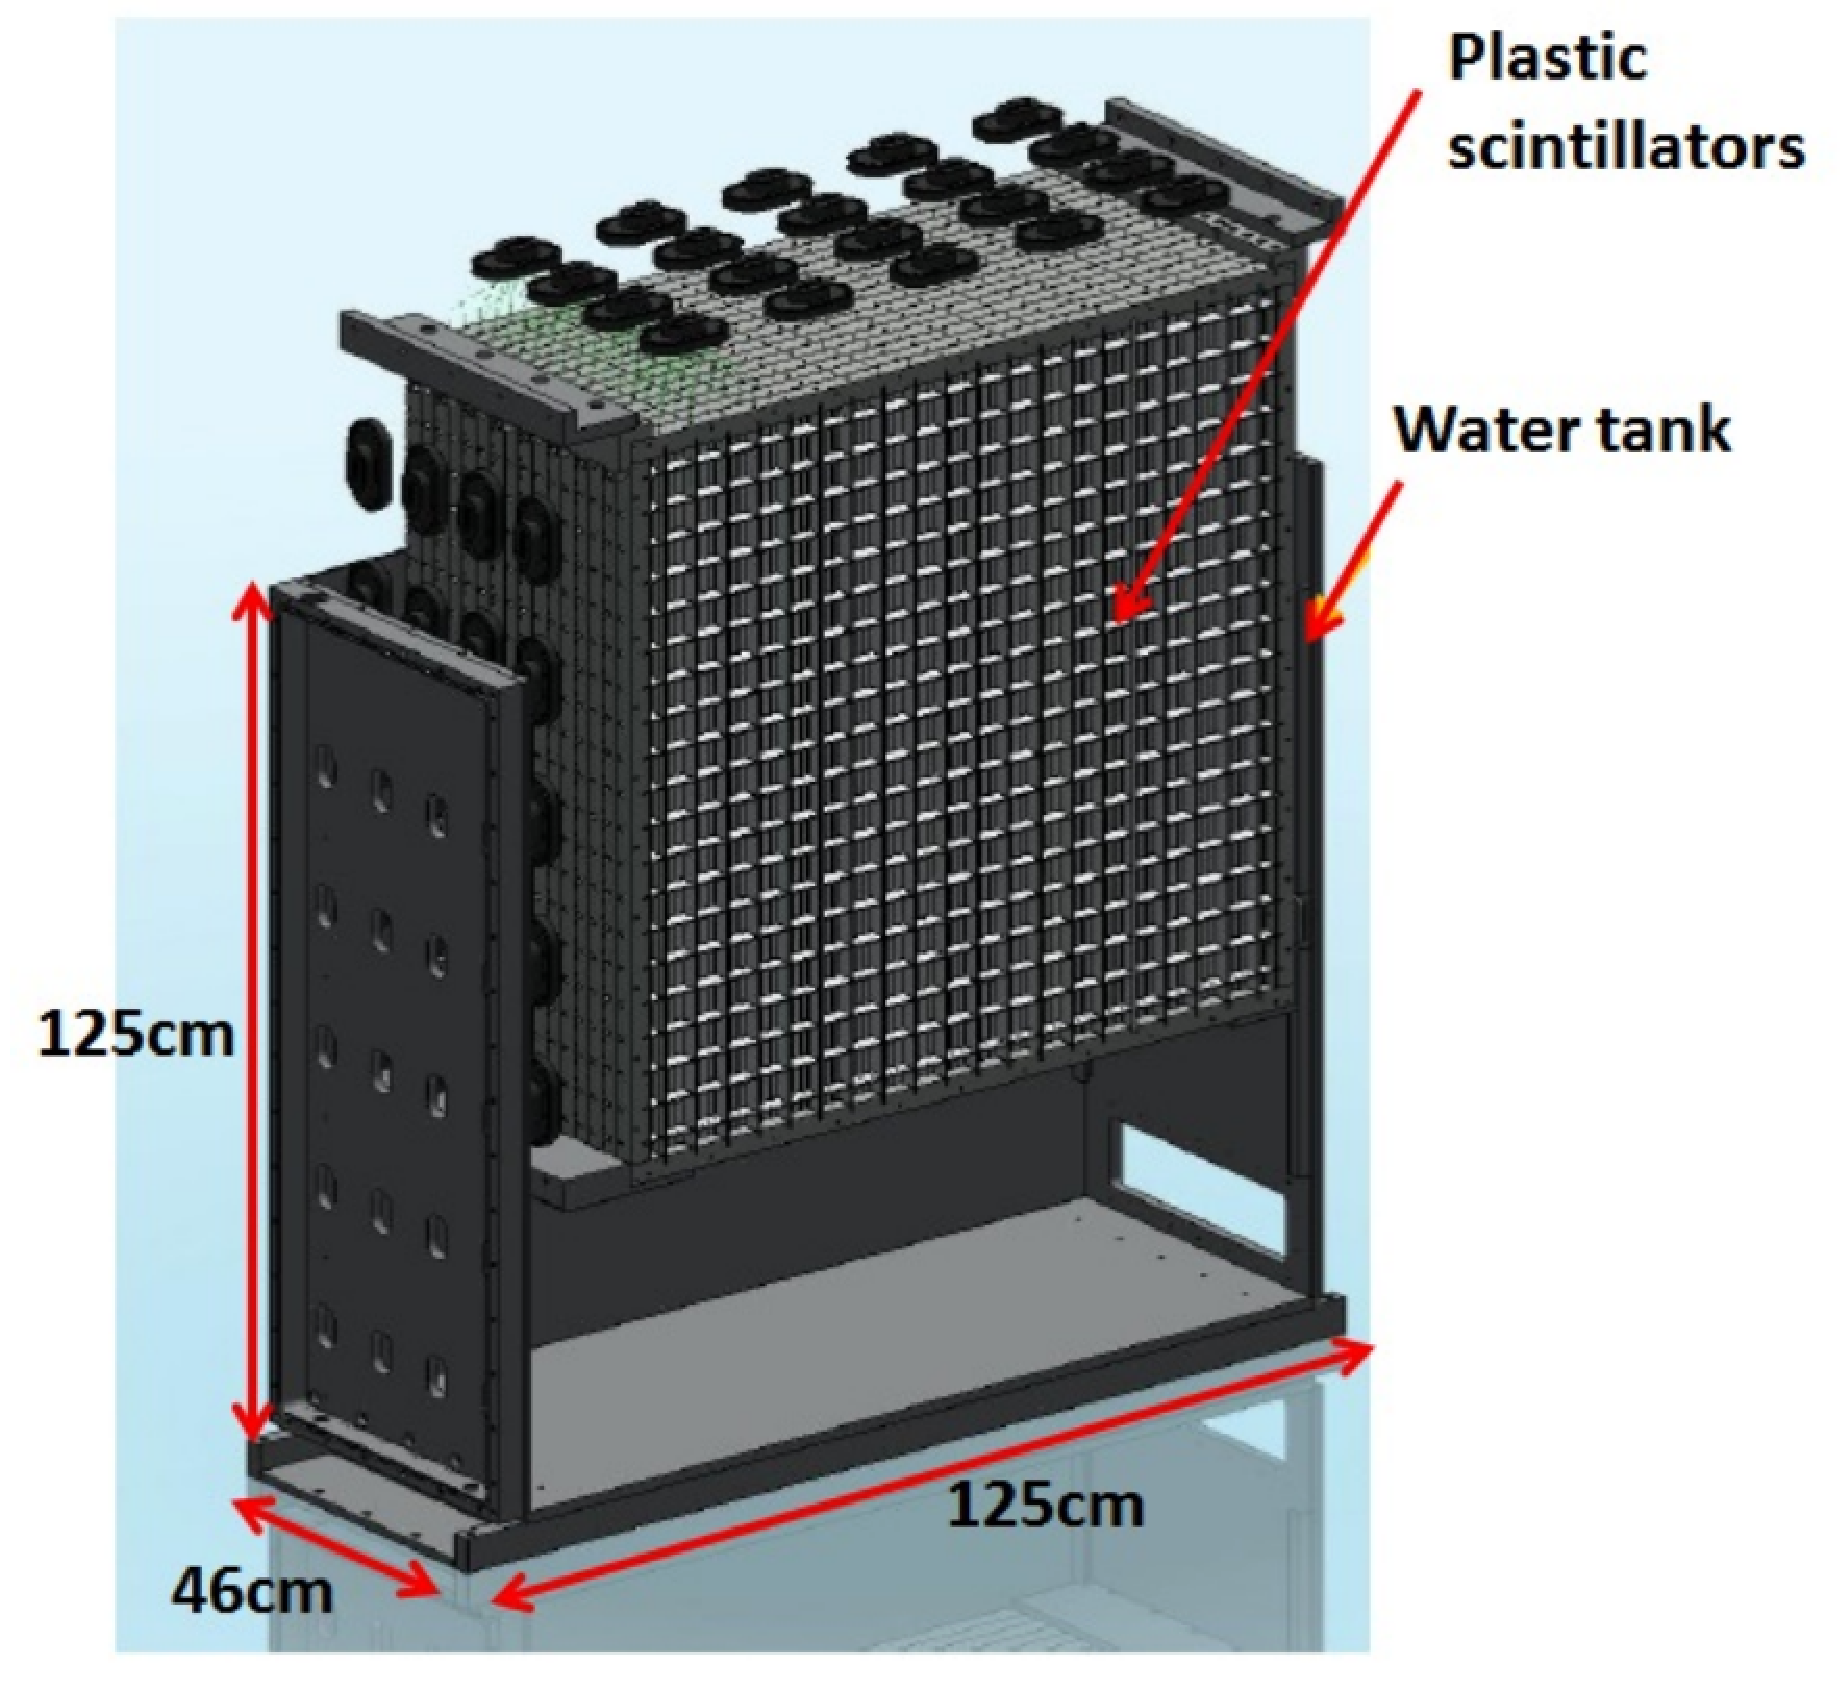
\includegraphics[width=\linewidth]{fig/wagasci_mod.pdf}
    \end{subfigure}    
    \end{center}
  \caption{Schematic views of 3D grid-like structure of plastic scintillator bars (left) and Wagasci module (right).}
\label{fig:3dgrid_wagascimod}
\end{figure}


Thin plastic scintillator bars produced at Fermilab by extrusion method, mainly consists of polystyrene and are surrounded by thin reflector including TiO$^{2}$ (3 mm in thickness) are used for the Wagasci modules to reduce the mass ratio of scintillator bars to water,
because neutrino interactions in the scintillator bars are a background for the cross section measurements on H$_{2}$O.
Each scintillator bar is sized as 1020$\times$25$\times$3 mm$^{3}$ including the reflector part, and 
half of all the scintillator bars have 5-cm-interval slits to form the grid structure (Figure \ref{fig:wagasci_scinti_geometry} ). 

\begin{figure}[tbh]
\begin{center}
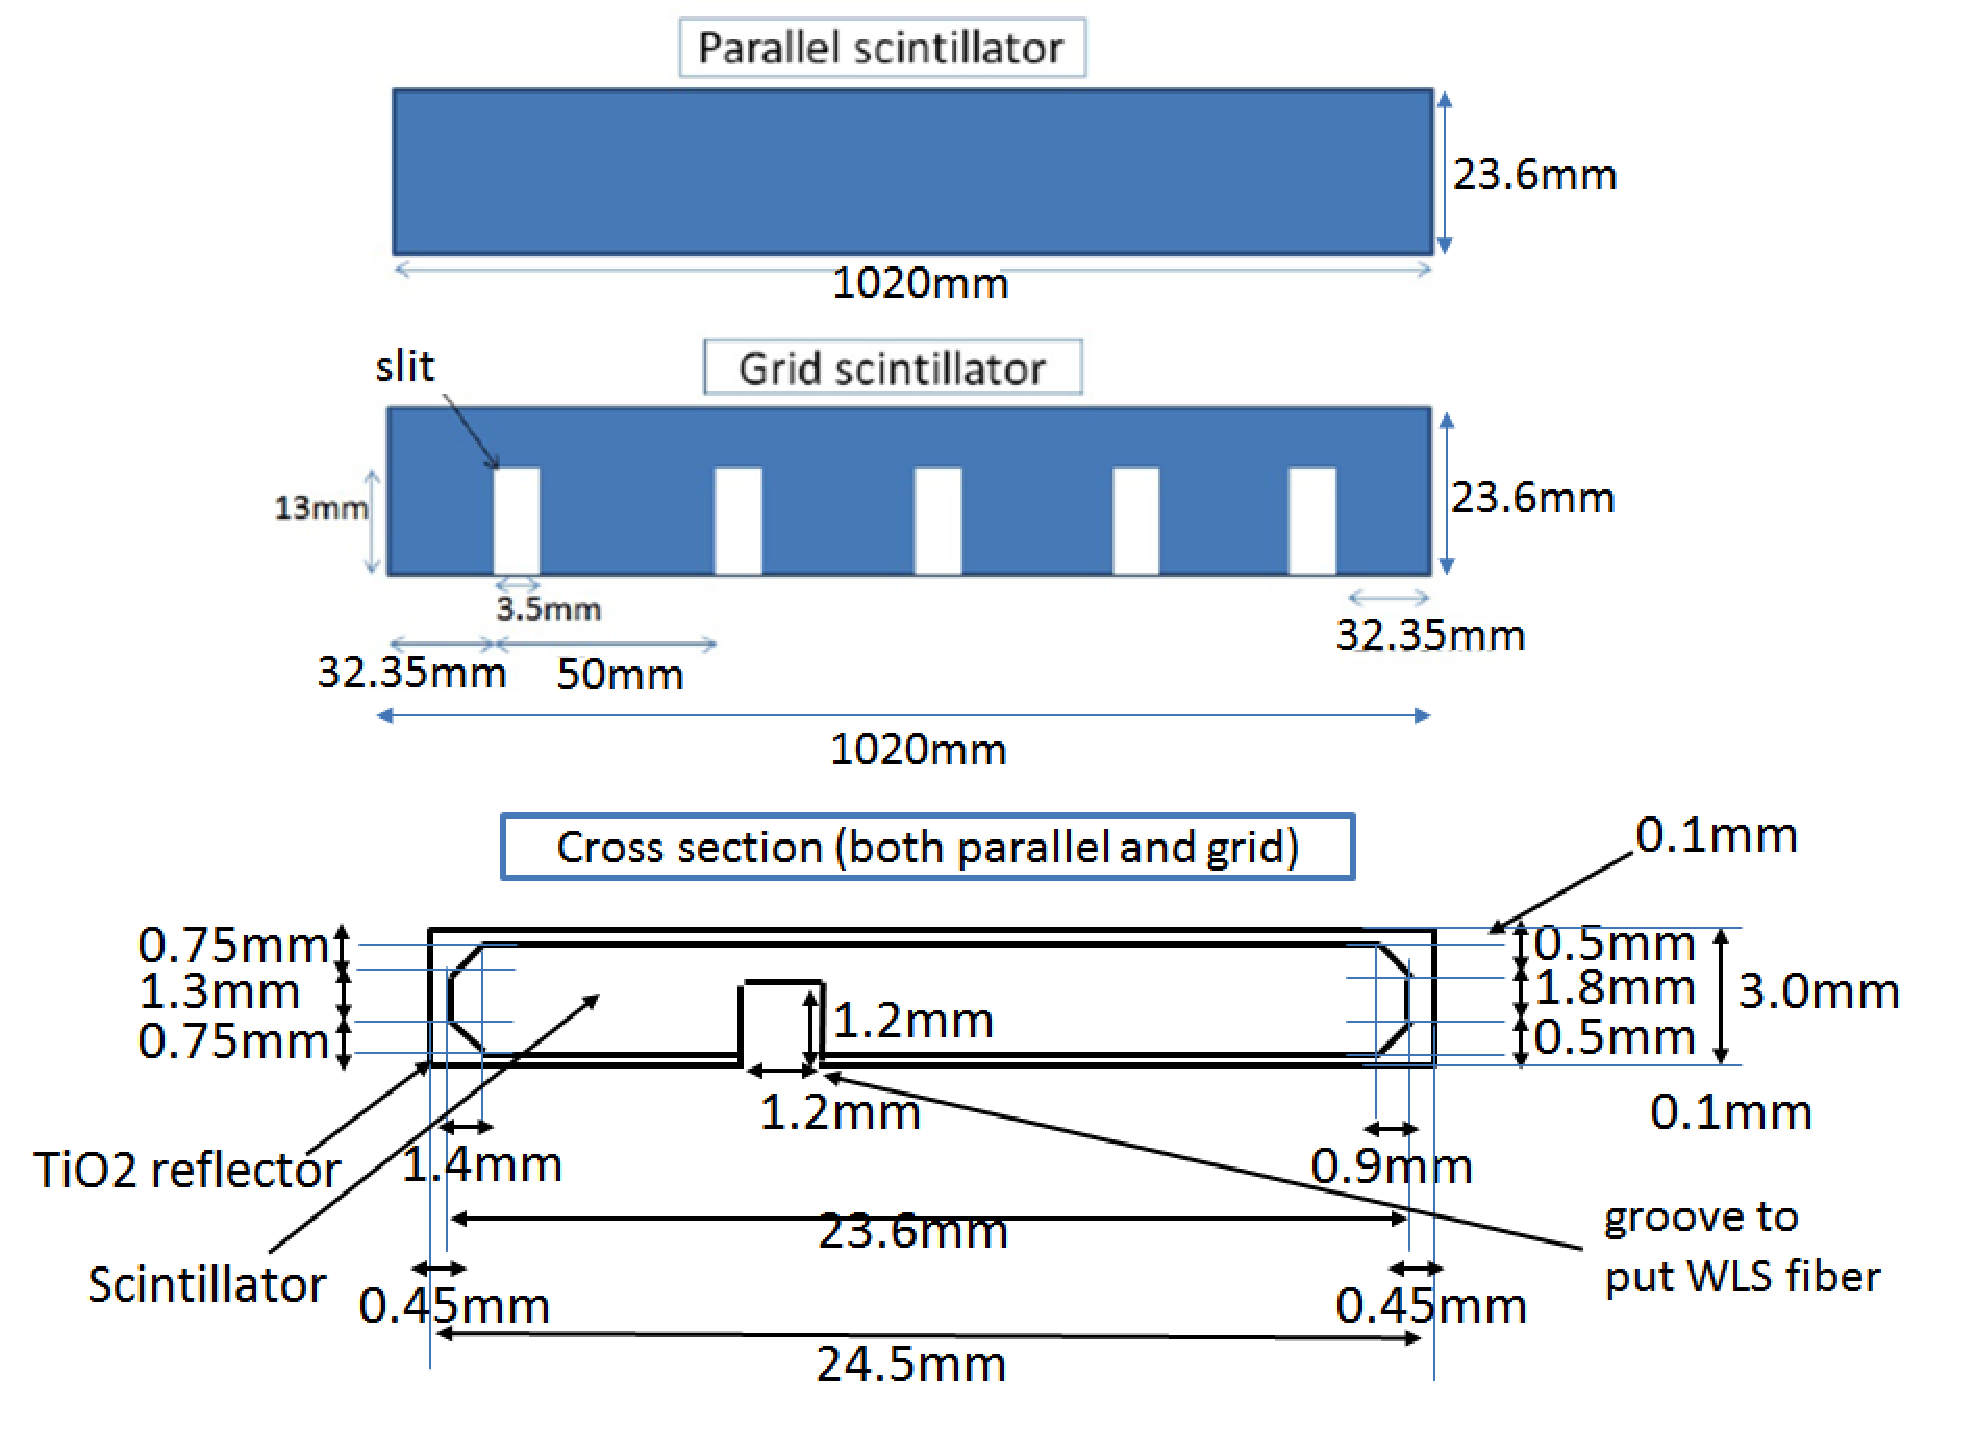
\includegraphics[width=0.8\linewidth]{fig/wagasci_scinti_geometry.pdf}
% 
\includegraphics[width=0.6\linewidth]{fig/tmp.pdf}
\end{center}
\caption{
Geometry of scintillators used for Wagasci modules.
}
\label{fig:wagasci_scinti_geometry}
\end{figure}


We will have two types of the Wagasci modules, a water-in module and a water-out module.
The water-in Wagasci module has water in spaces of the grid structure.
The total water mass serving as neutrino targets in the fiducial volume of the module is 188 kg,
and the mass ratio of scintillator bars to water is 80 \%.
The water-out Wagasci module doesn't have water inside the detector.
The total CH mass serving as neutrino target in the fiducial volume of the module is 47 kg,
and the mass fraction of scintillator bars is 100 \%.


Scintillation light is collected by wave length shifting fibers, Y-11 (non-S type  with a diameter of 1.0 mm produced by Kuraray. 
A fiber is glued by optical cement in a groove on surface of a scintillator bar. 
32 fibers are gathered together by a fiber bundle at edge of the module, and lead scintillation light to a 32-channel arrayed MPPC.
Since crosstalk of light yield due to reflection on the inner surface of each cell has been observed, all the scintillator bars are painted black by aqueous color spray.
It is confirmed by measurements with cosmic rays that black painting on the surface of the scintillator bars suppresses this crosstalk so that no significant crosstalk effect is observed within uncertainty.



32-channel arrayed MPPCs, as shown in the Fig. \ref{fig:wagasci_mppc}, are used for the modules.
The surface of the fiber bundle is polished and directly attached onto the 32-channel arrayed MPPCs. The positions of 32 fibers on the bundle are aligned to fit the channels of MPPCs.
The MPPC is a product of Hamamatsu Photonics, S13660(ES1), with suppressed noise rate of $\sim$6 kHz per channel at 0.5 p.e. threshold.
For each MPPC channel, 716 pixels of APD are aligned in a shape of circle.

\begin{figure}[tbhp]
  \begin{center}
   \begin{subfigure}{0.48\textwidth}
     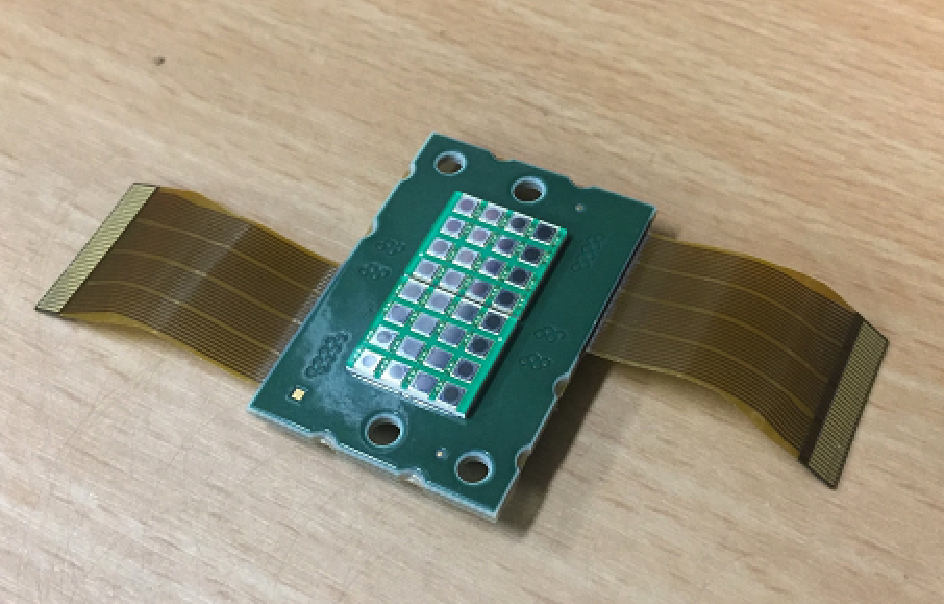
\includegraphics[width=\linewidth]{fig/32ch_array_mppc.pdf}
    \end{subfigure}
  \begin{subfigure}{0.38\textwidth}
      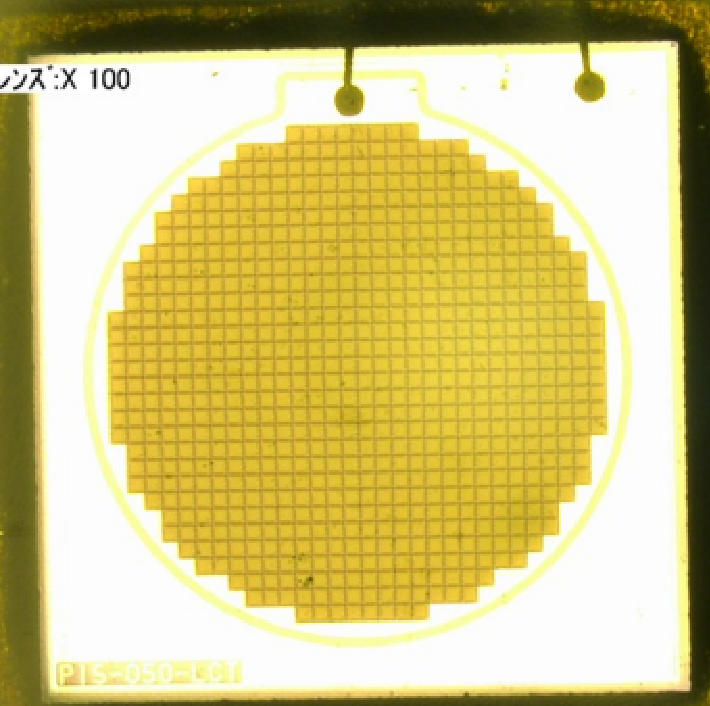
\includegraphics[width=\linewidth]{fig/enlarge_32ch_array_mppc.pdf}
    \end{subfigure}    
    \end{center}
  \caption{32-channel arrayed MPPC (left) and an enlarged view of one MPPC channel (right).}
\label{fig:wagasci_mppc}
\end{figure}


\subsubsection{Electronics}
As front-end electronics of this detector, a Silicon PM Integrated Read-Out Chip (SPIROC) \cite{spiroc} is adopted.
SPIROC is a 36-channel auto-triggered front-end ASIC, and is produced by OMEGA/ IN2P3. 
It not only contains an analog signal processing part such as amplification and shaping of the waveform, but contains a digital signal processing parts such as auto-trigger and timing measurement.
Charge of MPPC signal is sampled by track-and-hold circuit.
A Front-end electronics board, Active Sensor Unit (ASU), has been developed with the SPIROC2D chip, which is the latest version of SPIROC. 
Each readout board is designed to control a 32-channel arrayed MPPC, and 40 of the ASU boards are aligned on the module surface. 
The data acquisition system used for this detector, including back-end boards, has been developed for prototypes of ultra-granular calorimeters for the International Linear Collider (ILC) \cite{cal_ilc}, and independent of the T2K DAQ system.
To synchronize the DAQ system to J- PARC neutrino beam, pre-beam trigger and beam trigger are sent to the clock control card.
The beam trigger signals are converted from optical signals to NIM signals at NIM module on the B2 floor.
In addition, the information of spill number are delivered with 16-bit ECL level signals, and converted to an Ethernet frame by an FPGA evaluation board to be directly sent to the DAQ PC.
The electronics readout scheme is shown in Fig. \ref{fig:wagasci_elec_scheme}.
% The event of the WAGASCI module will be off-line matched with those of INGRID placed at the B2 floor and Proton Module by using the spill number information.

\begin{figure}[tbh]
\begin{center}
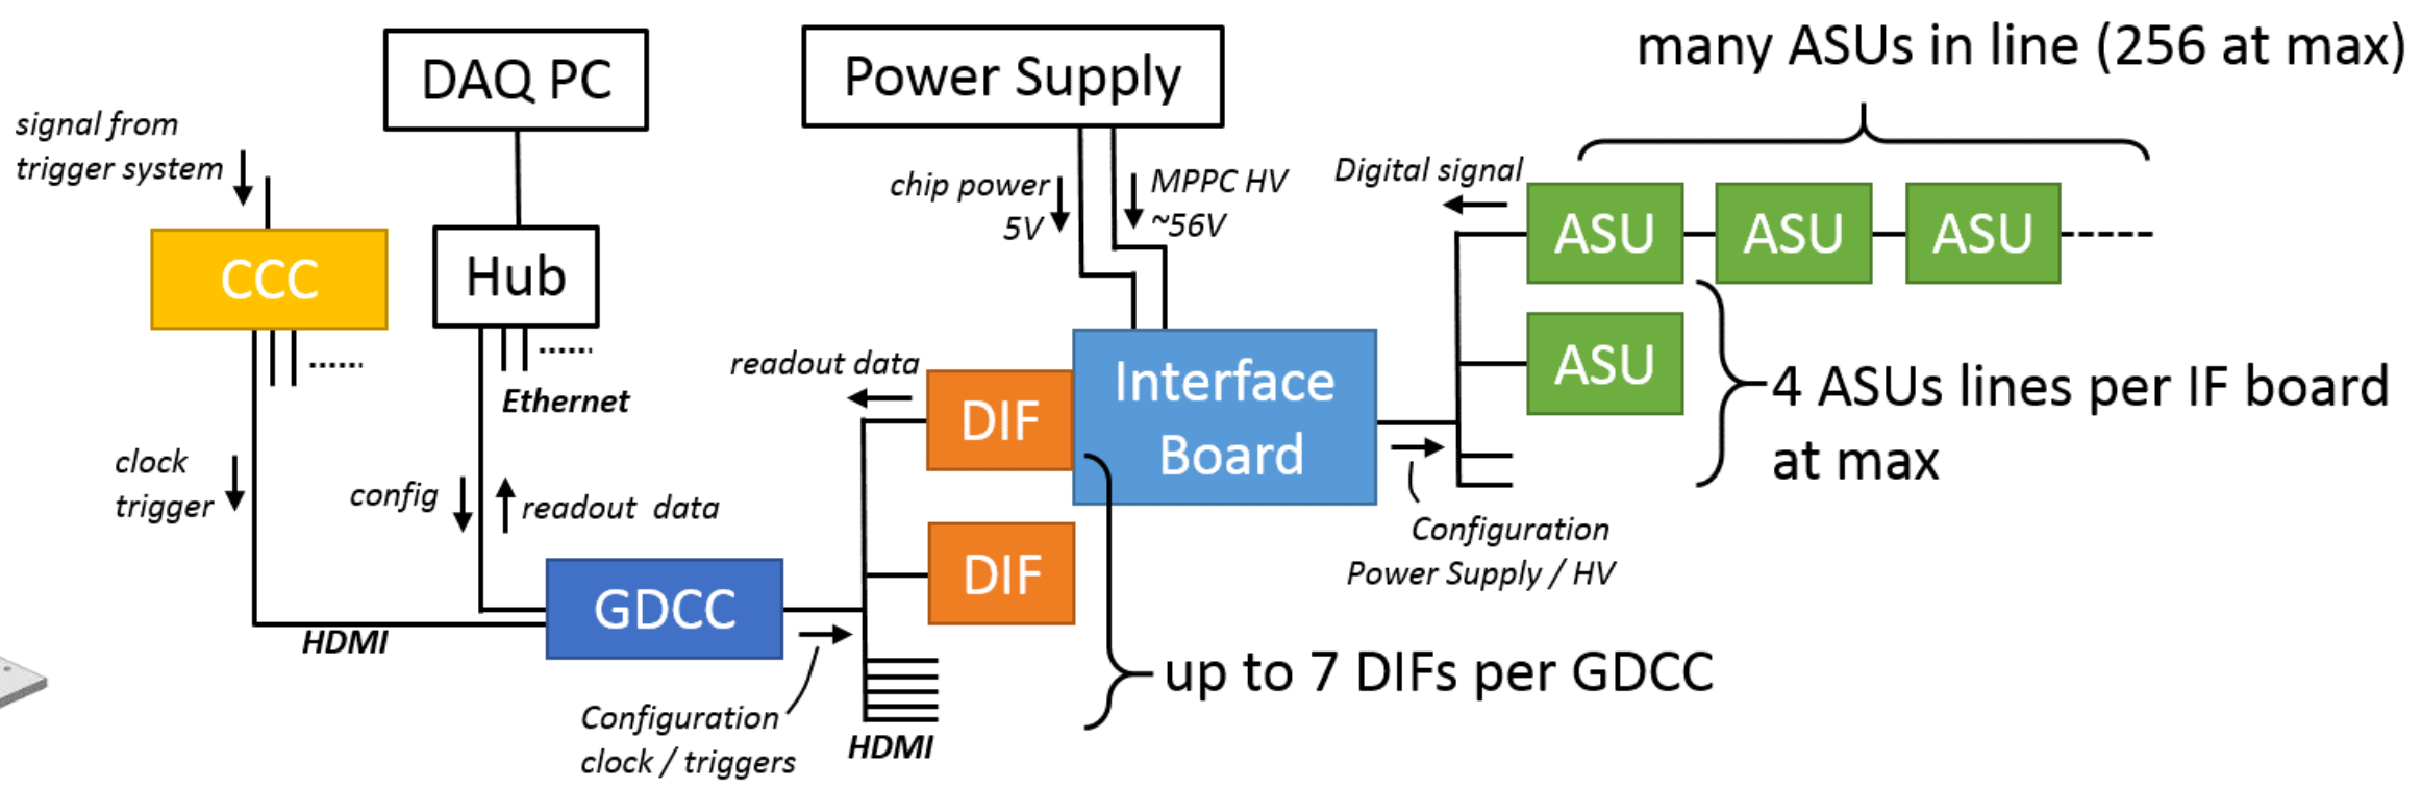
\includegraphics[width=1.0\linewidth]{fig/wagasci_elec_scheme.pdf}
% 
\includegraphics[width=0.6\linewidth]{fig/tmp.pdf}
\end{center}
\caption{
Wagasci electronics readout scheme.
}
\label{fig:wagasci_elec_scheme}
\end{figure}


\subsubsection{Water system}
Pure water is filled to the water tank of the water-in Wagasci module as follows.
First, the water storage tank located at the B2 floor of the NM pit is filled with water delivered from a water tap on the ground level through a long hose. 
Second, the water is pumped to the other water storage tank though a water filler to produce pure water.
Third, a compound preservative called Germall plus, which is the same preservative used in one of the sub-detectors of T2K ND280, FGD2, is put into the water to keep water from being bad.
Then, the water is poured to the water-in Wagasci module, and it is kept in the module during the neutrino beam operation and not to be circulated.


\subsection{INGRID Proton module}
INGRID Proton module is a neutrino detectors of the T2K experiment.
It is a fully-active tracking detector which consists of only scintillator strips. 
The purpose of this Proton Module is to separate the neutrino interaction types by detecting the protons and pions together with the muons from the neutrino interactions, and to measure the neutrino cross section for each interaction type.
It consists of 36 tracking planes surrounded by veto planes (Figure \ref{fig:proton_module}), where each tracking plane is an array of two types of scintillator strips. 
The 16 strips in the inner region have dimensions of 2.5cm$\times$1.3cm$\times$120cm, while the 16 strips in the outer region have dimensions of 5cm$\times$1cm$\times$120cm, making a plane of 120$\times$120cm$^{2}$ in the horizontal and vertical directions.
The former is the scintillator produced for the K2K SciBar detector \cite{scibar} and the latter was produced for INGRID.
The tracking planes are placed perpendicular to the beam axis at 23mm intervals.
Since the strips are aligned in one direction, each tracking plane is sensitive to either the horizontal or vertical position of the tracks.
The tracking planes are therefore placed alternating in the horizontal and vertical directions so that three-dimensional tracks can be reconstructed.
The tracking planes also serve as the neutrino interaction target.
As with the Wagasci modules, scintillation light is read out by a WLS fiber and MPPC.


It was installed at the neutrino beam axis on the SS floor of the T2K near detector hall in 2010, and had been used for neutrino cross section measurements.
In August 2017, it was moved to the B2 floor of the T2K near detector hall by J-PARC T59 after getting the approval from T2K to use them.
J-PARC T59 is performing a  neutrino beam measurement using the detector from October 2017, and the measurement  will continue until May 2018 as we will discuss in Sec. \ref{sec:t59status}.

\begin{figure}[tbh]
\begin{center}
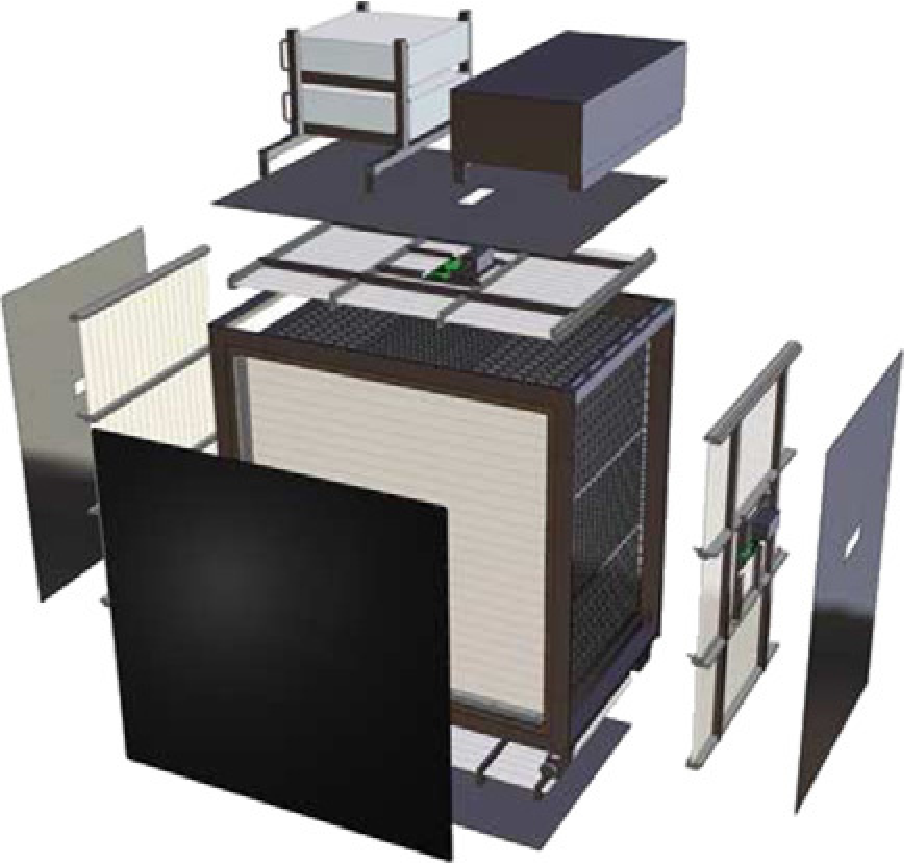
\includegraphics[width=0.6\linewidth]{fig/proton_module.pdf}
\end{center}
\caption{
Schematic view of INGRID Proton module.
}
\label{fig:proton_module}
\end{figure}


We will operate the INGRID Proton module using the T2K near detector electronics/DAQ system in the same way as J-PARC T59.
A proposal to use the module and its electronics for our project will be submitted to the T2K collaboration.


\subsection{Baby MIND}
The Baby MIND is the downstream Muon Range Detector.
It also works as a magnet and provides the charge identification capability
as well as magnetic momentum measurement for high energy muons.

The Baby MIND collaboration \footnote{Contact person: E. Noah, Spokesperson: A. Blondel, Deputy spokesperson: Y. Kudenko} submitted a proposal to the SPSC at CERN, SPSC-P-353.
The project was approved by the CERN research board as Neutrino Platform project NP05 and constructed.
The detector consists of 33 magnet modules, each 3500 mm $\times$ 2000 mm$ \times$ 50 mm (30 mm steel) with a mass of approximately 2 tonnes. Of these magnet modules, 18 are instrumented with plastic scintillator modules. 

%The main Baby MIND systems are the magnet, scintillator and electronics modules \cite{Noah:EPS2017}.
%A total of 3,996 silicon photomultipliers are read out by custom electronics Front End Boards that can process up to 96 channels each, sending charge and timing information of hits in the detector to dedicated data acquisition computers.

%One challenge to be addressed by the Baby MIND collaboration is that of obtaining high charge identification efficiencies for $\mu^+/\mu^-$ down to 500 MeV/c and below. Magnetized iron neutrino detectors are limited by multiple scattering in the iron, and their use is overlooked for applications requiring good charge ID efficiencies below 1 GeV/c. By optimizing the distance between the first magnet modules, rendered possible by the magnet design, our simulations show improved charge identification efficiencies down to 400 MeV/c.


\subsubsection{Magnet modules}
Traditional layouts for magnetized iron neutrino detectors (e.g. MINOS) tend to be monolithic blocks
with a unique pitch between consecutive steel segments and large conductor coils threaded around the whole magnet volume.
The Baby MIND detector, like traditional designs, is built from sheets of iron interleaved with scintillator detector modules.
However Baby MIND is novel in that the iron segments are all individually magnetized as shown in Figure ~\ref{fig:BM_winding}, allowing for far greater flexibility in the setting of the pitch between segments, and in the allowable geometries that these detectors can take.


The key design outcome is a highly optimized magnetic field map. A double-slit configuration for coil winding was adopted to increase the area over which the magnetic flux lines are homogeneous in $B_x$ across the central tracking region. Simulations show the magnet field map to be very uniform over this central tracking region covering an area of $2800\times2000$ mm$^2$, Figure~\ref{magnet-cross-sections}. The $B_x$ component dominates in this region, with negligible $B_y$ and $B_z$. This was confirmed by measuring the field with 9 pick-up coils wound around the first module. Subsequent modules were equipped with one pick-up coil. Test results on the 33 modules show all achieve the required field of 1.5 T for a current of 140 A, with a total power consumption of 11.5 kW. The polarity of the field map shown in Figure~\ref{magnet-cross-sections} (middle) can be reversed by changing the power supply configuration.
\insertgraph{0.5}{magnet_assembly_zone.pdf}{Magnet assembly zone at CERN. }{fig:BM_winding}
\inserttwographs{0.5}{b-field-1500a-280cm-coil.pdf}{0.4}{magnetic_field_measurements_per_batch.pdf}{Left) Magnetic field map with a coil along 2800 mm of the length of the plate. Right) Measured B field for 33 modules.}{magnet-cross-sections}

\subsubsection{Scintillator modules}
Each of the 18 scintillator modules is constructed from 2 planes of horizontal counters (95 counters in total) and 2 planes of vertical counters (16 counters in total) \cite{Antonova:2017tuf}, arranged with an overlap between planes to achieve close to 100\% hit efficiency for minimum ionizing muons. The arrangement of planes within a module is vertical-horizontal-horizontal-vertical. This arrangement was the result of an assembly approach whereby each plane was built from 2 half-planes, with each half plane consisting of a horizontal plane and a vertical plane.
The scintillator bars are held in place using structural ladders that align and maintain the counters, Figure~\ref{proto-module-ladders}. No glue is used in the process, so counters can be replaced. Aluminum sheets front and back provide light tightness.

\insertthreegraphs{0.32}{top_front_module.pdf}{0.32}{bottom_front_module.pdf}{0.32}{rear-half-module.pdf} {Scintillator modules assembly. Left) top of front half-module showing vertical counters, and the spacer-ladders that set the pitch between horizontal counters and hold them in place. Middle) rear half-module showing horizontal counters on their ladders. Right) Assembled rear half-module, the front half-module can be seen in the background.}{proto-module-ladders}

The plastic scintillator counters were made from 220 mm-wide slabs, consisting of extruded polystyrene doped with 1.5\% paraterphenyl (PTP) and 0.01\% POPOP. They were cut to size then covered with a 30-100 $\mu$m thick diffuse reflector resulting from etching of the surface with a chemical agent \cite{Kudenko:2001qj, Mineev:2011xp}. The horizontal counter size is $2880 \times 31 \times 7.5 $ mm$^3$, with one groove along the length of the bar in which sits a wavelength shifting fiber from Kuraray. The vertical counter size is $1950 \times 210 \times 7.5 $ mm$^3$, with one U-shaped groove along the bar. On each counter, two custom connectors house silicon photomultipliers, MPPC type S12571-025C from Hamamatsu, either side of the horizontal counter, and both connectors at the top for the vertical counter. This geometrical configuration for vertical counters was chosen for ease of connectivity to the electronics, and maintenance operations.

A total of 1744 horizontal counters and 315 vertical counters (including spares) were produced at the Uniplast company (Vladimir, Russia).

\subsubsection{Electronics}
The Baby MIND electronic readout scheme includes several custom-designed boards \cite{Noah:2016ikh}. The revised version is shown in Figure~\ref{block_diagrams}. At the heart of the system is the electronics Front End Board (FEB), developed by the University of Geneva. The readout system includes two ancillary boards, the Backplane, and the Master Clock Board (MCB) whose development has been managed by INRNE (Bulgarian Academy of Sciences) collaborators.

%One critical element in the photosensor readout path is the cable bundle, a 5 m extension coaxial cable RG174U that connects the photosensor to the FEB. Each bundle connects up to 32 photosensors. The purpose is to decouple the FEBs from the scintillator modules, which improves accessibility to FEBs and their long term maintainability. The module end of the bundle hosts some electronics that manages the application of the high voltage to the SiPMs, enabling faulty SiPMs to be switched off at that level. This feature was added after the summer 2016 beam tests, where a short circuit on a single channel would disable a bank of 96 channels.

\inserttwographs{0.47}{readout_scheme_2.pdf}{0.45}{electronics_connectivity_detailed.pdf}{Left) Baby MIND electronics readout scheme. Right) SiPM-to-FEB connectivity.}{block_diagrams}

The FEBv2 hosts 3 CITIROC chips that can each read in signals from 32 SiPMs \cite{Fleury:2014hfa}.
Each signal input is processed by a high gain (HG), and a separate low gain (LG), signal path.
The outputs from the slow shapers can be sampled using one of two modes: a mode with an externally applied delay, and a peak detector mode. A faster shaper can be switched to either HG or LG paths, followed by discriminators with adjustable thresholds providing 32 individual trigger outputs and one OR32 trigger output. An Altera ARIA5 FPGA on the FEBv2 samples these trigger outputs at 400 MHz, recording rising and falling times for the individual triggers and assigning time stamps to these. 
Time-over-threshold, the difference between falling and rising times, gives some measure of signal amplitude. This is used in addition to charge information and proves useful if there is more than one hit per bar within the $\sim9$ $\mu$s deadtime due to the readout of the multiplexed charge output.
The ARIA5 also manages the digitization of the sampled CITIROC multiplexed HG and LG outputs via a 12-bit 8-ch ADC. 

%The FEBv2 is designed to fit into a slot in a minicrate as shown in Figure \ref{minicrate}. The front face receives the SiPMs cable bundles, the rear end plugs into the backplane. Up to 6 FEBv2 can be housed in each minicrate. Eight minicrates are distributed either side of the Baby MIND.

The internal 400 MHz clock on the FEBv2 can be synchronized to a common 100 MHz clock. The synchronization subsystem combines input signals from the beam line into a digital synchronization signal (SYNC) and produces a common detector clock (CLK) which can eventually be synchronised to an external experiment clock. Both SYNC and CLK signals are distributed to the FEBs. Tests show the FEB-to-FEB CLK(SYNC) delay difference to be 50 ps (70 ps). Signals from the beam line at WAGASCI include two separate timing signals, arriving 100 ms and 30 $\mu$s before the neutrino beam at the near detectors. The spill number is available as a 16-bit signal. 
%\insertthreegraphs{0.31}{FEBv2_horizontal_low_res.jpg}{0.2}{FEB_v2_in_crate_low_res2.jpg}{0.145}{rear_minicrate.jpg}{Left) Second version of the electronics readout Front End Board (FEBv2), received at the University of Geneva in March 2017. Middle) FEBv2 in minicrate. Right) rear of minicrate with 6 FEBs connected through a Backplane PCB on the lower half of the minicrate.}{minicrate}

%Several connection options are possible between the FEBv2 and a DAQ PC. The FEBv2 can be operated as a standalone device, connected directly to a DAQ PC via USB3. This is useful for laboratory measurements on the FEB itself, its maintenance and calibration, and qualification tests on other components such as MPPCs or cable bundles. It is also possible to daisy chain several FEBs via the backplane PCB in experiment data taking mode, with the first FEB in the chain connected directly to the DAQ PC via a USB3 link. In this mode the USB3 bandwidth is shared with the potential 6 FEBs in the chain thanks to a Time Division Multiplexing (TDM) protocol, each FEB having $1/6$th of the data throughput. For enhanced measurements or calibration a dedicated option of the chaining is also possible where 1 single FEB in the chain can use the full bandwidth of the single USB3 connection. The DAQ software is platform independent. The data protocol encodes information such as spill number, FEB ID, hit channel number, time and charge, as well as tags to match the TDM data stream to the correct minicrate slot ID.

\subsubsection{Pefromance check}
All counters were measured at INR Moscow with a cosmic ray setup using the same type S12571-025C MPPCs and CAEN DT5742 digitizer.% \cite{Antonova:2017cdw}.
The average light yield (sum from both ends) was measured to be 37.5 photo-electrons (p.e.) per minimum ionizing particle (MIP) and 65 p.e./MIP for vertical and horizontal counters, respectively. After shipment to CERN, all counters were tested once more individually with an LED test setup \cite{led_test_system}. 0.1\% of counters failed the LED tests and were therefore not used during the assembly of modules. 
The assembly of modules was completed in June 2017, and it was then tested in June and July 2017 at the Proton Synchrotron experimental hall at CERN with a mixed particle beam comprising mostly muons whose momenta could be selected between 0.5 and 5 GeV/c. An event display from the summer 2017 tests is shown in Figure~\ref{beam_vs_cosmic}.
%\inserttwographs{0.45}{baby_mind_wagasci_rough_cad.pdf}{0.50}{baby_mind_layout.pdf}{Left) WAGASCI modules: flanked by 2 side muon range detectors (sMRD) and one downstream muon detector (Baby MIND). Right) side view layout of the Baby MIND during beam tests at CERN.}{wagasci-layout}
\insertgraph{1.0}{comparing_beam_cosmics.pdf}{Comparison of a beam muon and cosmic muon in the three different geometrical projections of the detector. The beam impinges on the detector from the left. The arrows indicate the direction of travel of these muons. The direction of the cosmic muon is inferred from timing information.}{beam_vs_cosmic}


\subsection{Side muon range detector}
Two Side-MRD modules will be constructed by the end of January 2018. 
Each Side-MRD module is composed of iron plates and scintillator bars for tracking secondary particles from neutrino interactions.
Support structure of the Side-MRD module mainly consists of 11 steel plates of which dimensions are $1800\times1610\times30$ mm$^{3}$, is sized as $2236\times1630\times975$ mm$^{3}$ as shown in Fig. \ref{fig:side_mrd_support_structure}, and weights $\sim$8.5 ton. 
Scintillator bars were produced by Uniplast company in Vladimir, Russia. Each bar is polystyrene based and made by extrusion technology with scintillating composition of 1.5\% PTP and 0.01\% POPOP. Then each bar's suface is etched by a cemical agent to form a white diffuse layer. The usage of this method gives almost ideal contact between the scintillator and the reflector which allows us to gain in light yield up to 50\% compared to clear scintillator. 80 scintillator bars are installed in one Side-MRD module, and each scintillator bar is sized as $1800\times200\times7$ mm$^{3}$ including reflector part. 
Scintillation light is collected by wave length shifting fibers, Y-11 (S type) with a diameter of 1.0 mm produced by Kuraray. 
The fiber is glued by optical cement EJ-500 in a S-shape groove on the surface of the scintillator bar as shown in Fig. \ref{fig:side_mrd_scintillator}. Using this technique allows us to uniform light collection over scintillator's sufaces.
Two optical connectors as shown in Fig. \ref{fig:side_mrd_optical_con} are attached to either end of the fiber, and scintillation light is lead to two MPPCs, S13081-050CS(X1), produced at Hamamatsu Photonics. Optical connector of such type (so-called Baby-mind type of optical connector) consists of two parts (see Fig. \ref{fig:side_mrd_optical_con}): a) a MPPC cover and b) a ferrule. Ferrule b) is fixed in scitillator by glue with glued fiber in it, cut by mill and polished to form an optical contact between the fiber end and the MPPC. Cover a) is clicked into place on ferrule b) and used to fix MPPC in optical contact. To ensure the tightness of the contact between the MPPC window and the fiber's end in ferrule special spring made of sponge rubber is used (Fig. \ref{fig:side_mrd_optical_scheme}). 
For each MPPC, 667 pixels of APD are aligned in a shape of square 1.3 mm on a side. 

\begin{figure}[tbh]
\begin{center}
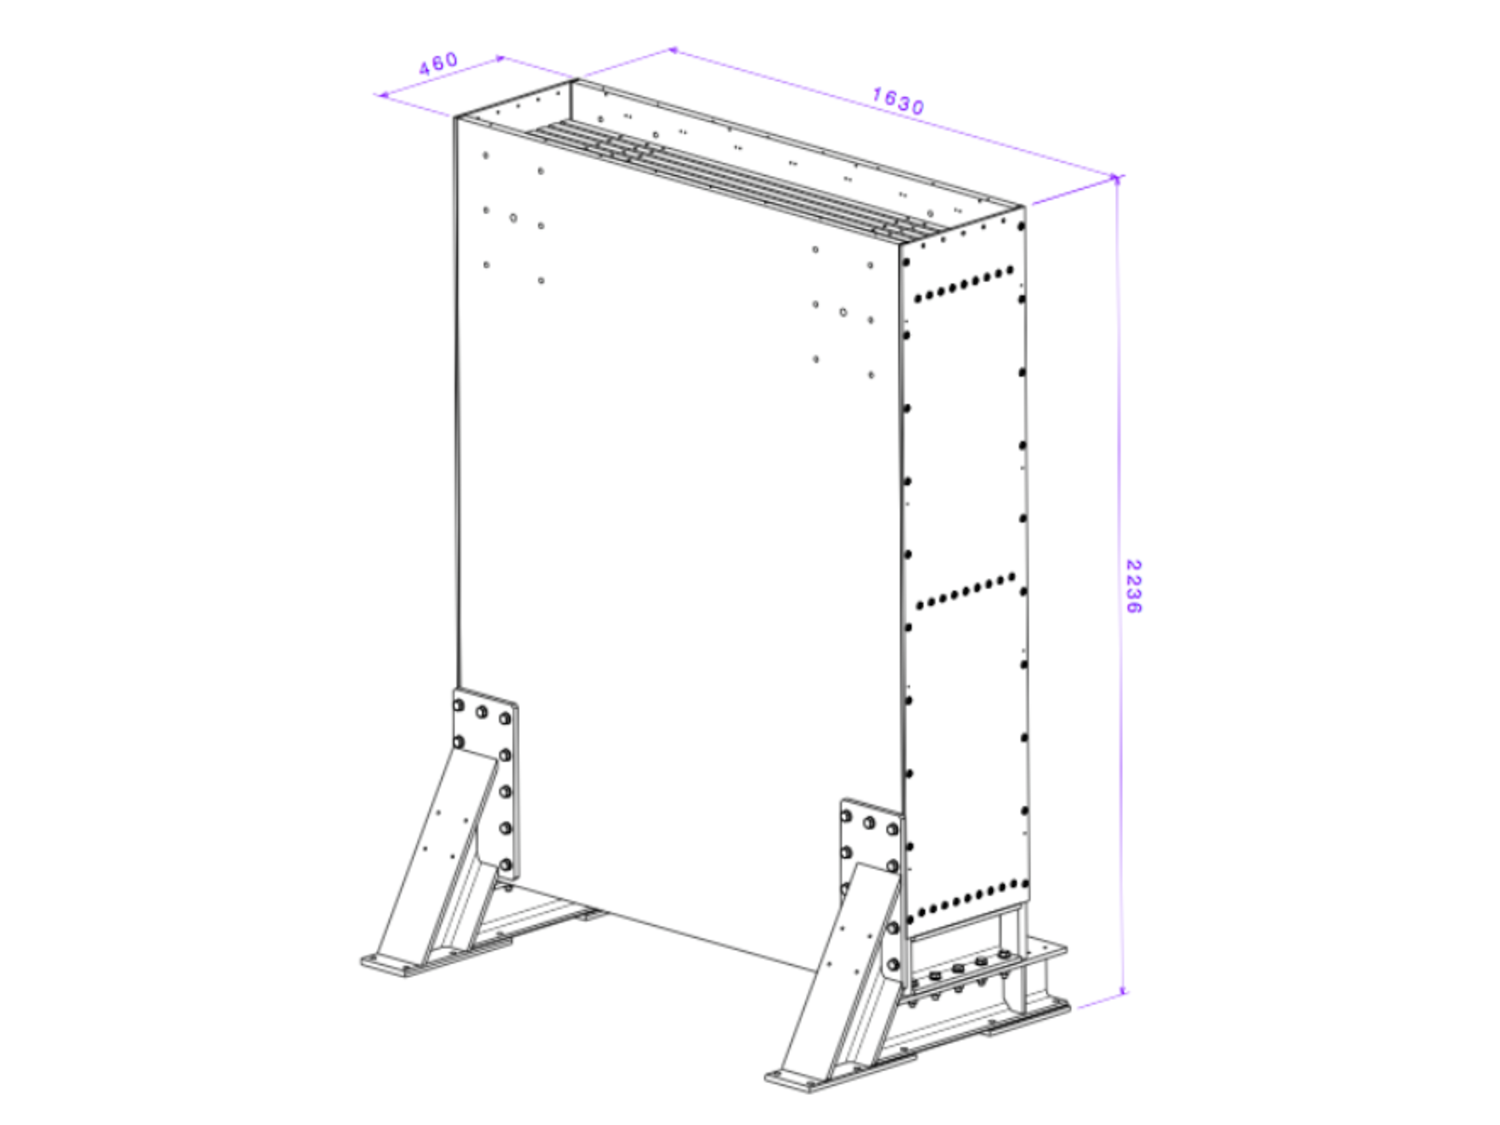
\includegraphics[width=0.8\linewidth]{fig/side_mrd_structure.pdf}
\end{center}
\caption{
Support structure of the Side-MRD module.
}
\label{fig:side_mrd_support_structure}
\end{figure}

\begin{figure}[tbh]
\begin{center}
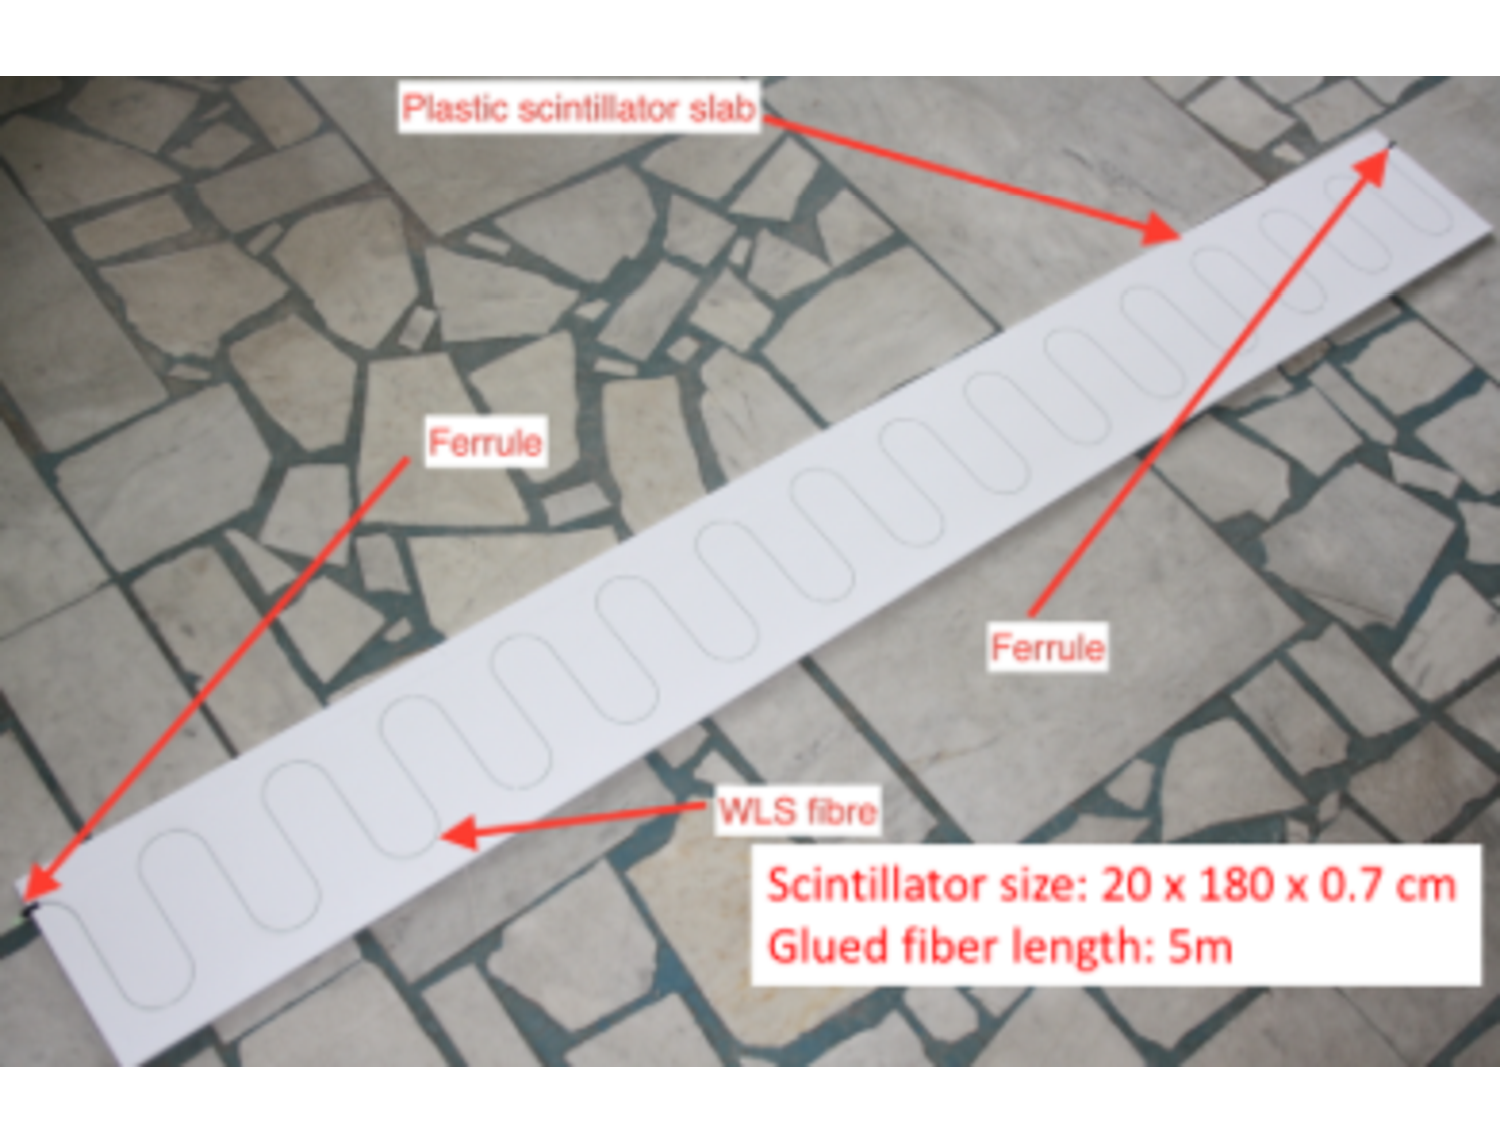
\includegraphics[width=0.8\linewidth]{fig/side_mrd_scintillator.pdf}
\end{center}
\caption{
Scintillator bar of the Side-MRD modules.
}
\label{fig:side_mrd_scintillator}
\end{figure}

\begin{figure}[tbh]
\begin{center}
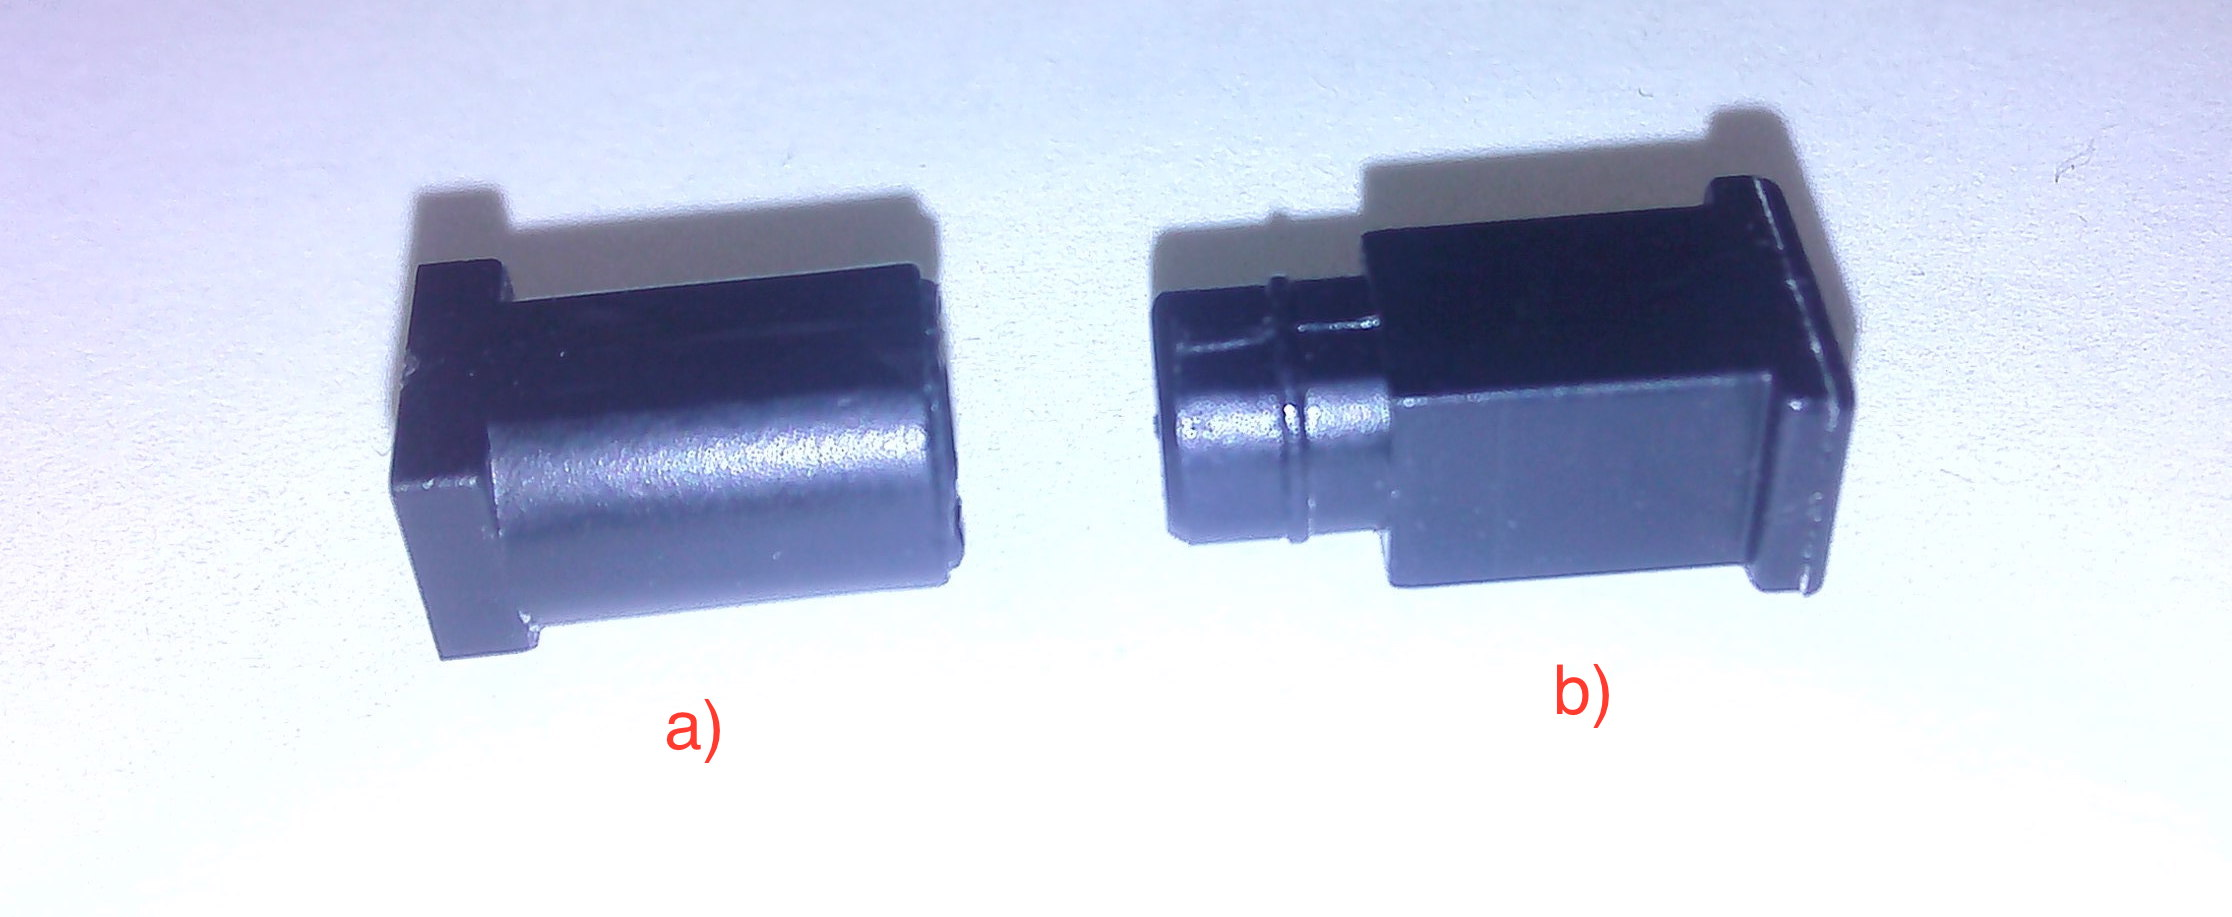
\includegraphics[width=0.8\linewidth]{fig/side_mrd_optical_con.jpg}
\end{center}
\caption{
Optical connector for the Side-MRD scintillator. a) MPPC cover. b) Ferrule.
}
\label{fig:side_mrd_optical_con}
\end{figure}

\begin{figure}[tbh]
\begin{center}
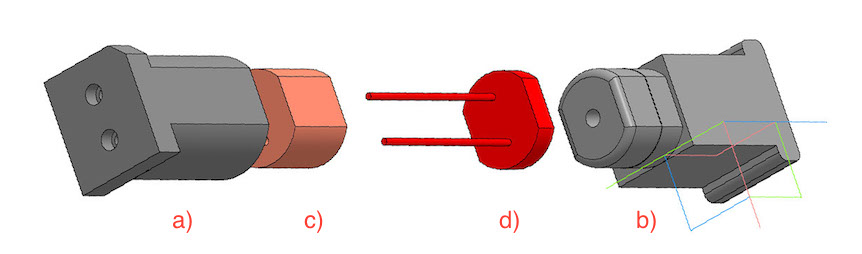
\includegraphics[width=0.8\linewidth]{fig/side_mrd_optical_scheme.jpg}
\end{center}
\caption{
Scheme of the MPPC placement in optical connector.  a) MPPC cover. b) Ferrule. c) Spring (sponge rubber). d) MPPC.
}
\label{fig:side_mrd_optical_scheme}
\end{figure}

Construction of scintillator bars of the Side-MRD modules had been completed in Russia, and they were transported to Japan in July 2017. 
Construction of Side-MRD modules will be done from November 2017 to January 2018 at Yokohama National University, then they will be transported to J-PARC and will be installed to the B2 floor of the T2K near detector hall before staring the T2K beam in March 2018.

\section{Physics goals}
We will measure the differential cross section for the charged current interaction on $\mathrm{H_2O}$ and/or CH.
The water-scntillator mass ratio of the Wagasci module is as high as 5:1 and the high purity measurement
of the cross section on $\mathrm{H_2O}$ is possible.
\textcolor{red}{One experimental option is to replace one of the two Wagasci module with the T2K proton module
  which is fully made with plastic scintillators. It will allow the precise comparison
  of cross section between $\mathrm{H_2O}$ and CH and also comparison of cross sections with ND280.}
  \textcolor{red}{Another option is to remove water from one of the two Wagasci module. 
The water-out WAGASCI module will make it possible to measure wider- angle scatterings for CH target and will provide a low density medium for the detection of low momentum protons.
The water-out WAGASCI data also can be used to subtract the background from interaction with scintillators in the water target measurement .
}
Our setup would allow the measuemrents of inclusive and also exclusive channles such as
1-$\mu$, 1-$\mu 1p$, 1-$\mu 1\pi{\pm} np$ samples, former two of which are mainly caused by the quasi-elastic and
2p2h interaction and the latter is mainly caused by resonant or coherent pion production and deep elastic scattering.
In general, an accelerator produced neutrino beam spectrum is wide and the energy reconstruction
somehow rely on the neutrino interaction model.
Therefore, recent neutrino cross section measurement results including T2K are given as a flux-integrated cross section
rather than cross sections as a function of the neutrino energy to avoid the model dependency.
We can provide the flux-averaged cross section.
In addition, by combining our measurements with those at ND280, model-independent extraction of the cross section
for narrow energy region becomes possible.
This method was demonstrated in \ref{ingrid_energy_dependent} and also proposed by P** (NUPRISM).
\textcolor{red}{add Yasutome plot here or later.}


\subsection{Expected number of events}
Expected number of neutrino events after the event selections is evaluated with Monte Carlo simulations as we will discuss in Section \ref{sec:mc_study}.
$2.41 \times 10^{4}$ CC events are expected in two WAGASCI modules after the selection with $1\times 10^{20}$ POT in neutrino-mode, and its purity is 75.5 \%.
In case we choose the option with one WAGASCI module and the T2K proton module,  $1.2 \times 10^{4}$ CC events are expected in the WAGASCI module and $\sim 1\times 10^{4}$ CC events are expected in the T2K proton module.
In case we choose the option with one water-in WAGASCI module and one water-out WAGASCI module,  $1.2 \times 10^{4}$ CC events are expected in the water-in module and $0.24 \times 10^{4}$ CC events are expected in the water-out module.


\subsection{Nuclear effects}
In T2K experiment, neutrinos interact with bound nucleons in relatively heavy nuclei (Carbon and Oxygen), so the cross-section is largely affected by nuclear effects.
The nuclear effects are categorized as nucleons' momentum distribution in nucleus, interactions with  correlated pairs of nucleons in nucleus (two particles-two holes, 2p2h), corrections from collective nuclear effects calculated with Random Phase Approximation (RPA) and final state interactions (FSI) of secondary particles in the nuclei after the initial neutrino interactions.





The 2p2h interactions mainly happen through $\Delta$ resonance interactions following a pion-less decay and interactions with a correlated nucleon pair.
The 2p2h interactions are observed in electron scattering experiments (add ref. here) where the 2p2h events observed in the gap between Quasi-Elastic region and Pion-production region as shown in Fig. \ref{fig:electrono_scattering_data}.
Neutrino experiments also attempt to measure the 2p2h interactions, but separation of the QE peak and the 2p2h peak is more difficult because transferred momentum (p) and energy (w) are largely affected by  neutrino energy which cannot be determined event-by-event in the wide energy spectrum of the accelerator neutrino beam.
Our model-independent narrow neutrino spectra extracted from combined analyses of our data and ND280 data are ideal for searching the 2p2h interaction because clearer separation of the QE peak and the 2p2h peak is expected.


The corrections from collective nuclear effects calculated by RPA as a function of $Q^{2}$ are shown in Fig. \ref{fig:effect_rpa}.
The $Q^{2}$ dependence of the correction can be tested by measuring angular distribution of muons in CC1-$\mu$ and CC1-$\mu 1p$ events.
The uncertainties of the corrections in low (high) $Q^{2}$ regions can be constrained by observing the events with a forward-going (high-angle) muon, so it is essential to measure muon tracks with full acceptance.


T2K experiment is starting to use $\nu_{e}$ CC1$\pi$ events for its CP violation search to increase the statistics.
One of the biggest uncertainty of CC1$\pi$ sample comes from the final state interactions of pions in the nuclei after the initial neutrino interactions because they change the multiplicity, charge and kinematics of the pions.
The multi-pion production events can be migrated into the CC1$\pi$ sample due to the FSIs, and they become important backgrounds.
We can constrain the uncertainties from the pion FSIs by measuring pion rescattering in the detector and pion multiplicity in CCn$\pi$ sample with low detection threshold and full acceptance for pion tracks.
The water-out WAGASCI can provide good sample for the pion FSI studies because its low density medium enables the detection of low momentum pions in addition to the full acceptance.


\section{Status of J-PARC T59 experiment}
We had submitted a proposal of a test experiment to J-PARC in April 2014 to test a new detector with a water target, WAGASCI, at the neutrino monitor hall, and the proposal was approved as J-PARC T59.
The project contains the side and downstream muon range detectors as well.

The first WAGASCI module has been constructed in 2016 and installed at the on-axis position in front of the T2K INGRID detector for the commissioning and the first cross section measurement as a part of the T2K experiment.
The INGRID electronics boards are used to read the signal.
The light yield measured with muons produced by the interaction of neutrinos
in the hall wall, shown in Fig.~\ref{fig:wmlight}, is sufficiently high to get good hit efficiency.  
%
\begin{figure}[tbh]
\begin{center}
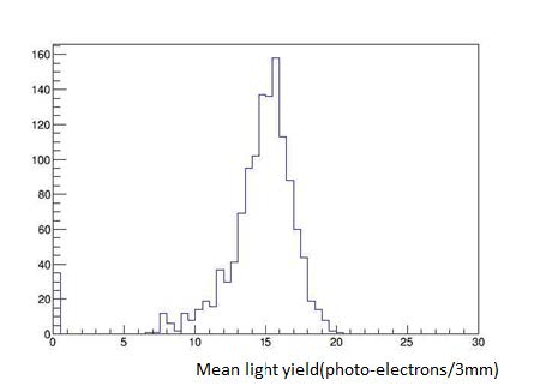
\includegraphics[width=0.5\linewidth]{fig/wmlight.pdf}
\end{center}
\caption{Light yield for muons produced by the interaction of neutrinos
  in the hall wall. Average light yields for each channel are plotted.
}
\label{fig:wmlight}
\end{figure}
A track search algorithm based on the cellular automaton has been developed using the software tools by the T2K INGRID. 
Examples of observed events are shown in Fig.~\ref{fig:onaxis_eventdisplay}
The tracking efficiency in 2-dimensional projected plane was evaluated by comparing the reconstructed track
in the WAGASCI module and the INGRID module and shown in Fig.\ref{fig:wmefficiency}.
Note that that the tracking efficiency for high angle ($>70\deg$) is not evaluated because of the acceptance
of the INGRID module, not because of the limitation of the WAGASCI module.
\begin{figure}[tbhp]
\begin{center}
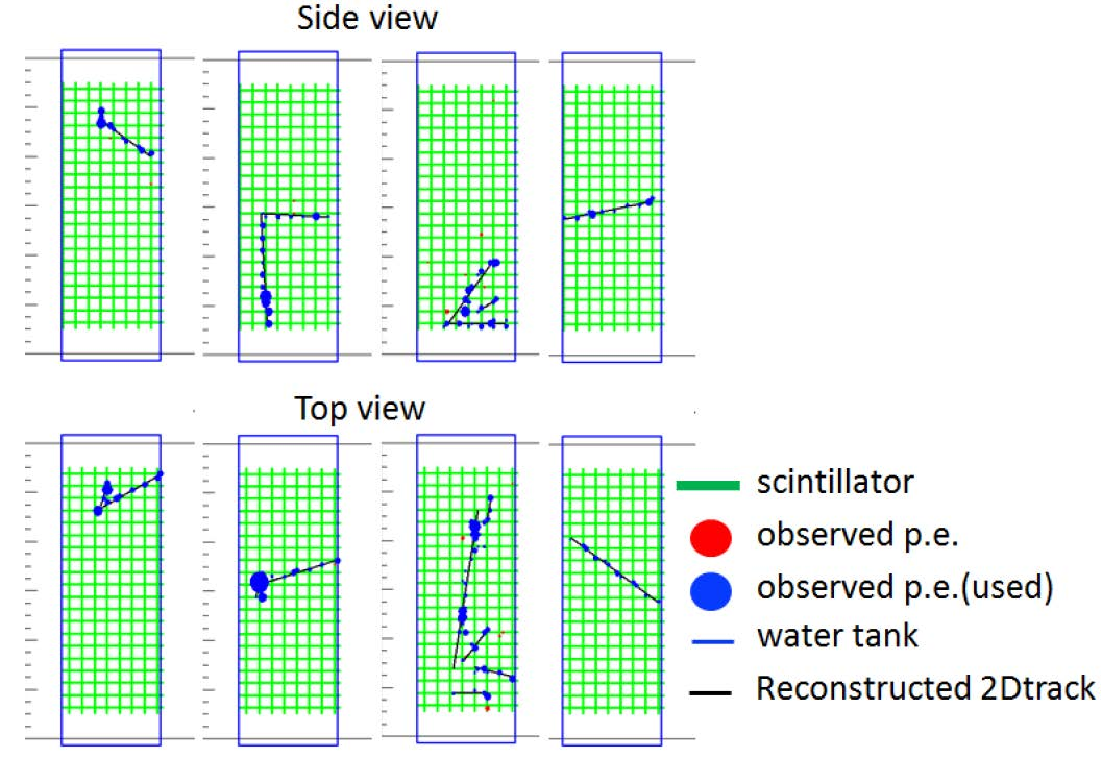
\includegraphics[width=\textwidth]{fig/wagascieventdisp.pdf}
%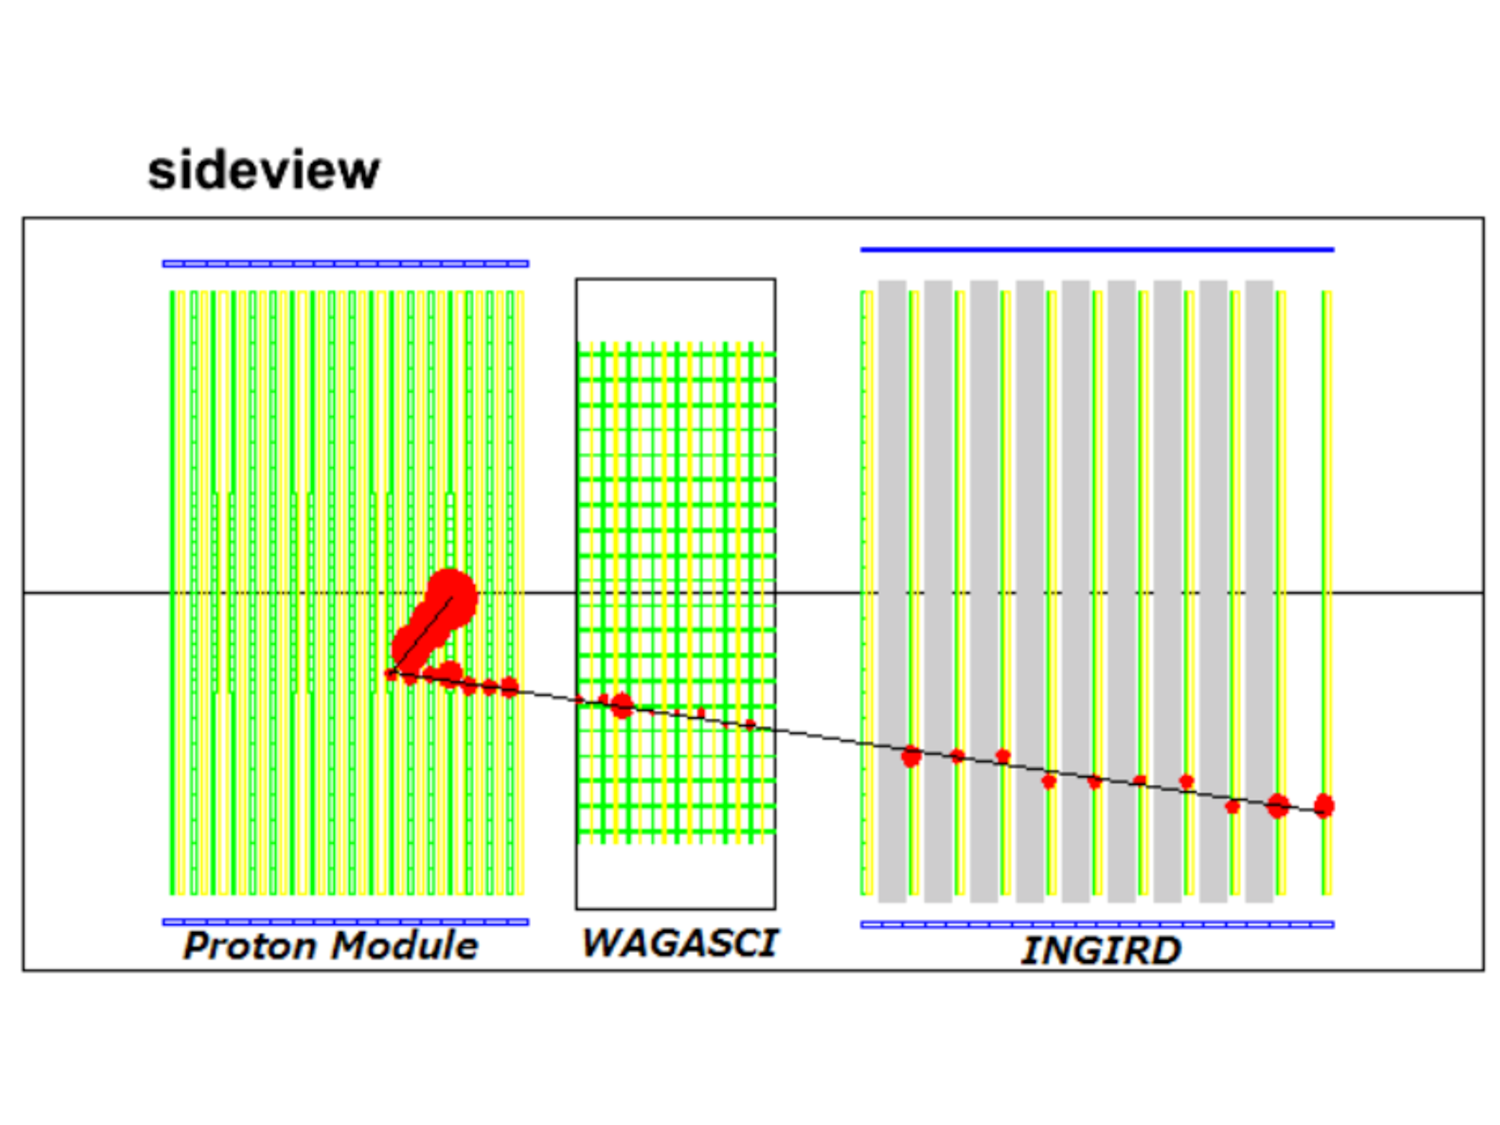
\includegraphics[width=0.8\linewidth]{fig/t59_event_display_oct_dec_2017.pdf}
% \includegraphics[width=0.8\linewidth]{fig/all_detector2.pdf}
\end{center}
\caption{
  Example event displays of the WAGASCI module at on-axis.
  The reconstructed tracks are overlaid.}
\label{fig:onaxis_eventdisplay}
%  t59_event_display_oct_dec_2017}
\end{figure}
%
\begin{figure}[tbhp]
  \begin{center}
   \begin{subfigure}{0.48\textwidth}
     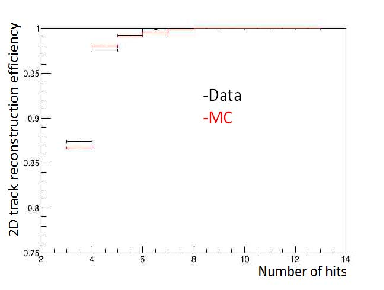
\includegraphics[width=\linewidth]{fig/wmeffvshit.pdf}
    \end{subfigure}
  \begin{subfigure}{0.48\textwidth}
      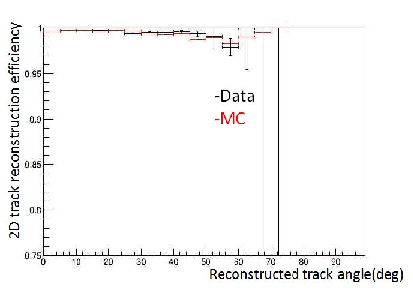
\includegraphics[width=\linewidth]{fig/wmeffvsangle.pdf}
    \end{subfigure}    
    \end{center}
  \caption{2D track reconstruction efficiency as a function of number of hits (left) and track angle (right).
  Here the track angle is the one reconstructed by the INGRID module.}
\label{fig:wmefficiency}
\end{figure}

In 2017 Autumn, the construction of the second WAGASCI module and the dedicated electronics board were completed.
The module and the electronics were install to the B2 floor together with the T2K proton module and the INGRID
module as shown in Fig.~\ref{fig:det_confg_oct_dec2017}.
The proton module is to be used as the entering muon veto and also for the comparison of interaction between CH and Water.
The INGRID module is for the temporary muon detector with limited acceptance for this period.
The detector was commissioned and is in operation to take data with the antineutrino beam during the T2K beam time from October.

 \begin{figure}[tbhp]
 \begin{center}
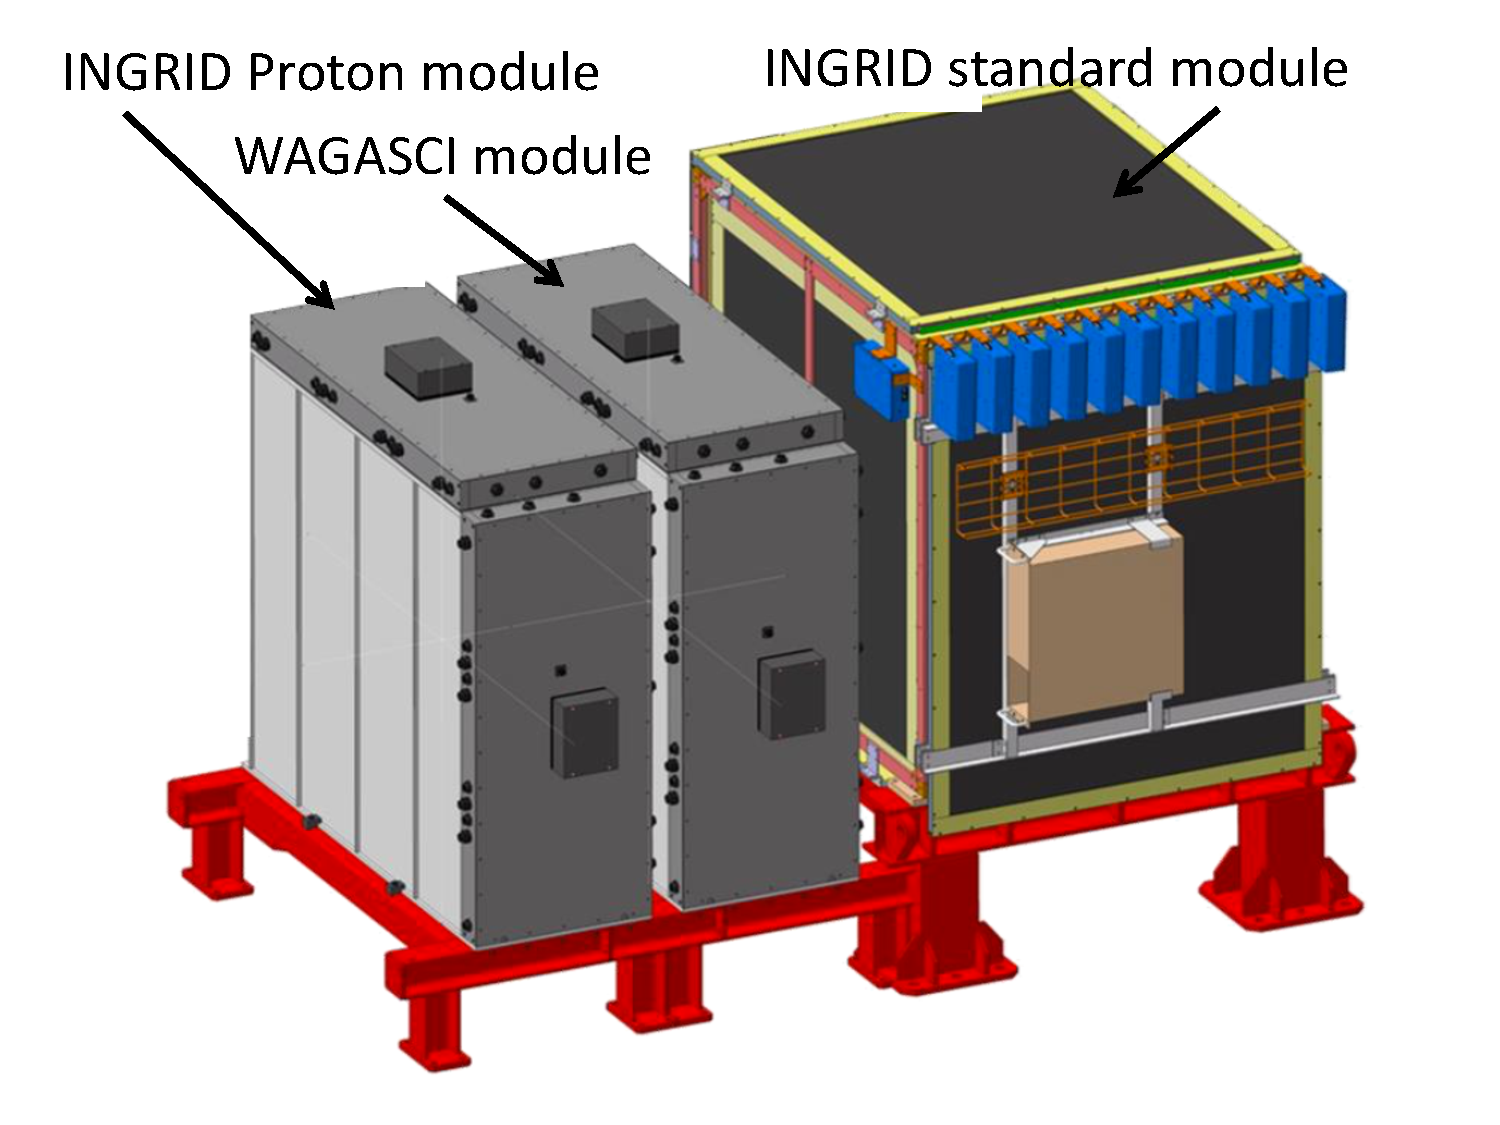
\includegraphics[width=0.5\linewidth]{fig/t59_det_config_oct_dec_2017.pdf}
 \end{center}
 \caption{
 J-PARC T59 detector configuration in October 2017.
 }
 \label{fig:det_confg_oct_dec2017}
 \end{figure}

The production of the components of the side muon range detectors has been completed and now the detectors
are being assembled at the Yokohama National University.
These detectors will be installed sometime from January to June, 2018 when T2K is not running.

The Baby MIND detector was transported from CERN to Japan in December, 2017.
It will be installed and commissioned in Jan.-Feb. 2018 and T59 will take the neutrino-induced muon data in April and May.

%Fist, the start time of neutrino beam measurement is changed from December 2015 to October 2017, and the requested neutrino beam is changed from $1\times10^{21}$ POT of $\nu$ beam to $0.8\times10^{21} $POT of anti-$\nu$ beam. 
% Second, the detector configuration is changed. In the original proposal, central neutrino detector are expected to be surrounded by newly developed muon-range detectors (MRDs), but we will use spare neutrino detectors of the T2K experiment instead of them during neutrino beam measurement from October to December 2017. Construction of the newly developed MRDs, Baby-MIND and Side-MRD, is in progress, and they will be installed to the both sides and the downstream of the central neutrino detector from January to March 2018. Then, we will resume neutrino beam measurements from March 2018 and will take the neutrino beam data until May 2018.


%\subsection{On-axis beam measurement with Prototype detector}
%Add INGRID water module measurement here.

%\subsection{Plans from October 2017 to May 2018}
%J-PARC MR will extract its proton beam to T2K neutrino beam-line from October to December 2017, and, from March to May 2018. 
%T2K experiment will produce anti-neutrino beam and will accumulate $\sim8\times10^{20}$ POT data during the above period.


% J-PARC T59 will perform neutrino beam measurements on the B2 floor of the T2K near neutrino detector hall during the above period to test basic performances of the WAGASCI detector and new electronics. During the beam measurements from October to December 2017, one WAGASCI module will be placed between spare neutrino detectors of the T2K experiment, INGRID Proton module and INGRID standard module. 
 % as shown in Fig. \ref{fig:det_config_oct_dec2017}.
% Detector location on the B2 floor of T2K near detector hall is shown in Fig. \ref{fig:det_loc_oct_dec2017}. 
%Here, the INGRID Proton module is used as a charged particle VETO detector and, the INGRID standard module is used as a downstream muon detector. 
%We had submitted a proposal to use these spare neutrino detectors for the T59 neutrino beam measurements to the T2K collaboration, and we got an approval from T2K. 


 
% \begin{figure}[tbh]
% \begin{center}
% 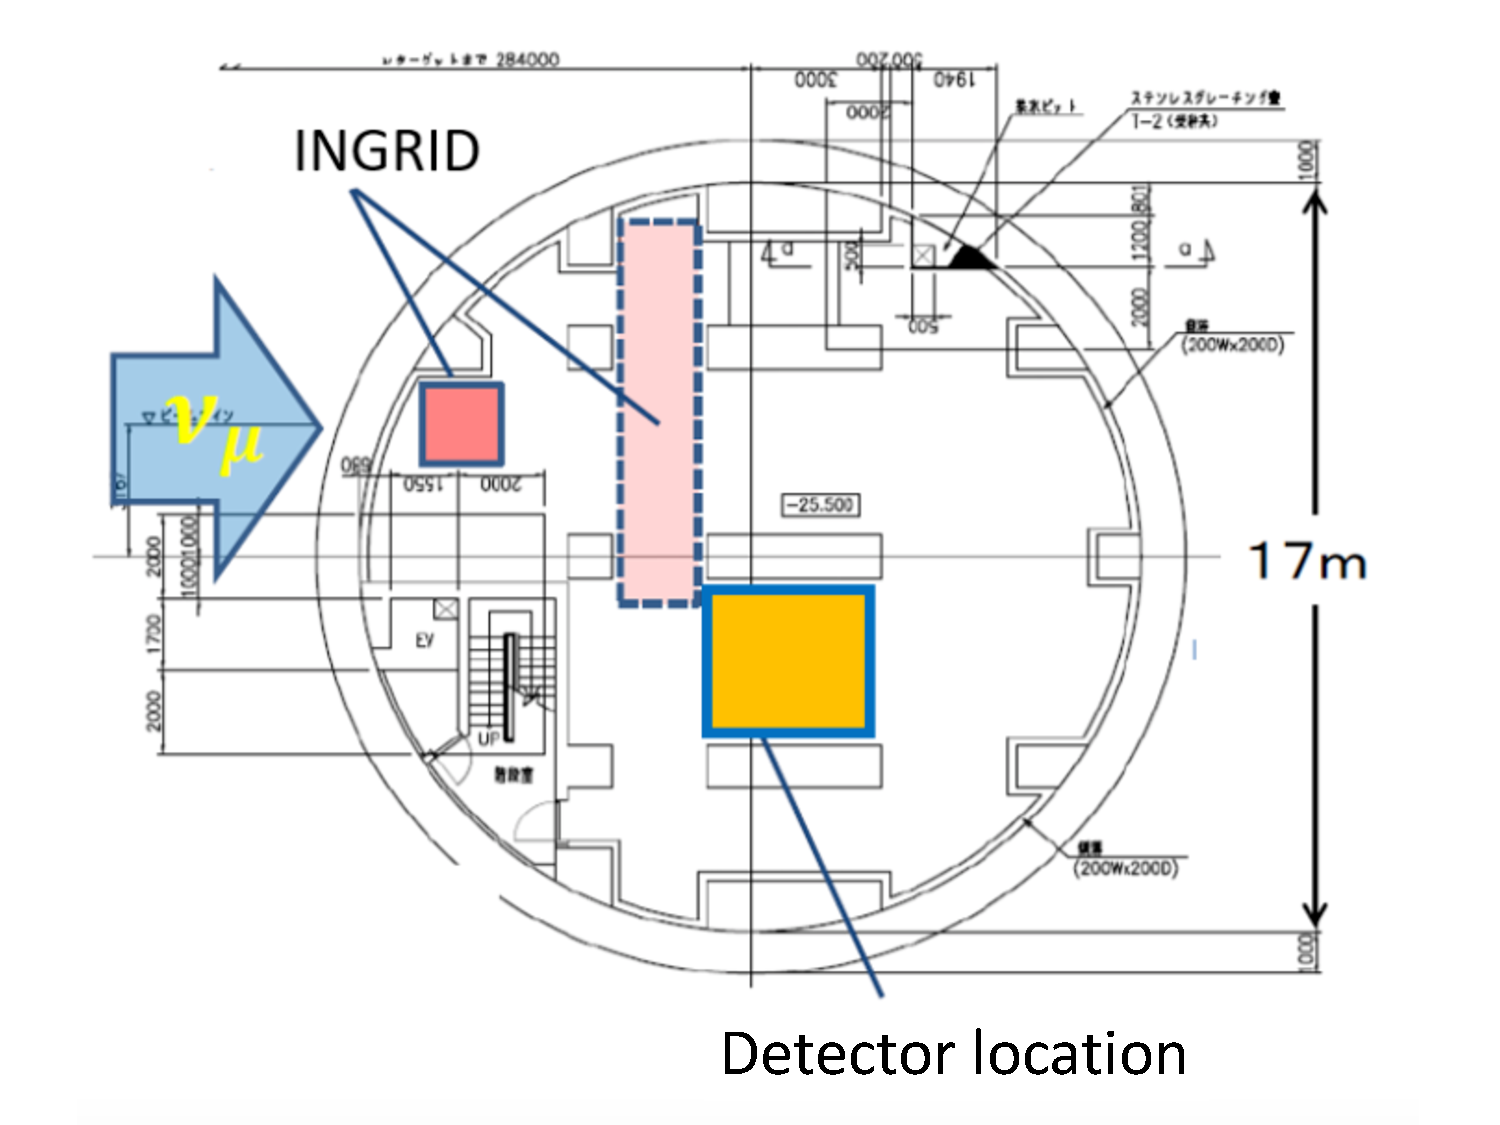
\includegraphics[width=0.8\linewidth]{fig/t59_det_location_oct_dec_2017.pdf}
% \end{center}
% \caption{
% J-PARC T59 detector location from Oct. to Dec. 2017
% }
% \label{fig:det_loc_oct_dec2017}
% \end{figure}


%During the beam measurements from March to May 2018, Baby-MIND and two side muon-range detector (Side-MRD) modules will be installed on the downstream and the both sides of the WAGASCI detector, as shown in Fig. \ref{fig:det_config_mar_may2018}, to increase angular acceptance for secondary charged particles from neutrino interactions.
 
%\begin{figure}[tbh]
%\begin{center}
%
\includegraphics[width=0.8\linewidth]{fig/tmp.pdf}
% \includegraphics[width=0.8\linewidth]{fig/all_detector2.pdf}
%\end{center}
%\caption{
%J-PARC T59 detector configuration with Baby-MIND and two Side-MRD modules from Mar. to May 2018.
%(Need to prepare the figure.)}
%\label{fig:det_config_mar_may2018}
%\end{figure}


%Expected number of neutrino events in the WAGASCI detector during the above beam period is evaluated with Monte Carlo simulations. 
%Neutrino beam flux at the detector location is simulated by T2K neutrino flux generator, JNUBEAM, neutrino interactions with target materials are simulated by a neutrino interaction simulator, NEUT, detector responses are simulated using GEANT4-based simulation. 
%The neutrino flux at the detector location, 1.5 degrees away from the J-PARC neutrino beam axis, is shown in Figure \ref{fig:b2flux}, and its mean neutrino energy is around 0.68 GeV.


%To perform the detector performance test, the following event selections are applied to the data. 
%First, track reconstructions are performed in the WAGASCI detector, and the reconstructed vertex is required to be inside a defined fiducial volume, $80 \times80 \times 32$ cm$^{3}$ region at the center of the detector, to reduce contamination from external backgrounds. 
%Second, at least one charged particle is required to reach to INGRID standard module or Side-MRD modules, and it makes more than two hits in these sub-detectors. 
%With the event selection, expected numbers of the neutrino-candidate events during the beam period are summarized in Table 1. 
%Using the data, we will test the detector performance with $\sim3$\% statistical uncertainties.









%\section{Detector performance}
%\subsection{Wagasci module}

\begin{figure}[tbh]
\begin{center}
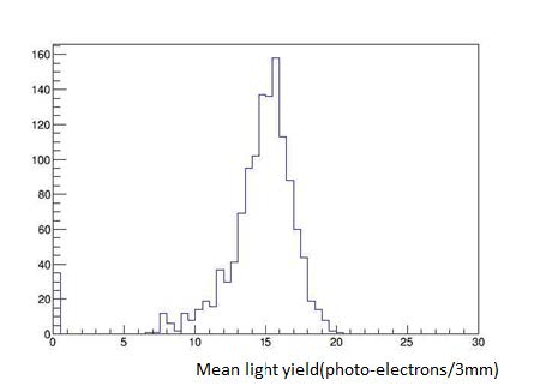
\includegraphics[width=0.5\linewidth]{fig/wmlight.pdf}
\end{center}
\caption{Average light yield for muons produced by the interaction of neutrinos
  in the hall wall.
}
\label{fig:wmlight}
\end{figure}

\begin{figure}[tbh]
  \begin{center}
    \begin{subfigure}{0.48\textwidth}
      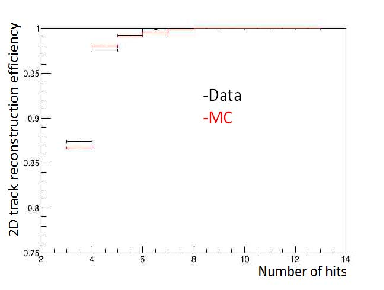
\includegraphics[\linewidth]{fig/wmeffvshit.pdf}
    \end{subfigure}
    \begin{subfigure}{0.48\textwidth}
      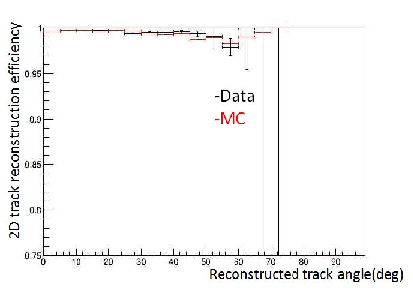
\includegraphics[\linewidth]{fig/wmeffvsangle.pdf}
    \end{subfigure}    
    \end{center}
  \caption{2D track reconstruction efficiency as a function of number of hits (left) and track angle (right).}
\label{fig:wmefficiency}
\end{figure}

%\subsection{Baby MIND}
The Baby MIND construction was completed in June 2017, and it was then tested in June and July 2017 at the Proton Synchrotron experimental hall at CERN with a mixed particle beam comprising mostly muons whose momenta could be selected between 0.5 and 5 GeV/c. An event display from the summer 2017 tests is shown in Figure \ref{beam_vs_cosmic}.

\inserttwographs{0.45}{baby_mind_Wagasci_rough_cad.png}{0.50}{baby_mind_layout.png}{Left) WAGASCI modules: flanked by 2 side muon range detectors (sMRD) and one downstream muon detector (Baby MIND). Right) side view layout of the Baby MIND during beam tests at CERN.}{wagasci-layout}


\insertgraph{1.0}{comparing_beam_cosmics.png}{Comparison of a beam muon and cosmic muon in the three different geometrical projections of the detector. The beam impinges on the detector from the left. The arrows indicate the direction of travel of these muons. The direction of the cosmic muon is inferred from timing information.}{beam_vs_cosmic}


All counters were measured at INR Moscow with a cosmic ray setup using the same type S12571-025C MPPCs and CAEN DT5742 digitizer \cite{Antonova:2017cdw}. The average light yield (sum from both ends) was measured to be 37.5 photo-electrons (p.e.) per minimum ionizing particle (MIP) and 65 p.e./MIP for vertical and horizontal counters, respectively. After shipment to CERN, all counters were tested once more individually with an LED test setup \cite{led_test_system}. 0.1\% of counters failed the LED tests and were therefore not used during the assembly of modules. 

%\subsection{Side muon range detector}

\section{MC studies}
\label{sec:mc_study}
\subsection{Simulation setup}
\label{sec:mc_setup}
The expected number of neutrino events in the water-in Wagasci detector
is predicted by Monte Carlo simulations.
Neutrino beam flux at the detector location is simulated by T2K neutrino flux generator, JNUBEAM. Neutrino interactions with target materials are simulated by a neutrino interaction simulator, NEUT. Detector responses are simulated using GEANT4-based simulation.


The detector geometry in the simulation so far is different from the actual setup as shown in Figure \ref{fig:wagasci_mc_geometry}.
The active neutrino target region consists of four WAGASCI modules.
The size of the WAGASCI module is same as the actual one: 1000 mm $\times$ 1000 mm in the x and y directions and 500 mm along the beam direction (z-direction).
%An event display of a MC event in the WAGASCI detectors is shown in Figure \ref{fig:wagasci_event_display}.
Two Side-MRD modules are installed either side of the Wagasci modules.
Each Side-MRD module consists of ten iron plates whose dimension is 30 mm (thickness) $\times$ 2000 mm (height) $\times$ 3200 mm (width). 
The distance between the Side-MRD modules and WAGASCI modules is 800 mm.
The downstream-MRD is equivalent to the Baby-MIND, but without the magnetic field.
It consists of thirty iron plates whose dimension is  30 mm (thickness) $\times$ 2000 mm (height) $\times$ 4000 mm (width).
The distance between the downstream-MRD modules and WAGASCI modules is 800 mm.
Update of the study with the actual geometry is now underway.

\begin{figure}[tbhp]
\begin{center}
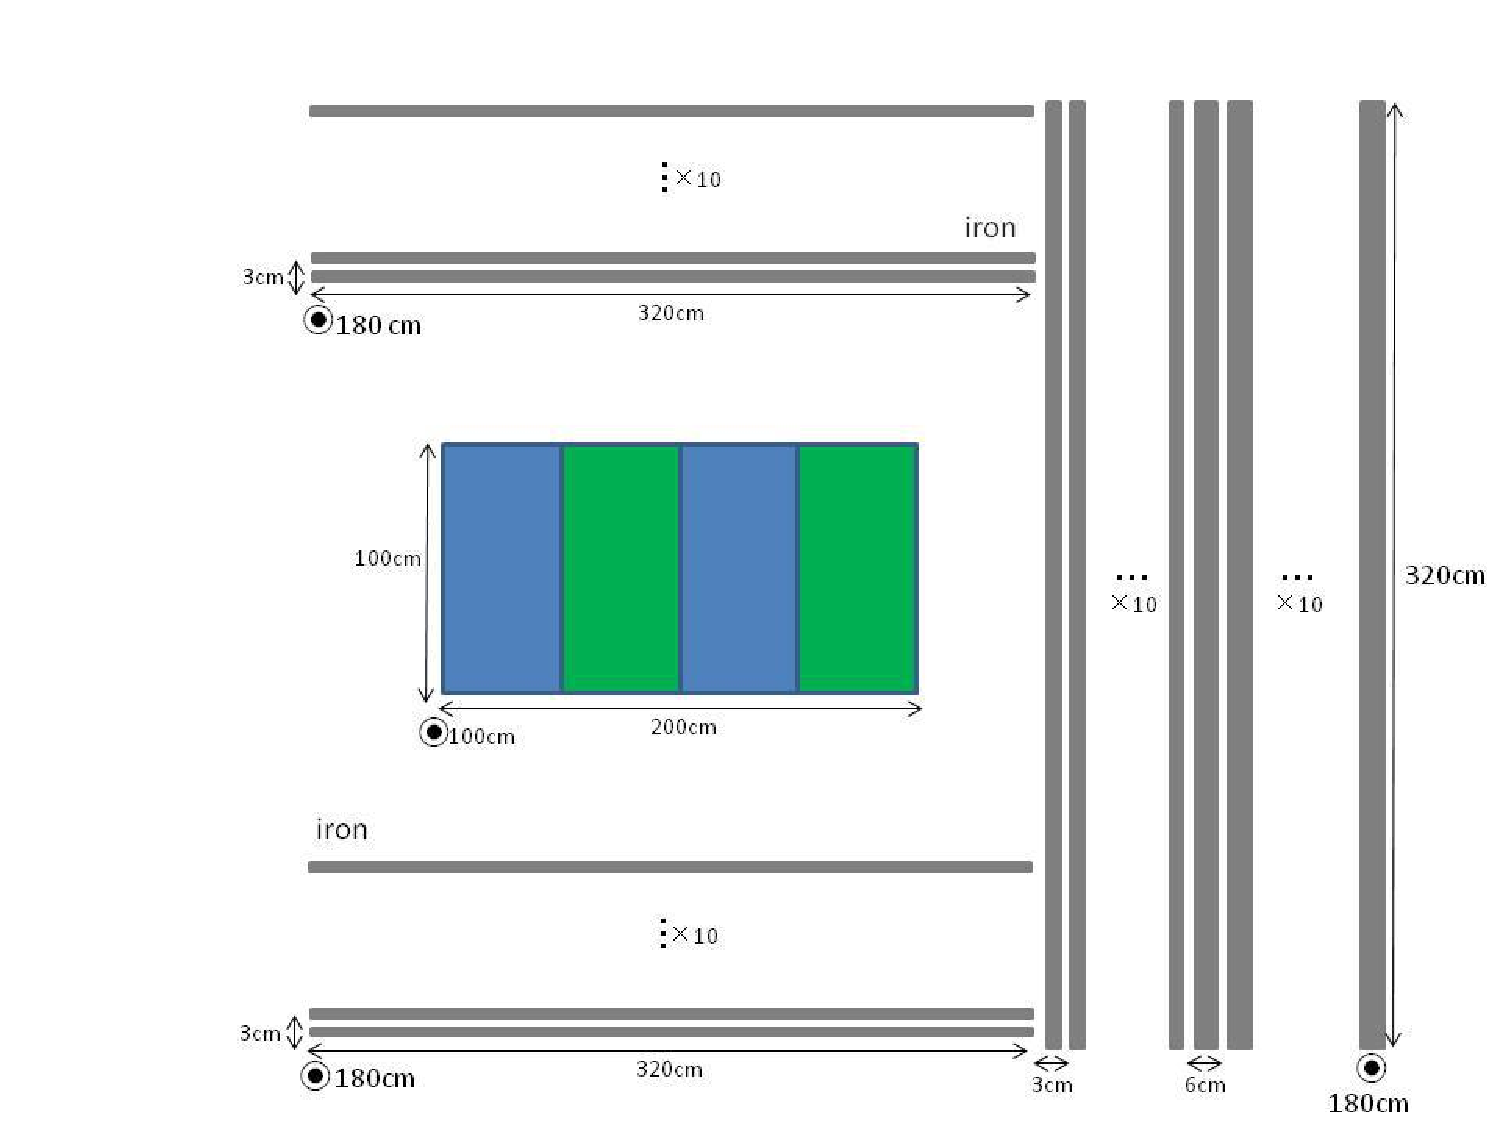
\includegraphics[width=0.8\linewidth]{fig/wagasci_mc_geometry.pdf}
% \includegraphics[width=0.8\linewidth]{fig/all_detector2.pdf}
\end{center}
\caption{
Geometry of the detectors in the Monte Carlo simulation.}
\label{fig:wagasci_mc_geometry}
\end{figure}

%\begin{figure}[tbh]
%\begin{center}
%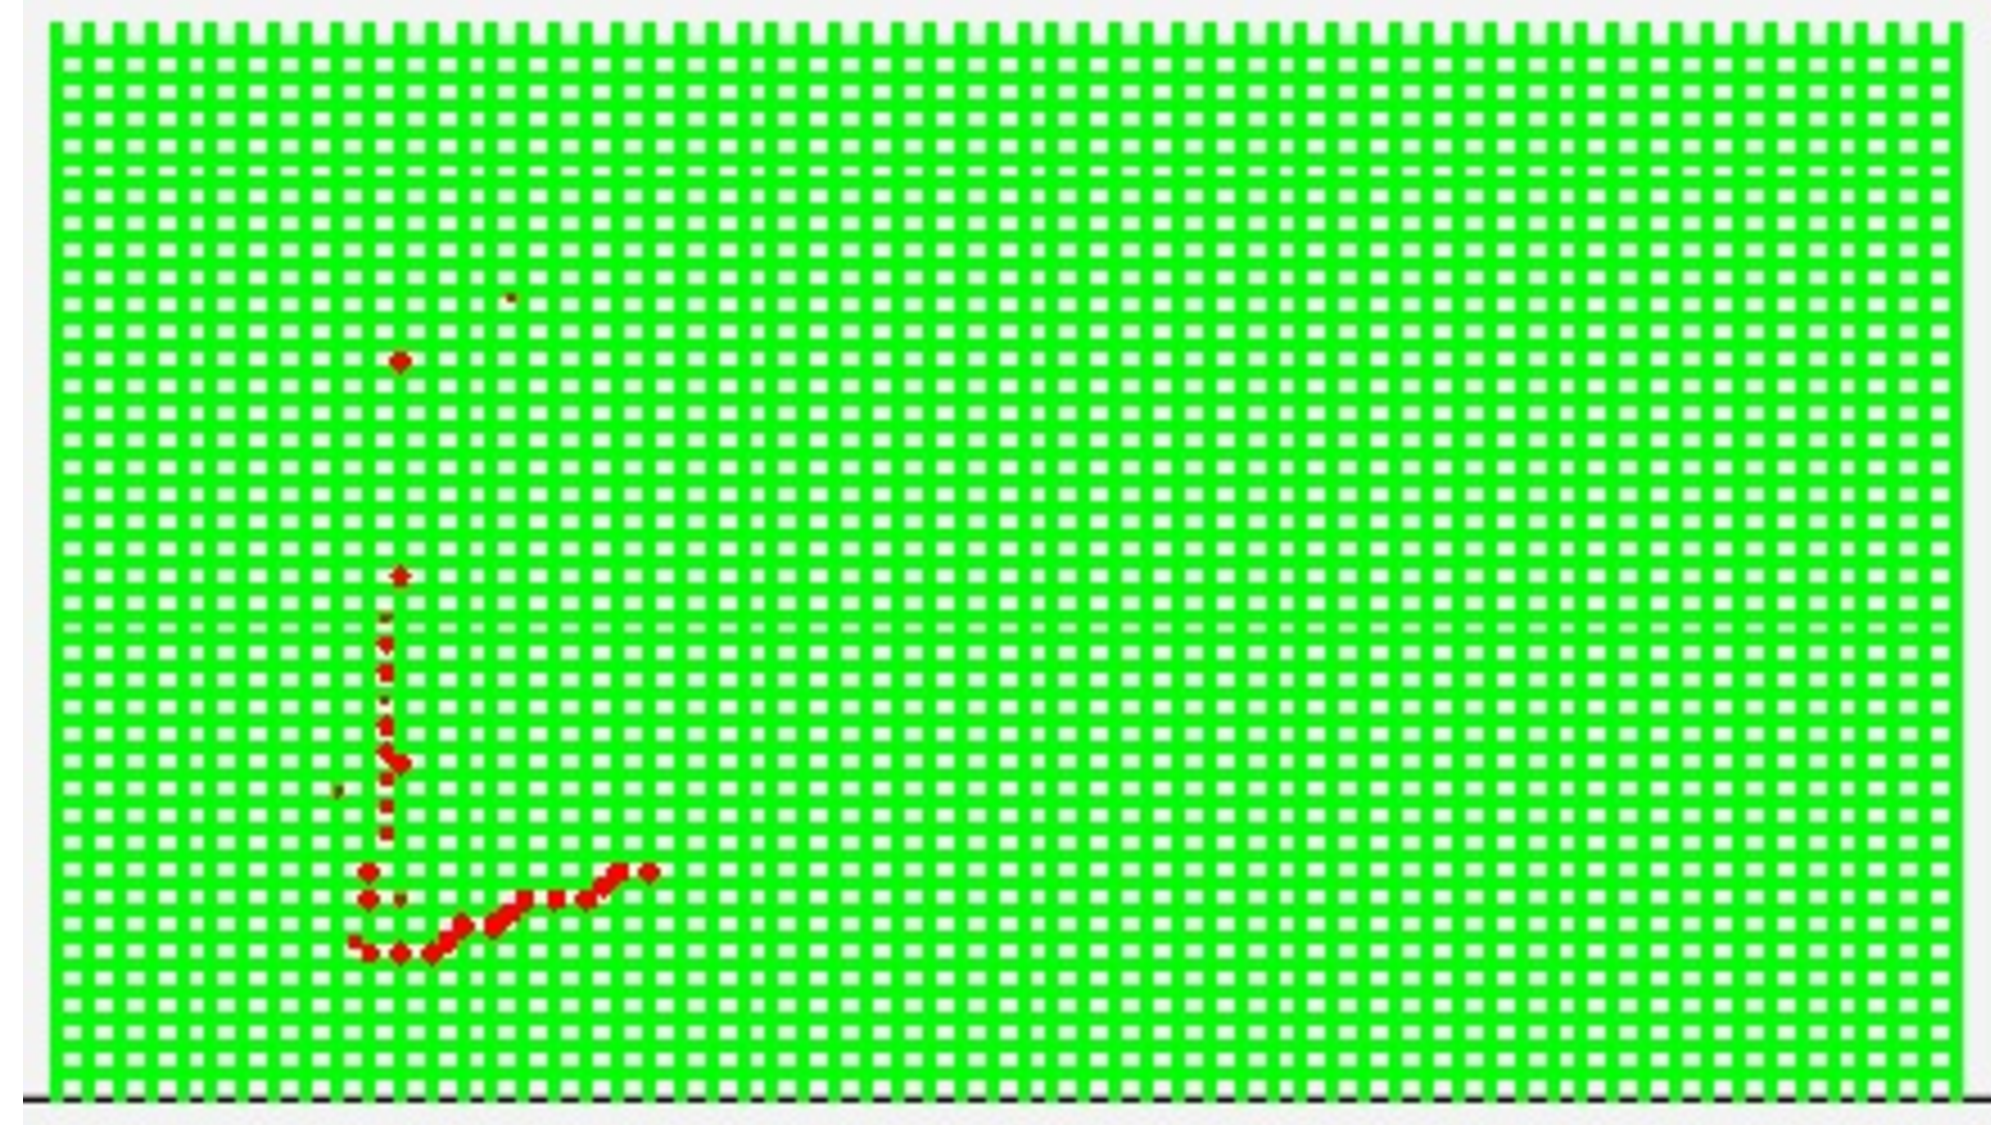
\includegraphics[width=0.8\linewidth]{fig/wagasci_event_display.pdf}
%% \includegraphics[width=0.8\linewidth]{fig/all_detector2.pdf}
%\end{center}
%\caption{
%An event display of MC event in WAGASCI detectors. Green lines are scintillators and red circles are the hit channels.}
%\label{fig:wagasci_mc_geometry}
%\end{figure}

% In order to estimate backgrounds from neutrino interactions in the wall and floor of the experimental hall, the geometry of the experimental hall is implemented in the GEANT4-based detector simulation.

To simulate the signal, the energy deposit inside the scintillator is converted into the number of photons. 
The effects of collection and attenuation of the light in the scintillator and the WLS fiber are simulated, and the MPPC response is also taken into account. 
The light yield is smeared according to statistical fluctuations and electrical noise.


\subsection{Charged-current event selection}

Tracks are reconstructed in two-dimensional planes in each sub-detector.
Then, track matching among the sub-detectors and three-dimensional track reconstruction are performed.
These analysis tools have been developed from the software tools by the T2K INGRID and in mature stage already.

The events are selected as follows.
The starting point of the track is required to be 50~mm away from the edge of the WAGASCI module. This is to remove the background from the outside.
% as shown in Fig. \ref{fig:fv_cut}.
% \begin{figure}[tbh]
% \begin{center}
%   \begin{subfigure}{0.48\textwidth}
%     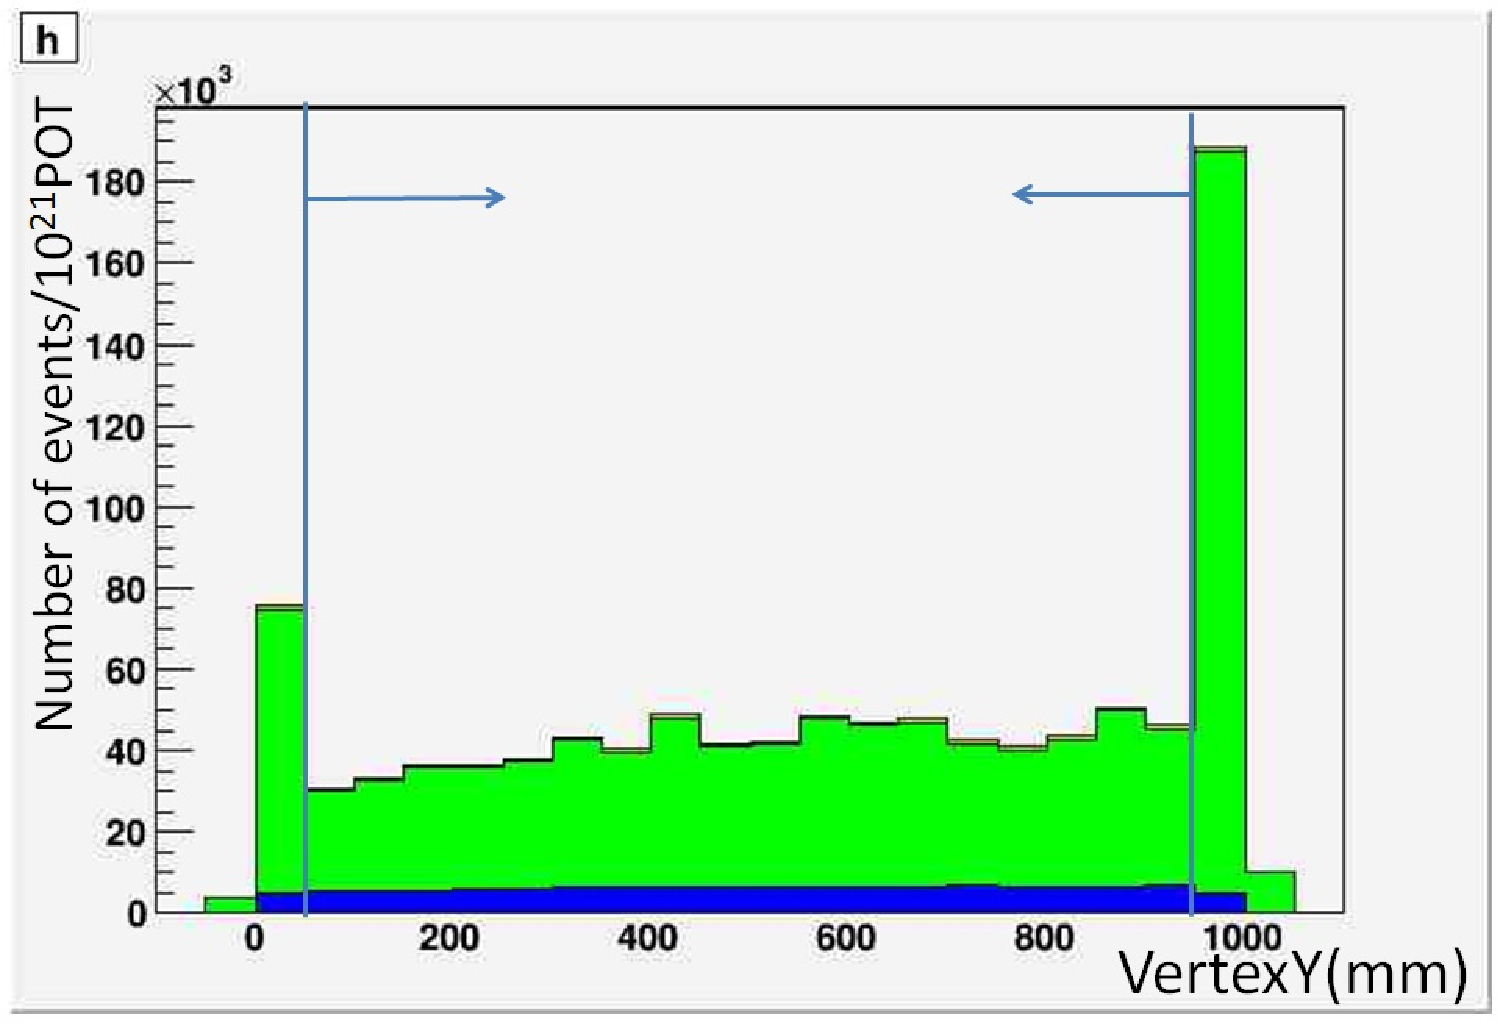
\includegraphics[width=\linewidth]{fig/fv_cut_y.pdf}
%    \end{subfigure}
%  \begin{subfigure}{0.48\textwidth}
%      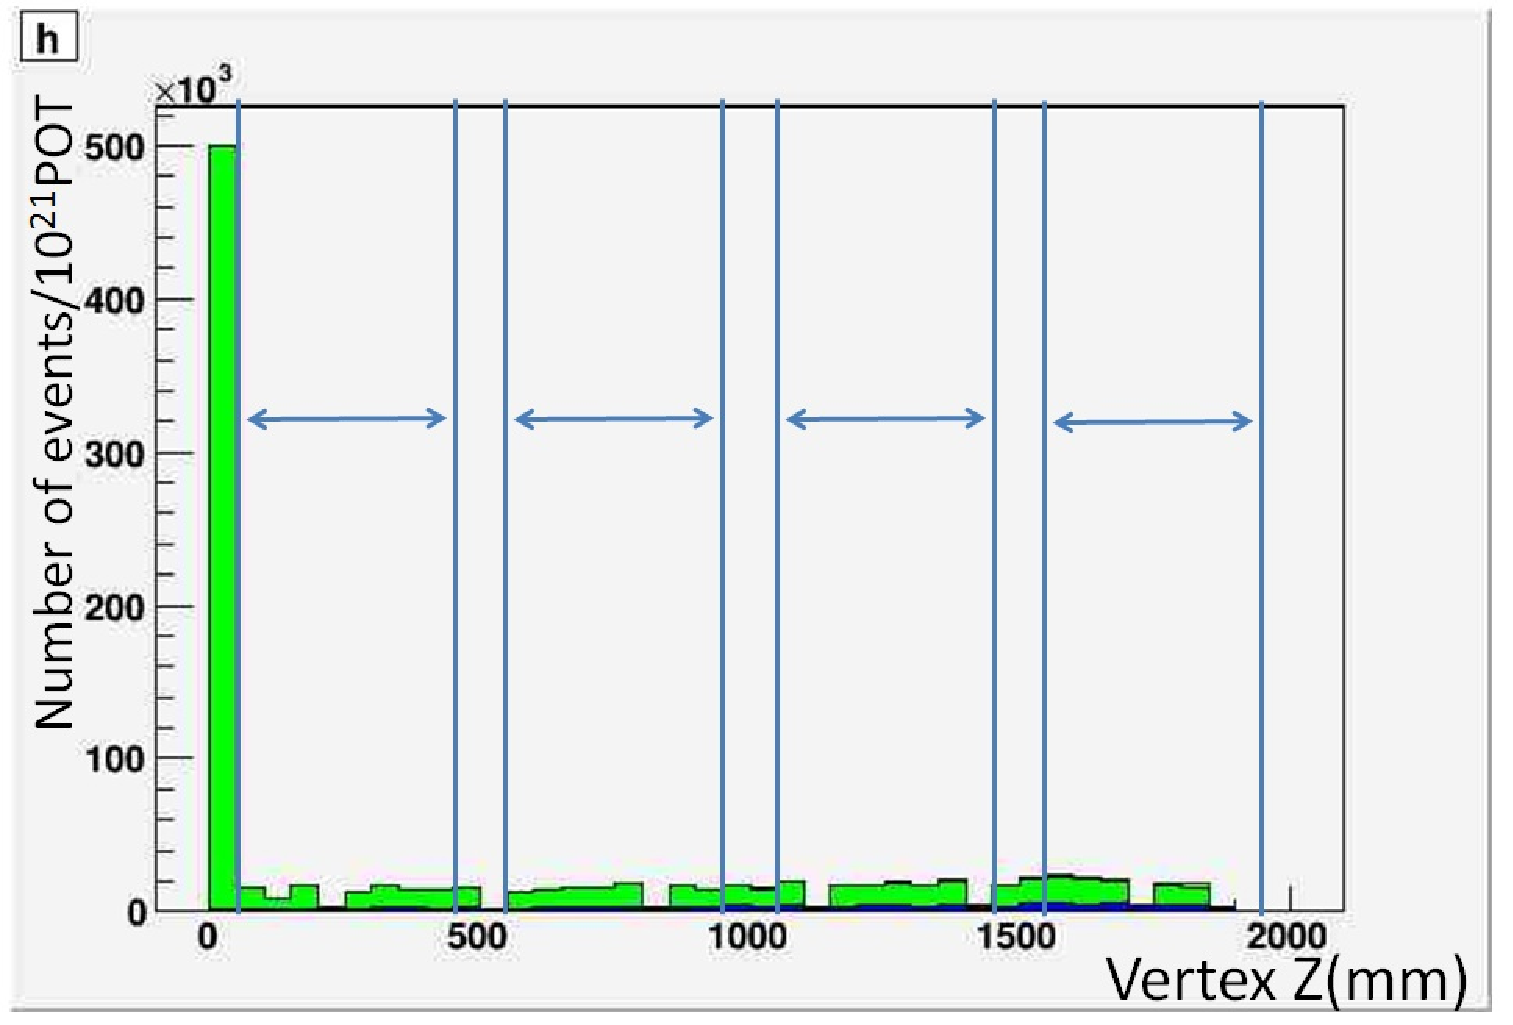
\includegraphics[width=\linewidth]{fig/fv_cut_z.pdf}
%    \end{subfigure}    
%    \end{center}
%  \caption{Event selection with the vertex of the track.
% Blue hist. are events from the WAGASCI modules, green hist. are events from the experimental hall, % and yellow hist. are events from the Side-MRD modules and the downstream-MRD.
% }
% \label{fig:fv_cut}
% \end{figure}
The longest track has to penetrate more than one (five) iron plates in Side-MRD modules (Baby-MIND).
This cut select a muon track and rejects backgrounds from NC and neutral particles.
%as shown in Figure \ref{fig:penetrated_iron_plates_cut}.
Then, in order to determine the muon momentum, it is required that the longest track stops in MRDs (Side-MRD modules and Baby-MIND) or penetrate all iron plates.
% \begin{figure}[tbh]
%  \begin{center}
%   \begin{subfigure}{0.48\textwidth}
%      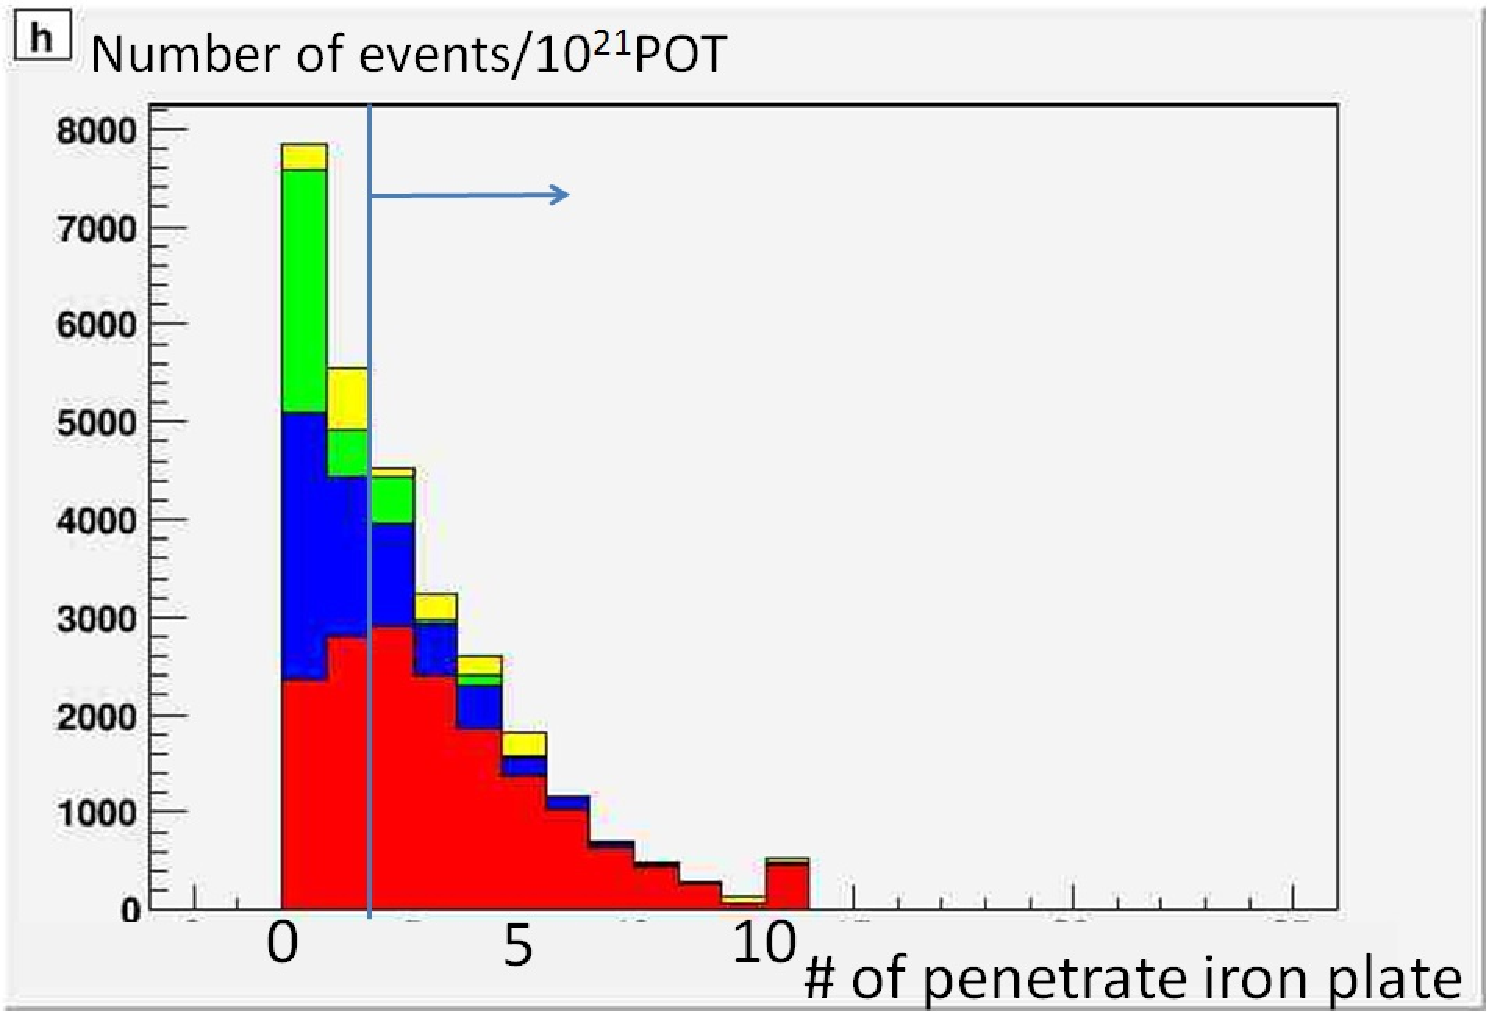
\includegraphics[width=\linewidth]{fig/penetrated_iron_plates_cut_sidemrd.pdf}
%     \end{subfigure}
%   \begin{subfigure}{0.48\textwidth}
%     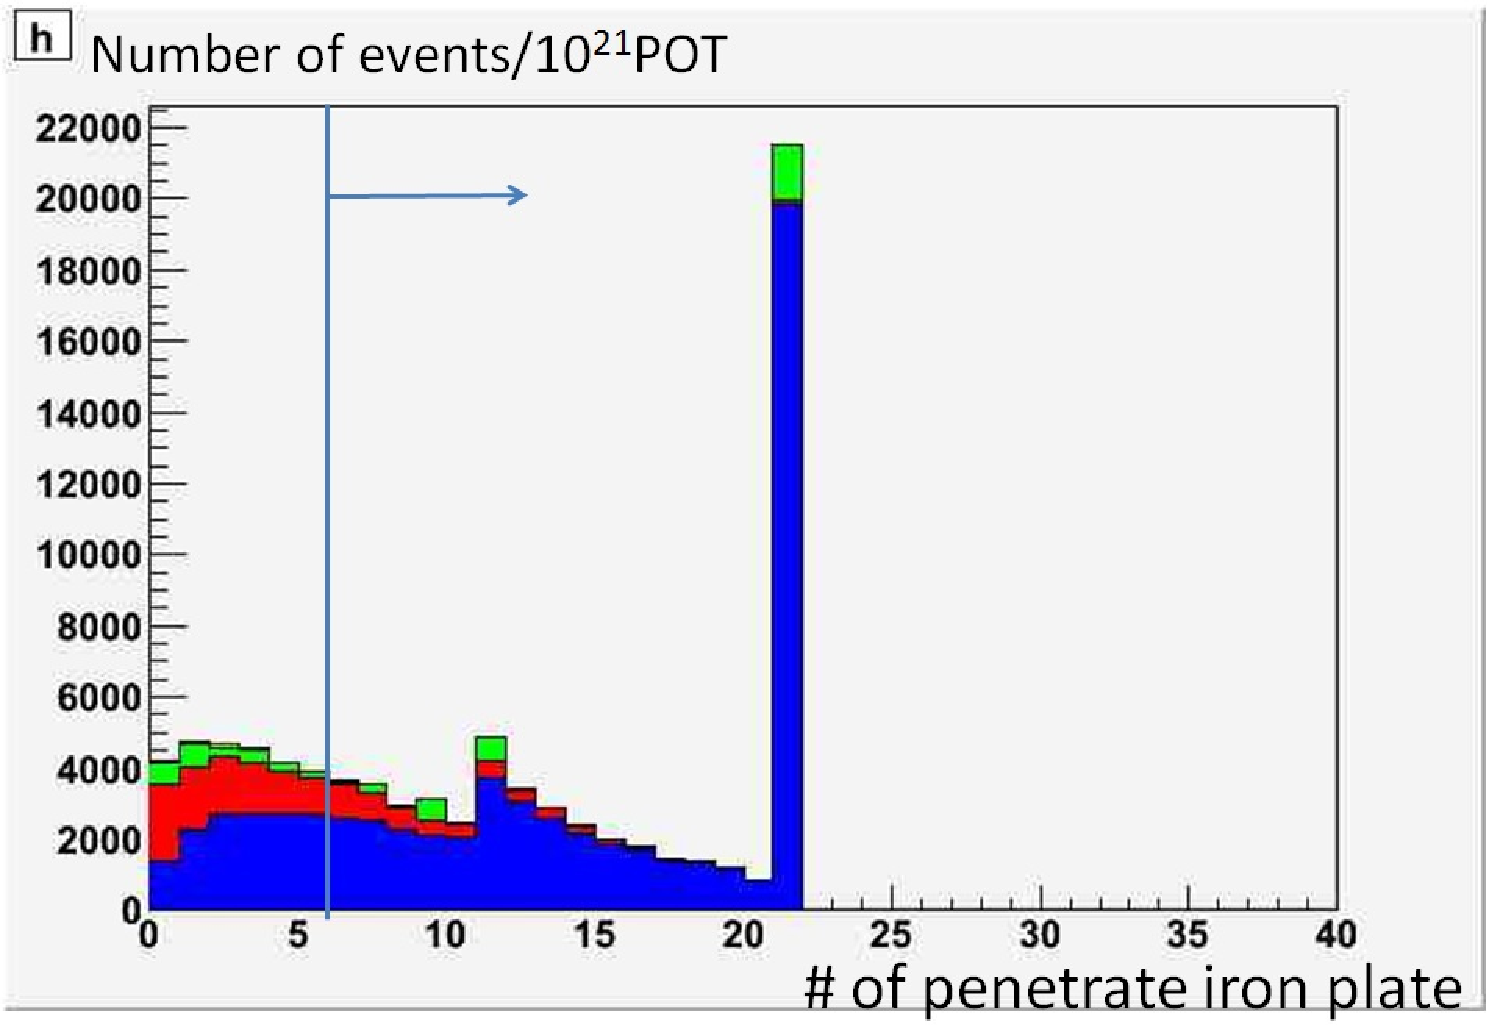
\includegraphics[width=\linewidth]{fig/penetrated_iron_plates_cut_babymind.pdf}
%     \end{subfigure}    
%     \end{center}
%   \caption{
% Event selection with the number of the penetrated iron plates in the side-MRD modules (left) and the Baby-MIIND (right).
% Blue and red hist. are events from the WAGASCI modules, green hist. are events from the experimental hall, and yellow hist. are events from the Side-MRD modules and the Baby-MIND.
% }
% \label{fig:penetrated_iron_plates_cut}
% \end{figure}

% \subsection{Selected events}


Table~\ref{tab:expected_num_events}  shows numbers of the selected events in one water-in WAGASCI module after the event selection.
We expect 4,239 (1,666) events from charged-current interaction on $\mathrm{H_2O}$ with $5 \times 10^{20}$  POT in (anti)neutrino-mode with one water-in WAGASCI module.
The purity, when interactions on CH is counted as background, is 78\% for the neutrino-mode.
There is a significant contamination from the wrong-sign (neutrino) interaction for antineutrino-mode, however, we expect that
it will be removed with efficiency higher than 90\% by Baby MIND.
%\begin{table}[htb]
%  \begin{center}
%    \caption{Expected number of the neutrino-candidate events in one water-in WAGASCI module with 1$\times 10^{21}$ POT in neutrino-mode.}
%    \begin{tabular}{c|ccc|c} \hline
%Cut   & CC & NC & Scinti Bkg. & Total \\ \hline
%Reconstructed & 18093.2 & 699.7 & 4698.3 & 23491.2 \\
%FV & 15150.8 & 588.4 & 3934.8 & 19673.9 \\
%Pene. iron & 11264.3 & 237.3 & 2875.4 & 14377.0 \\
%Stop/Penetrate MRDs & 8478.2 & 214.0 & 2173.1 & 10865.2 \\ \hline
%after all cuts & 78.0 \% & 2.0 \% & 20.0 \% & 100 \% \\
%\hline
%    \end{tabular}
%    \label{tab:expected_num_events_neutrino_beam}
%  \end{center}
%\end{table}
%\begin{table}[htb]
%  \begin{center}
%    \caption{Expected number of the antineutrino-candidate events in one water-in WAGASCI module with 1$\times 10^{21}$ POT in antineutrino-mode.}
%    \begin{tabular}{c|cccc|c} \hline
% Cut   & CC & NC & Scinti Bkg. & Wrong sign bkg & Total \\ \hline
%Reconstructed & 6499.7 & 107.3 & 2234.4 & 2330.8 & 11172.1 \\ 
%FV & 5457.9 & 89.3 & 1873.5 & 1946.6 & 9367.1 \\ 
%Pene. iron & 4172.3 & 30.8 & 1440.9 & 1560.6 & 7204.6 \\ 
%Stop/Penetrate MRDs & 3331.5 & 28.5 & 1120.3 & 1121.2 & 5601.5 \\ \hline
%after all cuts & 59.5 \% & 0.5 \% & 20.0 \% &  20.0 \% & 100 \% \\
%\hline
%    \end{tabular}
%    \label{tab:expected_num_events_antineutrino_beam}
%  \end{center}
%\end{table}
\begin{table}[htbp]
  \begin{center}
    \caption{Expected number of the selected neutrino-candidate events in one water-in WAGASCI module with $5\times 10^{20}$ POT in each of neutrino-mode and antineutrino-mode.
      Note that the wrong sign component will be reduced by one order by applying the charge selection by Baby MIND.}
    \begin{tabular}{ccccc} \hline
   & CC on $\mathrm{H_2O}$ & NC on $\mathrm{H_2O}$ & Interaction on CH  & wrong sign interaction\\ \hline
   $\nu$-mode & 4239 & 107 & 1087 & (negligible) \\ \hline
   anti-$\nu$-mode & 1666 & 14 & 560 & (561) \\
\hline
    \end{tabular}
    \label{tab:expected_num_events}
  \end{center}
\end{table}


Table \ref{tab:expected_num_cc_events} and \ref{tab:expected_num_ccfsi_events} summarize
contributions classified by the interaction types and final state topologies for the selected charged current-interaction events, respectively.
%
\begin{table}[htbp]
  \begin{center}
    \caption{Interaction types for the selected charged-current events.}
    \begin{tabular}{c|cccc} \hline
& CCQE & 2p2h & CC resonant $\pi$  & CC-DIS \\ \hline
$\nu$-mode & 48.4 \% & 9.7 \% & 27.1 \% & 14.7 \% \\
anti-$\nu$-mode &  57.1 \% & 8.2 \% & 17.3 \% & 17.3 \% \\
\hline
    \end{tabular}
    \label{tab:expected_num_cc_events}
  \end{center}
\end{table}
%
\begin{table}[htbp]
  \begin{center}
    \caption{Final state topologies for the selected charged-current events.}
    \begin{tabular}{c|cccc} \hline
& CC0$\pi$ & CC1$\pi$ & CC2$\pi$ & CCn$\pi$ \\ \hline
      $\nu$-mode & 67.4 \% & 20.9 \% & 3.0 \% & 8.7 \% \\ \hline
      anti-$\nu$-mode & 79.5 \% & 16.3 \% & 1.2 \% & 3.0 \% \\\hline
    \end{tabular}
    \label{tab:expected_num_ccfsi_events}
  \end{center}
\end{table}

Figure \ref{fig:angle_allcut} shows the reconstructed angles of the longest tracks in the selected events in the neutrino-mode and the anti-neutrino mode.
Figure \ref{fig:endpoint_longest_track} shows the iron plane numbers in Side-MRD and Baby-MIND corresponding to the end points of the longest tracks in the selected events in the neutrino-mode and the anti-neutrino mode.
%
\begin{figure}[tbh]
 \begin{center}
  \begin{subfigure}{0.48\textwidth}
     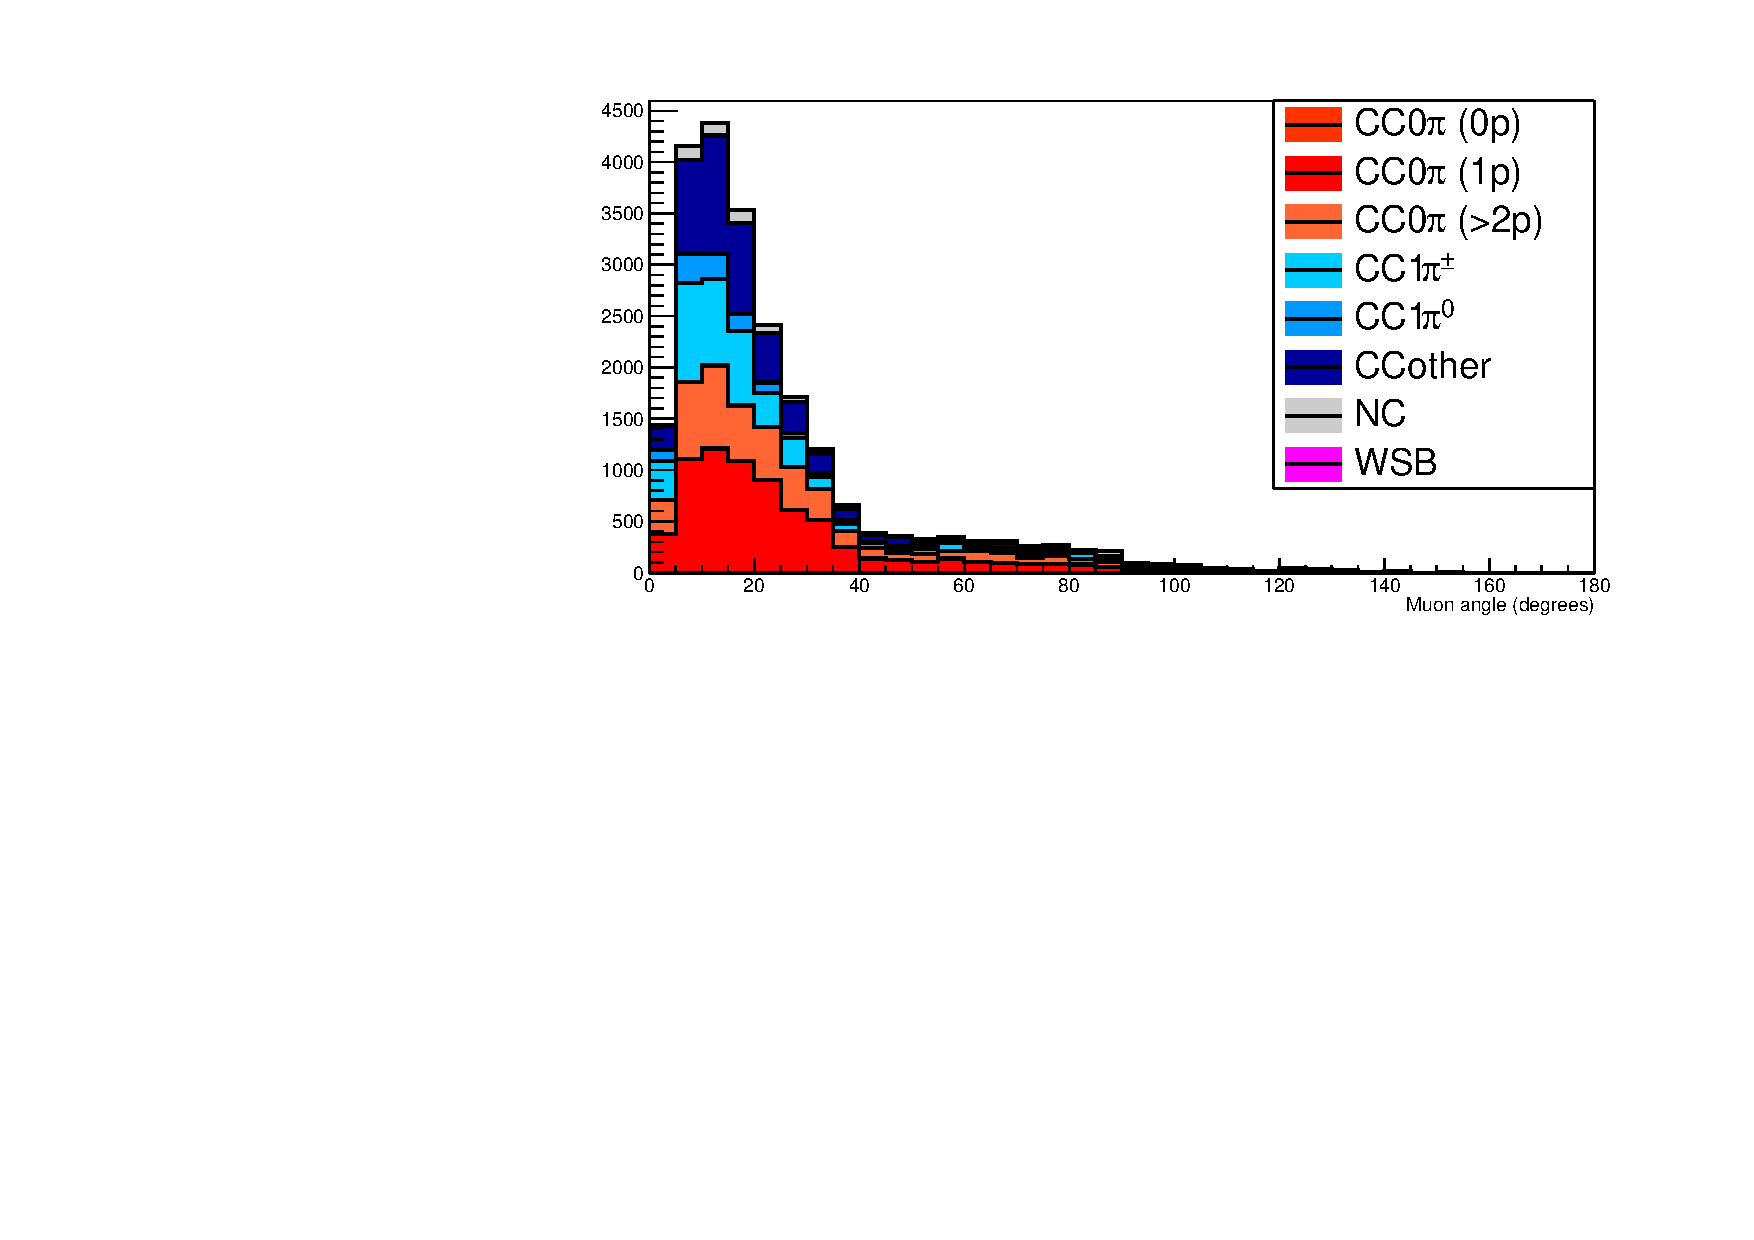
\includegraphics[width=0.55\linewidth, angle=270]{fig/FHCMuonAngle_StoppedOrThroughGoing.pdf}
%     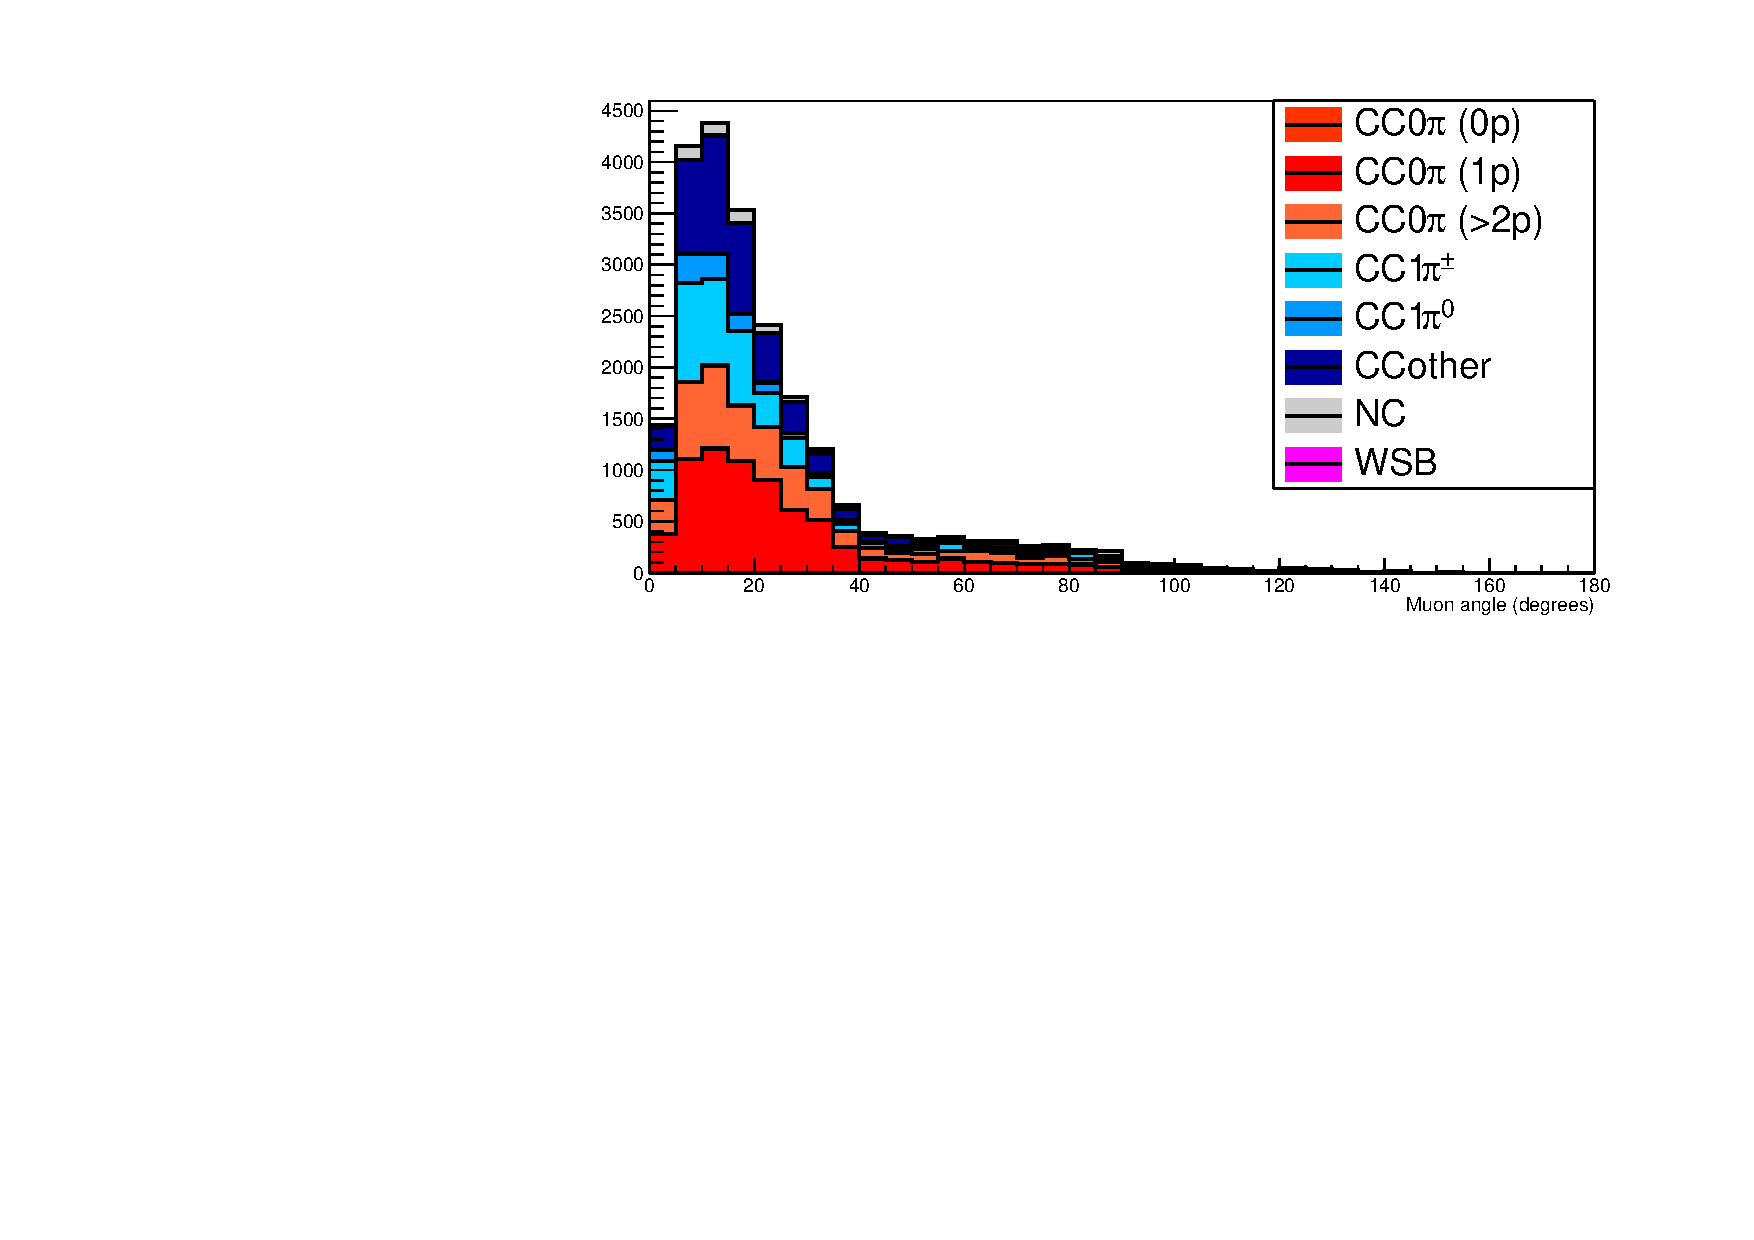
\includegraphics[width=\textwidth]{fig/FHCMuonAngle_StoppedOrThroughGoing.pdf}
    \end{subfigure}
  \begin{subfigure}{0.48\textwidth}
    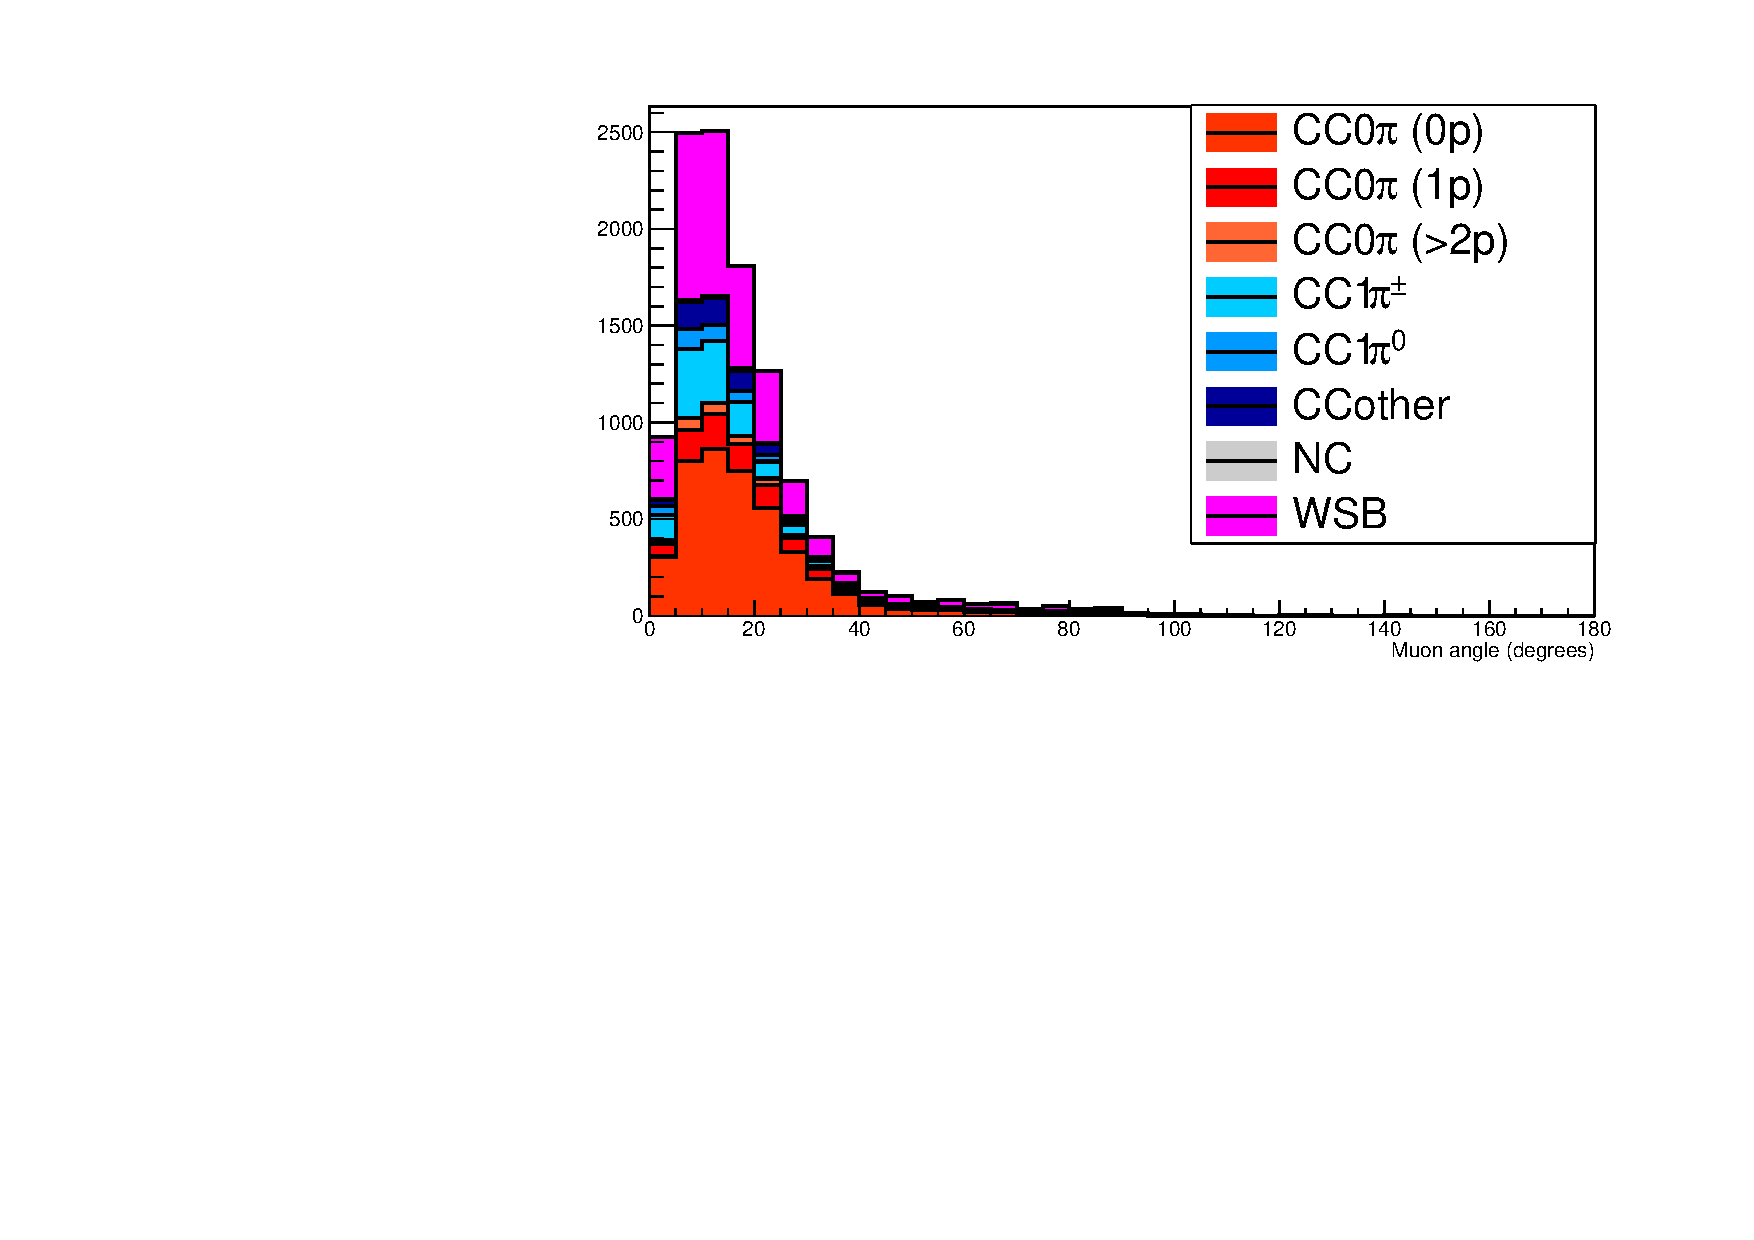
\includegraphics[width=0.55\linewidth, angle=270]{fig/RHCMuonAngle_StoppedOrThroughGoing.pdf}
%    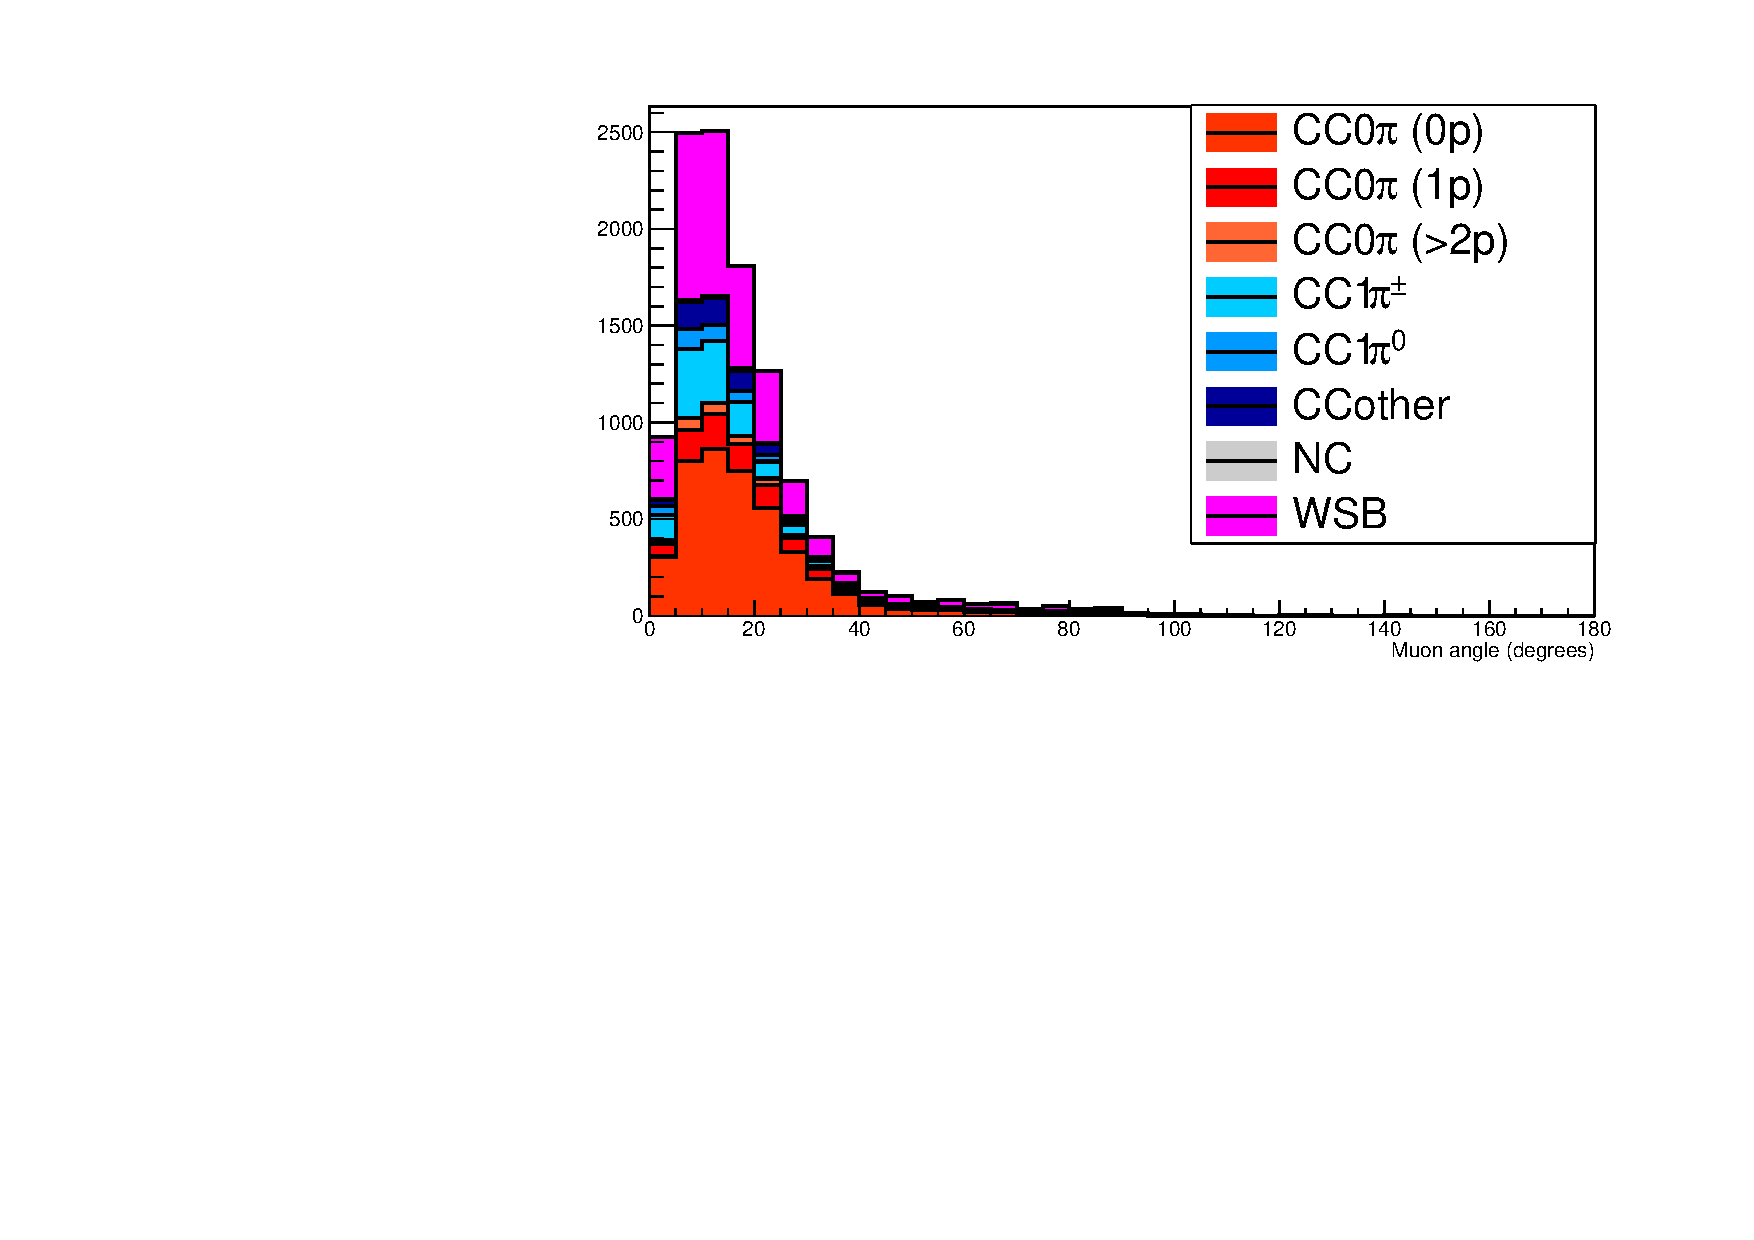
\includegraphics[width=\textwidth]{fig/RHCMuonAngle_StoppedOrThroughGoing.pdf}
    \end{subfigure}    
    \end{center}
  \caption{
The reconstructed angles of the longest tracks in the selected events in the neutrino-mode (left) and the antineutrino-mode (right).
}
\label{fig:angle_allcut}
\end{figure}
%
\begin{figure}[tbh]
 \begin{center}
  \begin{subfigure}{0.48\textwidth}
%     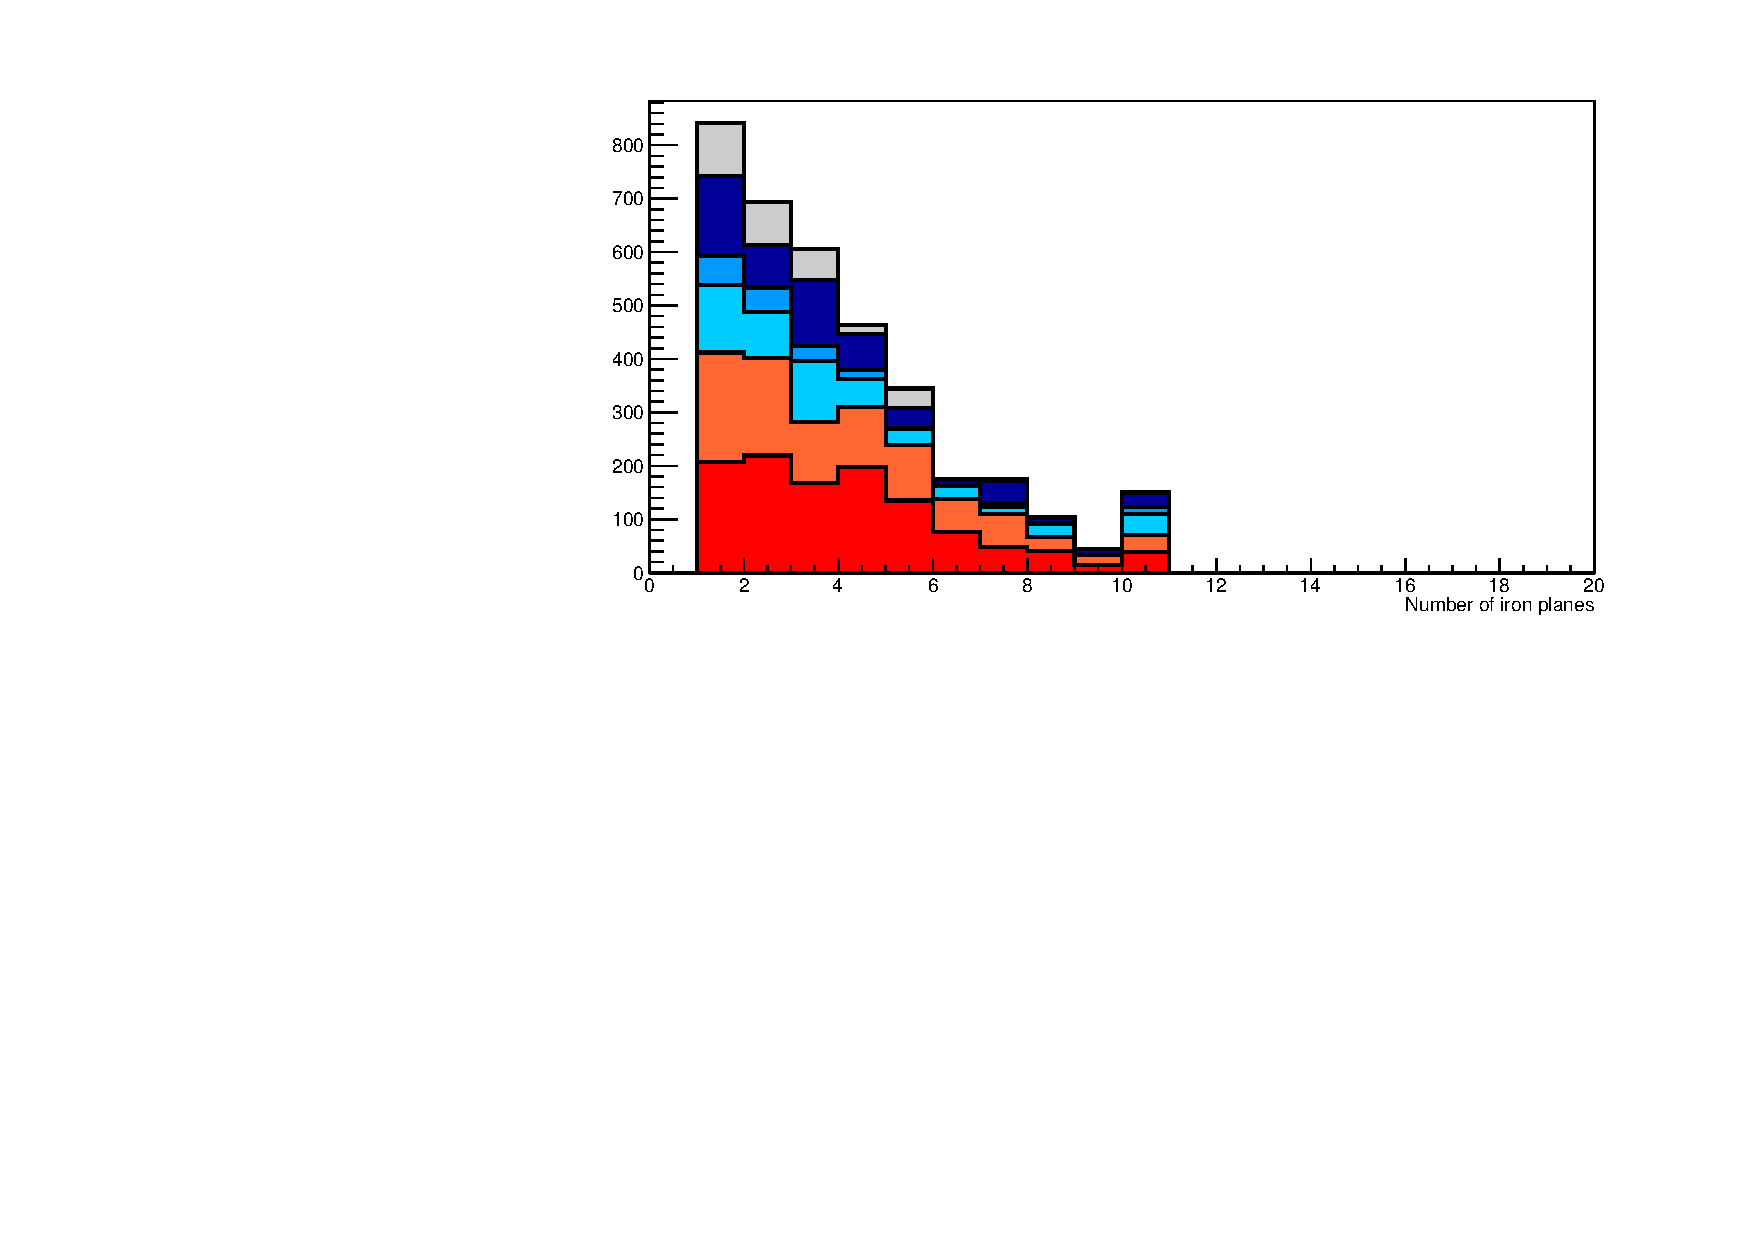
\includegraphics[width=\linewidth]{fig/FHCMuonPenetration_SideMRD_StoppedOrThroughGoing.pdf}
     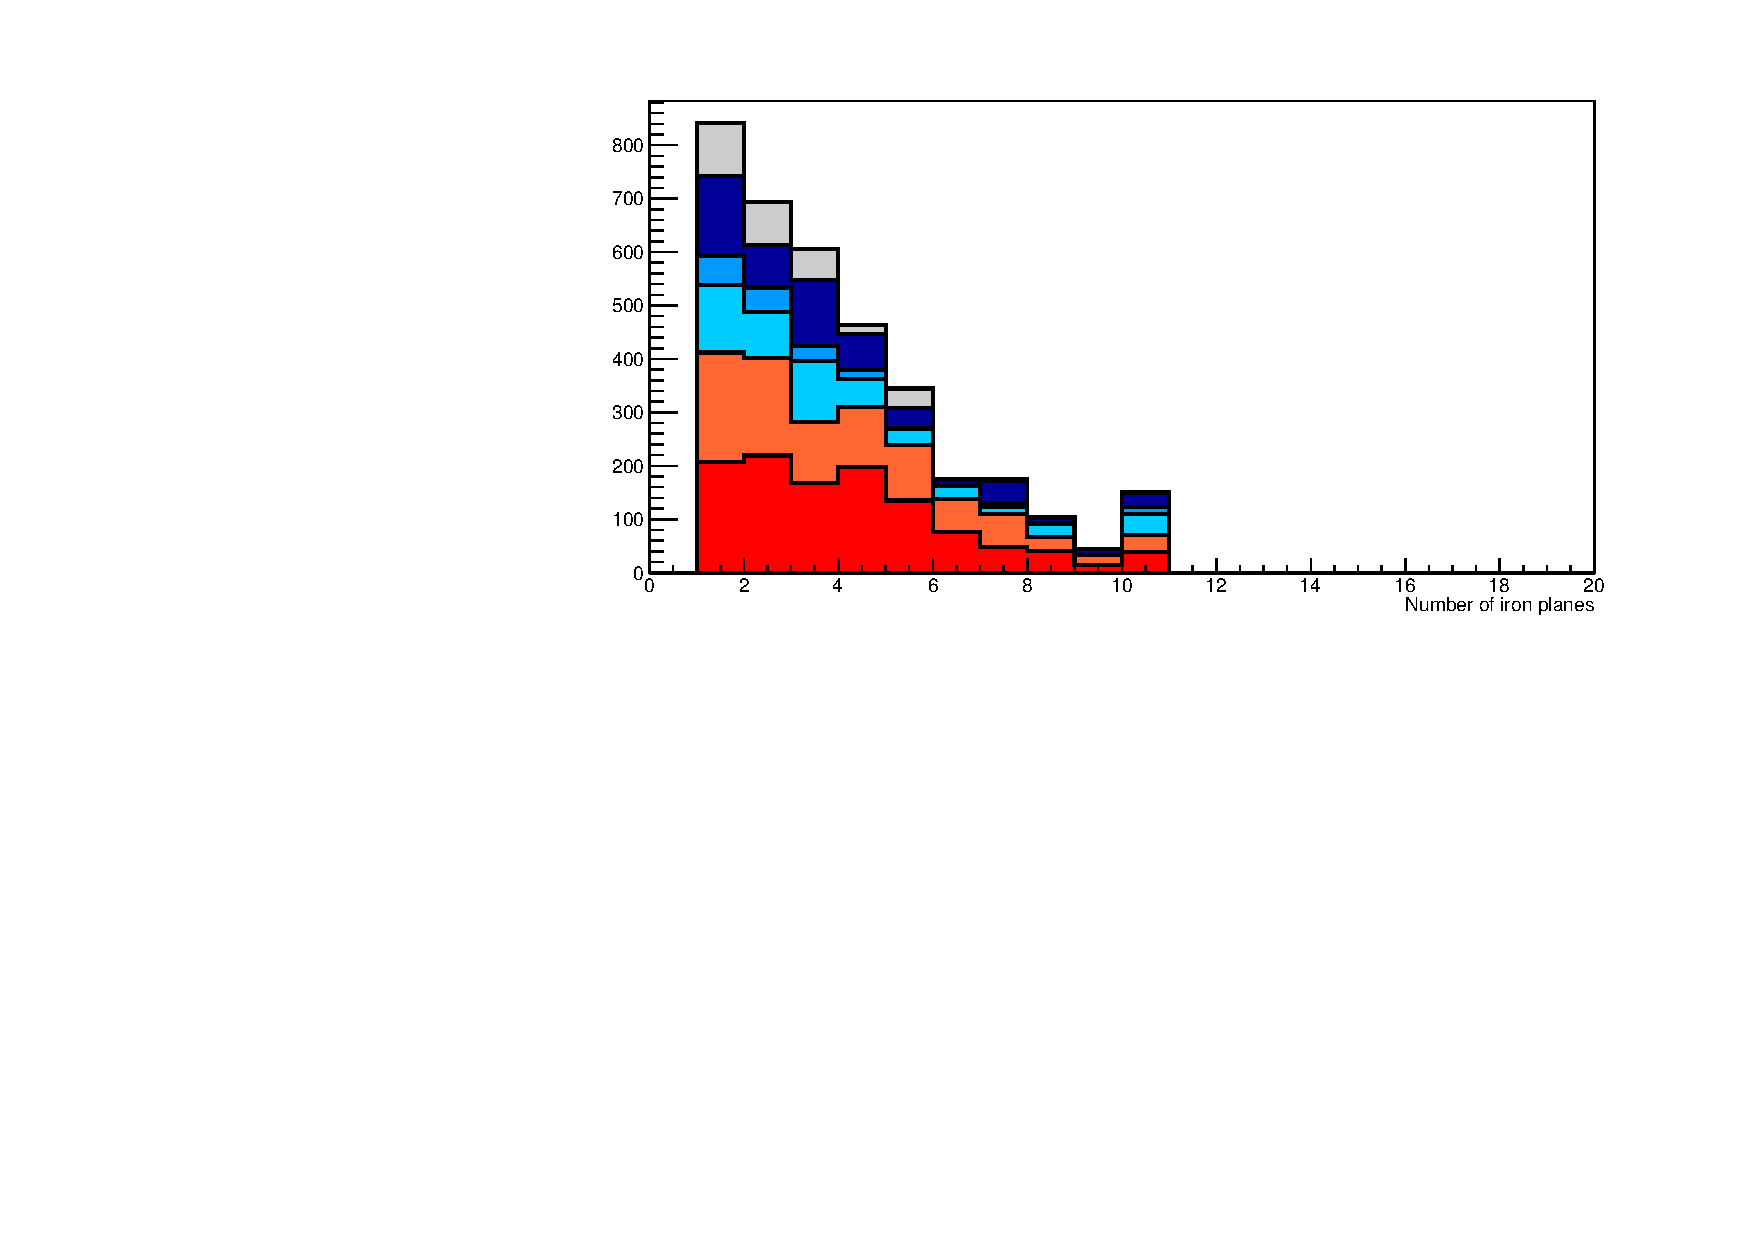
\includegraphics[width=0.55\linewidth, angle=270]{fig/FHCMuonPenetration_SideMRD_StoppedOrThroughGoing.pdf}
    \end{subfigure}
  \begin{subfigure}{0.48\textwidth}
%    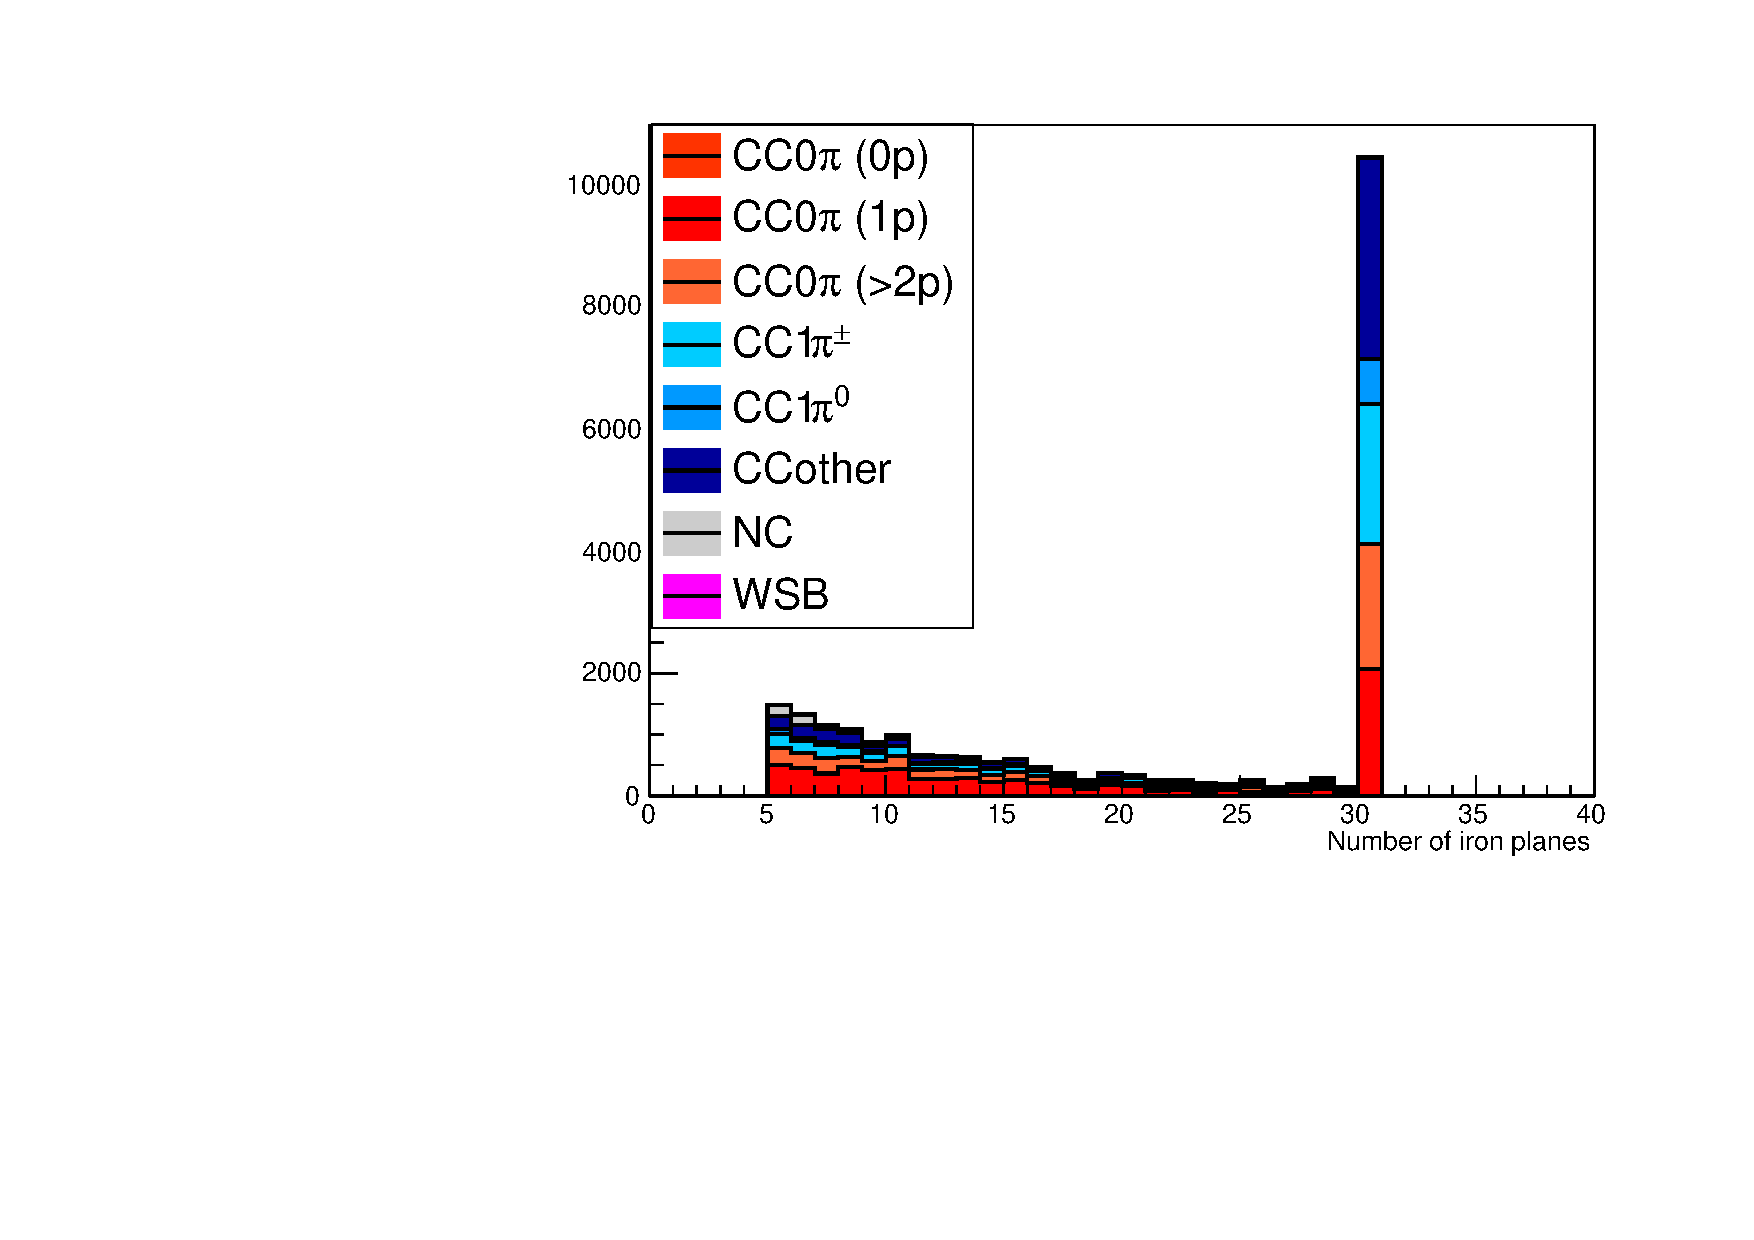
\includegraphics[width=\linewidth]{fig/FHCMuonPenetration_DownstreamMRD_StoppedOrThroughGoing.pdf}
    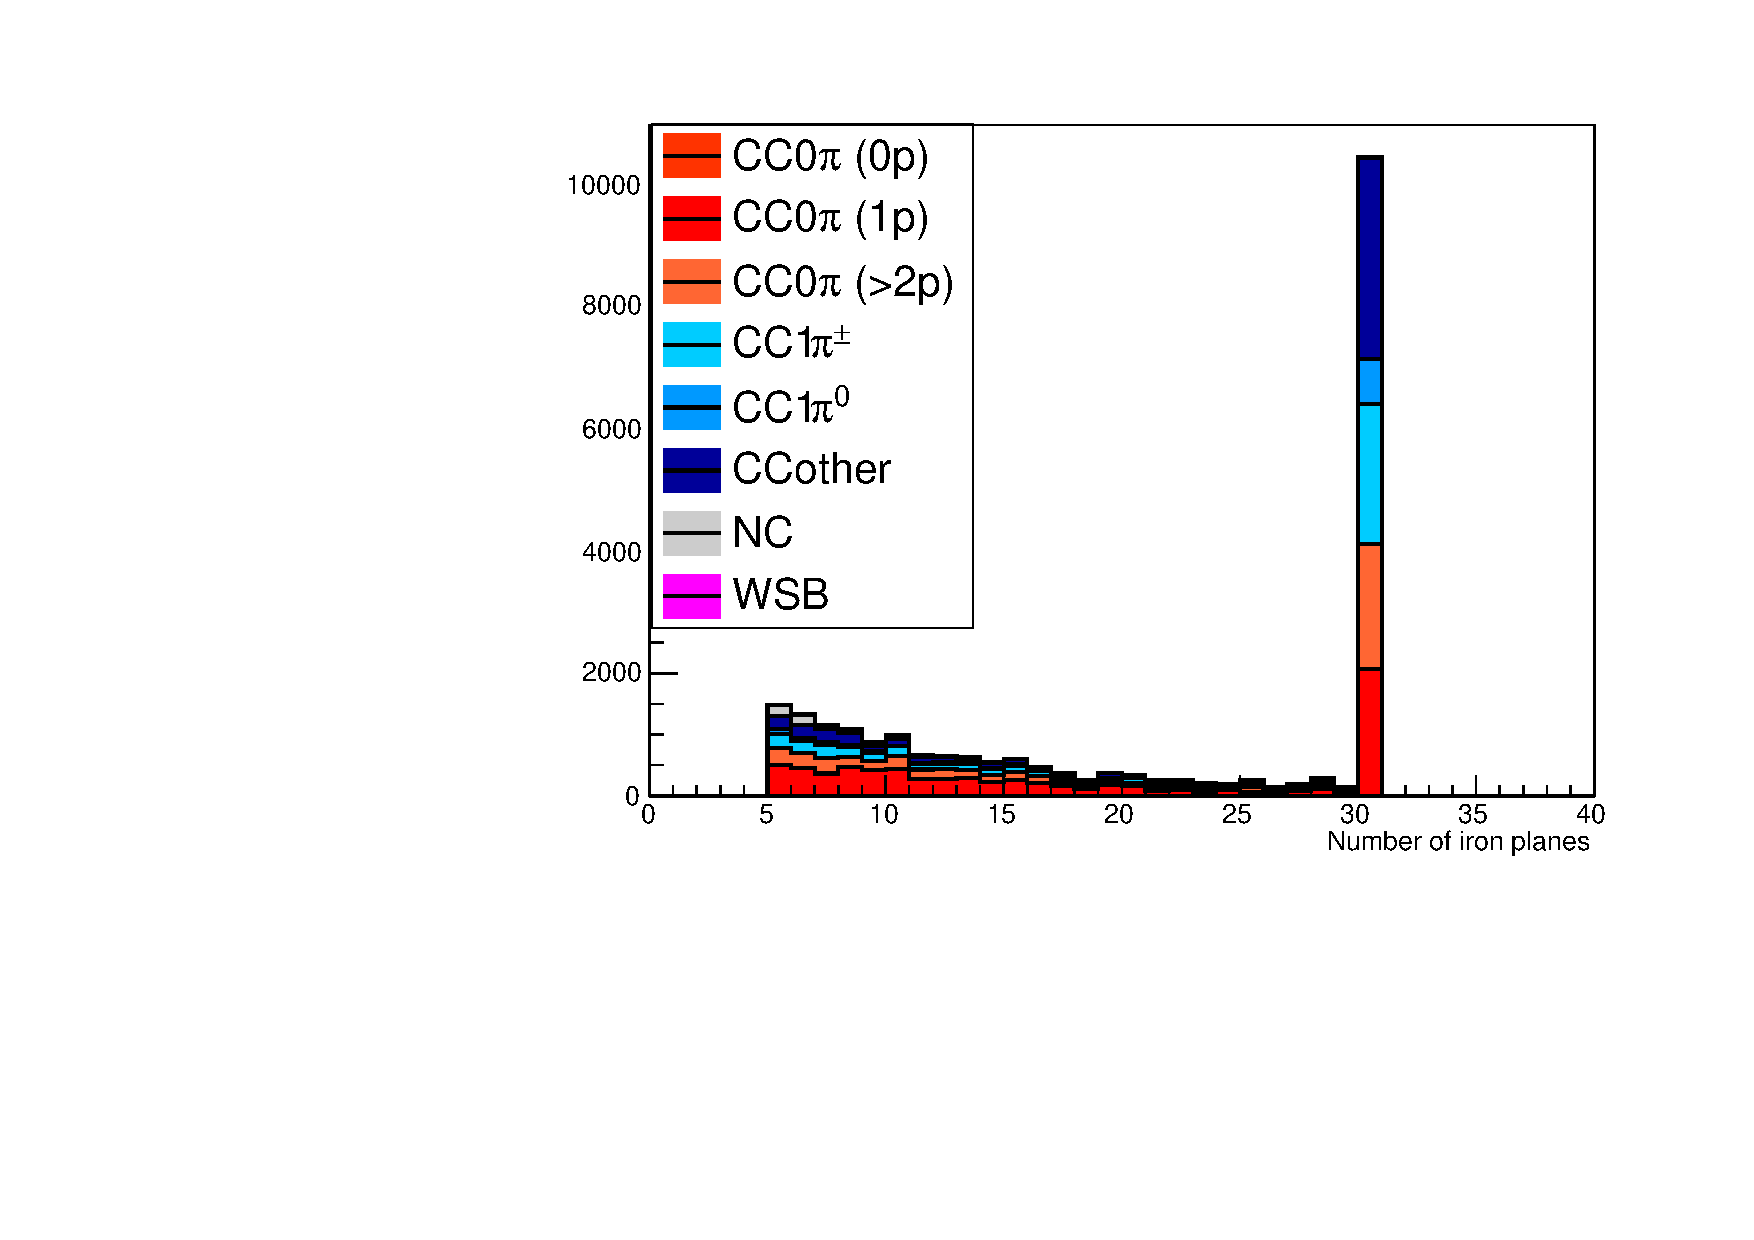
\includegraphics[width=0.55\linewidth, angle=270]{fig/FHCMuonPenetration_DownstreamMRD_StoppedOrThroughGoing.pdf}
    \end{subfigure}  
     \begin{subfigure}{0.48\textwidth}
%     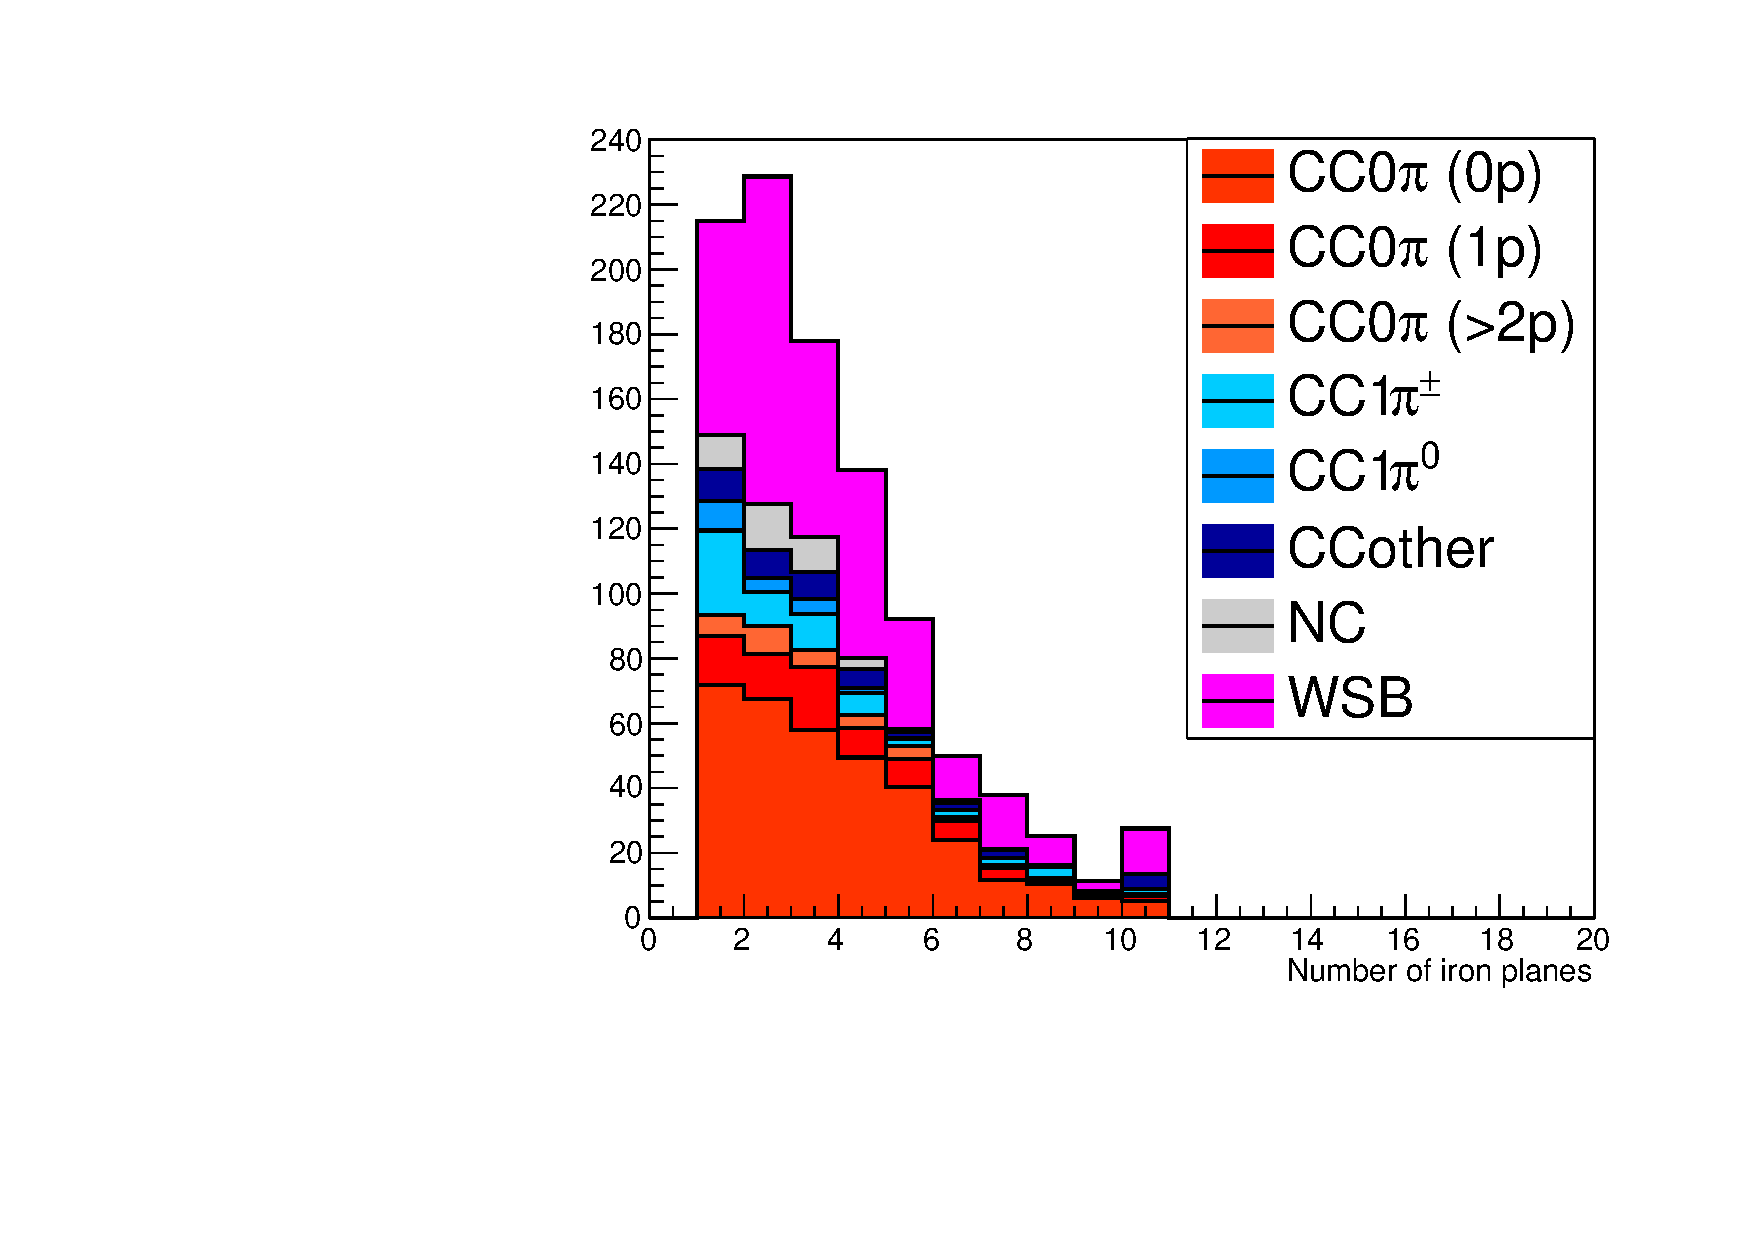
\includegraphics[width=\linewidth]{fig/RHCMuonPenetration_SideMRD_StoppedOrThroughGoing.pdf}
     \includegraphics[width=0.55\linewidth, angle=270]{fig/RHCMuonPenetration_SideMRD_StoppedOrThroughGoing.pdf}
    \end{subfigure}
  \begin{subfigure}{0.48\textwidth}
%    \includegraphics[width=\linewidth]{fig/RHCMuonPenetration_DownstreamMRD_StoppedOrThroughGoing.pdf}
    \includegraphics[width=0.55\linewidth, angle=270]{fig/RHCMuonPenetration_DownstreamMRD_StoppedOrThroughGoing.pdf}
    \end{subfigure}    
    \end{center}
  \caption{
Iron plane numbers in Side-MRD (left) and Baby-MIND (right) corresponding to the end points of the longest tracks in the selected events in the neutrino-mode (top) and the antineutrino-mode (bottom).
}
\label{fig:endpoint_longest_track}
\end{figure}



%Table \ref{tab:longest_track_particle} shows particles which produce the longest tracks in the selected events, and the fraction of muons is 85.6\%.
%
%\begin{table}[htb]
% \begin{center}
%   \caption{Particles which produce the longest tracks in the selected events.}
 %   \begin{tabular}{cc} \hline
 %     particles & fraction \\ \hline
 %     $\mu$ & 85.6\% \\
 %     $\pi^{+},\ \pi^{-}$ & 4.8\% \\
 %     p & 4.3\% \\
 %     e$^{+}$, e$^{-}$ & 4.5\% \\
 %     \hline
 %   \end{tabular}
 %   \label{tab:longest_track_particle}
 % \end{center}
% \end{table}

% Figure \ref{fig:eff_muon_angle_momentum_neutrino} shows detection efficiencies of muon tracks in the selected events as a function of muon's true angle and true momentum.
% The efficiency in the large angle region is low because Side-MRD modules only cover sides of the WAGASCI modules.
% The efficiency in the low momentum region is also low because more than two hits  are required to reconstruct the track in the WAGASCI detector.

% \begin{figure}[tbh]
%  \begin{center}
%   \begin{subfigure}{0.48\textwidth}
%     \includegraphics[width=\linewidth]{fig/eff_muon_angle_neutrino.pdf}
%    \end{subfigure}
%  \begin{subfigure}{0.48\textwidth}
%      \includegraphics[width=\linewidth]{fig/eff_muon_momentum_neutrino.pdf}
%    \end{subfigure}    
%    \end{center}
%  \caption{
%Detection efficiencies of muon tracks in the selected events as a function of muon's true angle (left) and true momentum (right).
%}
%\label{fig:eff_muon_angle_momentum_neutrino}
%\end{figure}



\subsection{Standalone WAGASCI-module tracking performance}
\label{sec:mc_study_standalone}

The previous section has described the inclusive charged-current event selection using the Muon Range detectors.
A muon is identified by requiring one track to penetrate multiple planes of the MRD's.
For the WAGASCI configuration described in Sec.~\ref{sec:mc_setup}, only $7\%$ of the muons are stopped in one of the WAGASCI modules. 
This proportion increases to $53\%$ for pions and $73\%$ for protons produced by neutrino interactions.% at $1.5^{\circ}$ off-axis. 
Figure~\ref{fig:stoppedproportions} shows the momentum distribution of these daughter particles as well as for the sub-sample stopped in one of the WAGASCI modules. 
For the measurement of the neutrino interaction final states, tracks of charged pions, protons and  low-momentum ($p_{\mu} < 300~$MeV/c) muons have to be reconstructed by the WAGASCI module.
Therefore, the standalone tracking abilities of the WAGASCI module, especially momentum threshold,  is important for the exclusive interaction measurements.
%
\begin{figure}[tbhp]
  \centering
\includegraphics[width=.7\textwidth]{fig/StoppedProportionsMomentum.pdf}
\caption{\label{fig:stoppedproportions} Momentum distribution of particles in WAGASCI (plain) and corresponding distributions only for particles stopping in the WAGASCI module (dashed).}
\end{figure}
%

Here we present the result of the study based on an original study done for the T2K ND280 upgrade with some modifications.
Though the cell size is similar to the WAGASCI configuration, the external dimensions are different (1864 mm $\times$ 600 mm $\times$ 1300 mm).
We present the results which are less affected by the difference of the external dimensions.
%Whenever the results are presented with this external size and this parameter is likely to impact the result, it will be mentioned.\\

A simplified criteria , but representing conditions for the WAGASCI module tracking, are applied to evaluate the reconstruction performance of the WAGASCI module. 
The fiducial volume is chosen as the inner cube of the module which surfaces are  4 × scintillator space = 100 mm distant from the module external surfaces.
%The neutrino interactions are simulated using NEUT v5.3.2. The NEUT input neutrino flux is estimated using JnuBeam v13a and assuming the detector to be located at $1.5^{\circ}$ off-axis, as in Section~\ref{sec:mc_study}.
%Note that the event reconstruction efficiency as a function of true neutrino energy might be changed at 1.5$^{\circ}$, due for example to different $Q^{2}$ distributions. For this reason, one has to note that the reconstruction results might change slightly from  $2.5^{\circ}$ and $1.5^{\circ}$. To avoid a similar change on the particle-only reconstruction efficiencies, they will be presented as a function of variables that completely characterize the particle kinematic state, \textit{i.e.} its momentum and angle.
%Figure~\ref{fig:trueinteraction_particle} shows  the vertices distributions the vertex distributions of the daughter particles of neutrinos interacting one standard WAGASCI water-module.
%In this section, we will show the detector reconstruction and particle identification in this phase space, both for leptonic and hadronic particles.
%We will finally show an empty WAGASCI module can highly enhance the ability to constrain the neutrino interaction final state which is critical to reduce the corresponding uncertainties.
%
%\begin{figure}
%  \centering
%  \begin{subfigure}{.49\textwidth}
%    \includegraphics[width=\linewidth]{fig/TrueInteractions_Muon.pdf}
%  \end{subfigure}
%  \begin{subfigure}{.49\textwidth}
%    \includegraphics[width=\linewidth]{fig/TrueInteractions_Pion.pdf}
%  \end{subfigure}
%  \begin{subfigure}{.49\textwidth}
%    \includegraphics[width=\linewidth]{fig/TrueInteractions_Proton.pdf}
%  \end{subfigure}
%  \caption{\label{fig:trueinteraction_particle} True number of muons (left), charged pions (right) and protons (bottom) in the two WAGASCI water-module as a function of the particles momenta and angles at $1.5^{\circ}$.}
%\end{figure}
%
%\subsection{Reconstruction algorithm}
%\label{Sec:Reco}
%\subsubsection{Description}
%For this section, an ideal ``simulated'' reconstruction is developed.
A track is reconstructed if:
%\begin{enumerate}
%\item The particle is charged.
%\item Has at least one hit (energy deposit $> 2.5$ photo-electron) in a scintillator.\\
%\item The particle enters one TCP and has one hit in the tracker.\\
%  Or\\
\begin{itemize}
\item The track is long enough and has at least 2 hits in both of two views (XZ, YZ).
  In the pure longitudinal or transverse going tracks, it corresponds to the track length of $100~$mm.
\item The track shall not be superimposed with longer tracks in both of two views. The superposition criterion is estimated with the distance inter-tracks (DIT) which corresponds to the orthogonal distance between two tracks at the ending point of the shortest one (see Figure~\ref{fig:DIT}). 
%For a track we call track 1, the super position criterion is tested with every longer track that
% every longer tracks that 
%starts at the same vertex. Let $\vec{p_{1}}$ the vector of track 1, and $p_{1}^{a}$ its projections in the XZ, YZ and XY planes respectively for i=1,2,3. Note that these are 
%projections onto 2D planes and not onto a direction vector.
% projections in a 2D planes and not on a direction vector. 
%this case, the relative angle between track 1 and a longer track, track 2, (of vector 
% In this case, the relative angle between the track 1 and a longer track 2 (of vector 
%$\vec{p_{2}}$) in a view a is given by:
%\begin{equation}
%  \cos \theta = \frac{\vec{p_{1}^{a}} \cdot \vec{p_{2}^{a}}}{||\vec{p_{1}^{a}}|| ||\vec{p_{2}^{a}}||} 
%\end{equation}
%and the distance inter track is given by:
%\begin{equation}
%  \text{DIT} = ||\vec{p_{1}^{a}}|| \sin \theta
%\end{equation}
The DIT should be higher than $4 \times \text{scintillator width}$ (=100~mm) for the shorter track not to be superimposed with the longer track.
\end{itemize} 
%\end{enumerate}
\begin{figure}[htbp]
  \centering
  \includegraphics[width=.7\textwidth]{fig/DistanceInterTracks.pdf}
  \caption{\label{fig:DIT} Definition of the distance inter tracks.}
\end{figure}

\subsubsection{Expected performance of the water-in WAGASCI module}
\label{sec:mc_waterin}
Figures~\ref{fig:efficiency_particle} shows the expected track reconstruction efficiency obtained with the criteria above.
Table~\ref{tab:reconstructedparticles} summarizes the reconstruction efficiencies and the reconstruction momentum thresholds.
This threshold is defined as the momentum under which the reconstruction efficiency falls under $30\%$.
The thresholds for muon and pion are $150~$MeV/c. %Most of the muons are above this threshold (see Figure~\ref{fig:trueinteraction_particle}) which leads to a $79\%$ reconstruction efficiency. 
\begin{table}[htbp]
% \small
  \begin{center}
    \caption{\label{tab:reconstructedparticles} Reconstruction efficiency and momentum threshold for muons, pions and protons.
The threshold is defined as the momentum under which the reconstruction efficiency falls under $30\%$.}
    \begin{tabular}{c|ccc}
      \hline
      & $\mu$ & $\pi$ & p \\
      \hline
      Reconstruction Efficiency & 79\% & 52\% & 26\% \\\hline
%      Purity & 56\% & 14\% & 31\% \\
      Momentum threshold & 150 MeV/c & 150 MeV/c & 550 MeV/c \\
      \hline
    \end{tabular}
  \end{center}
\end{table}
The lower pion and proton efficiencies (respectively $52\%$ and $26\%$) are due to lower momentum and also due to the secondary interaction.
Efficiencies of each particle type tend to decrease in the backward region due to lower particle momenta.
However, for a fixed momentum value, the reconstruction efficiency do not strongly depend on the angle thanks to the WAGASCI grid structure. 
\begin{figure}[htbp]
  \centering
    \begin{subfigure}{.49\textwidth}
    \includegraphics[width=\linewidth]{fig/Efficiency_Muon.pdf}
  \end{subfigure}
    \begin{subfigure}{.49\textwidth}
    \includegraphics[width=\linewidth]{fig/Efficiency_Pion.pdf}
  \end{subfigure}
    \begin{subfigure}{.49\textwidth}
    \includegraphics[width=\linewidth]{fig/Efficiency_Proton.pdf}
  \end{subfigure}
  \caption{\label{fig:efficiency_particle} Reconstruction efficiency of muons (left), charged pions (right) and protons (bottom) in the WAGASCI water-module as a function of the particles momenta and angles.}
\end{figure}

%The reconstruction is thereafter tested on neutrino events. Table~\ref{tab:reconstructedinteractions} summarizes the number of reconstructed events and efficiencies for each interaction type. As expected from the high muon reconstruction efficiency, the charged current interactions have reconstruction efficiencies $\geq 85\%$.
%\begin{table}[htbp]
%  \small
%  \begin{center}
%    \begin{tabular}{|c|c|c|c|c|c|}
%      \hline
%      \hline
%      & CC0$\pi$ & CC1$\pi$ & CCOthers & NC & All \\
%      \hline
%      Reconstruction efficiency & 85\% & 87\% & 91\% & 22\% & 68\% \\
%      \hline
%      \hline
%    \end{tabular}
%    \caption{\label{tab:reconstructedinteractions} Number of true interactions reconstructed. The purity and reconstruction efficiency of each true interaction is also shown.}
%  \end{center}
%\end{table}
%
%The reconstruction efficiencies as a function of the neutrino energy and muon kinematics are respectively shown on Figure~\ref{fig:efficiency_enu} and \ref{fig:efficiency_muonkinematics}.
%\begin{figure}
%  \centering
%\includegraphics[width=.7\textwidth]{fig/Efficiency_Enu.pdf}
%  \caption{\label{fig:efficiency_enu} Reconstruction efficiency of all neutrino (black), CC (red) and NC (blue) interactions in the WAGASCI water-mod%ule as a function of the neutrino energy.}
%\end{figure}
%\begin{figure}
%  \centering
%\includegraphics[width=.7\textwidth]{fig/Efficiency_MuonKinematics.pdf}
%  \caption{\label{fig:efficiency_muonkinematics} Reconstruction efficiency of CC interactions in the WAGASCI water-module as a function of the muon kinematic variables (momentum and angle).}
%\end{figure}
%\clearpage

%Note that a Particle Identification Algorithm has been also developed. It is based on the charge deposition of the particles in the scintillator, of the detection of a decay-electron. 
%However, information depends highly on the number of scintillator hits by a particle,
% this information highly depends on the number of scintillator hit by a particle, 
%which creates an important difference between a real WAGASCI module and the one used for the ND280-upgrade simulation. For this reason, the corresponding results will not be detailed here, but can be found in~\cite{ND280Upgrade}.

\subsubsection{Expected performance of the water-out WAGASCI module}
One experimental option is to remove water from one of the two WAGASCI modules.
%In the nominal configuration, $20\%$ of the neutrino interactions occurs on scintillators (C$_{8}$H$_{8}$).
%This background should be removed in order to measure the neutrino interaction on the same target as Super-K, which suppress the differences in cross-section models.
%For this purpose, we propose to use a water-out module, where the water is replaced by air.
The detector is fully active and has a $3~$mm spatial resolution (scintillator thickness) which create and ideal detector to reconstruct and identify hadrons, and study 2p2h interaction.
%The counter-part is the difference in particle energy deposition between the water and this water-out module that will need to be corrected for.
%In this section, we present the capabilities of such a module, and the impact it can have on cross-section measurements for the neutrino community in genral and T2K in particular.\\
The same reconstruction criteria as in Sec.~\ref{sec:mc_waterin} are applied for the water-out module.
Figure~\ref{fig:reconstructionefficiencyparticle_mometum} shows the comparison between the water-in and the water-out reconstruction efficiencies for muon, pions and protons.
$90\%$ of the muons and $87\%$ of the pions are reconstructed, while $70\%$ of the protons are even reconstructed.
It allows to low down the proton threshold to 250~MeV/c (see Table~\ref{tab:reconstructedparticles_empty}).     
%Number of interactions: true, reconstructed, selected.
%Efficiency particle per particle.
%Efficiency interaction per interaction
\begin{figure}[htbp]
  \centering
    \begin{subfigure}{.49\textwidth}
      \includegraphics[width=\linewidth]{fig/EfficiencyParticles_Momentum.pdf}
    \end{subfigure}
    \begin{subfigure}{.49\textwidth}
      \includegraphics[width=\linewidth]{fig/EfficiencyParticles_Momentum_Empty.pdf}
    \end{subfigure}
  \caption{\label{fig:reconstructionefficiencyparticle_mometum} Reconstruction efficiency for muons, pions and protons in the water-in (left) and water-out (right) modules.}
\end{figure}
%
\begin{table}[htbp]
% \small
  \begin{center}
    \caption{\label{tab:reconstructedparticles_empty} Reconstruction efficiency, proportions of $\mu$-like and non $\mu$-like and momentum threshold for muons, pions and protons for the water-out module.
The threshold is defined as the momentum under which the reconstruction efficiency falls under $30\%$.}
    \begin{tabular}{c|ccc}
      \hline
      & $\mu$ & $\pi$ & p \\
      \hline
      Reconstruction Efficiency & 90\% & 87\% & 70\% \\ \hline
 %     Reconstruction Purity & 37\% & 13\% & 49\% \\
      Momentum threshold & 50 MeV/c & 50 MeV/c & 250 MeV/c  \\ \hline
    \end{tabular}
  \end{center}
\end{table}
%
%As a consequence of tracking even low momenta particle, the reconstruction efficiency is uniform and almost maximal on the entire $\cos \theta_{\mu}$ phase space, as shown on Figure~\ref{fig:efficiency_muonkinematics_empty}.
%Since the fiducial mass represents 0.25~tons, the total number of events is divided by a factor of 3 compared to the water-in module.
The water-out module offers interesting possibilities to study 2p2h interaction since $70\%$ of the protons are reconstructed.
%In the future, a possible separation as a function of the number of proton track will be studied. Morevover, we are currenly pursuing the use of single and double transverse variables (cite Xianguo) to open new possibilities for separating np-nh from Final State Interactions, or for isolating the interactions on hydrogen from interactions on carbon in this module. 
%CHekc the proportions of stopped in 1cm3 cell and water-out

%\begin{figure}
%  \centering
%\includegraphics[width=.7\textwidth]{fig/Efficiency_MuonKinematics_Empty.pdf}
%  \caption{\label{fig:efficiency_muonkinematics_empty} Reconstruction efficiency of CC interactions in the WAGASCI empty module as a function of the muon kinematic variables (momentum and angle).}
%\end{figure}

%\section{Group organization}

\section{Schedule}
We would like to start a physics data taking from T2K beam time after the summer shutdown in 2018.
By then, commissioning and tests of the detectors will be completed in J-PARC T59.
The experiment can run parasitically with T2K, therefore we request no dedicated beam time nor beam condition as discussed in the following section.

%Once the approved POT is accumulated, the WAGASCI modules will be removed from the experimental site, but we would like to keep the Baby-MIND and the Side-MRD modules on the B2 floor of the NM pit as common platforms of future neutrino experiments using the T2K neutrino beam.

\section{Requests}

\subsection{Neutrino beam}
The experiment can run parasitically with T2K, therefore we request no dedicated beam time nor beam condition.
As data taking periods, we request the `nominal' T2K one-year operation both for the neutrino beam and the antineutrino beam.
The T2K has been requesting $0.9\times10^{21}$~POT/year and actually accumulating about $0.7\times10^{21}$~POT/year in recent years.
For each year, starting from the Autumn,  T2K is running predominantly in the neutrino mode or in the antineutrino mode.
Our request is to have one-year neutrino-mode data and another one-year antineutrino mode data
assuming that the POT for the fast extraction in each year is more than $0.5\times10^{21}$~POT.

\subsection{Equipment request including power line}
We request the followings in terms of equipment on the B2 floor:
\begin{itemize}
\item {Site for the WAGASCI modules, Side-MRD modules and BabyMIND and their electronics system on the B2 floor of the near detector hall (Figure \ref{fig:all_detector_topview} and \ref{fig:location}).}
\item {Anchor points (holes) on the B2 floor to secure the WAGASCI modules, Side-MRD module and Baby-MIND, detailed floor plans to be communicated in a separate document.}
\item {Power line for the magnets in Baby-MIND: 400 V tri-phase 48-to-62 Hz, capable of delivering 12 kW. We have a wish for the magnet power line to be installed and available to us by beginning of March 2018.}
\item Electricity for electronics and water circulation system, 3 kW, standard Japanese electrical sockets.
	\begin{enumerate}
		\item Online PCs: 2.1 kW
		\item Electronics: 0.7 kW
		\item Water sensors: 1 kW
	\end{enumerate}
\item Air conditioner for cooling heat generation at Baby-MIND magnets, online PCs and electoronics
\item Beam timing signal and spill information
\item Network connection
\end{itemize}

The infrastructure for much of the above exists already.
Exceptions are the power line for the magnet and the electronics and holes in the B2 floor to anchor the detector support structures.

After this WAGASCI experiment, Baby MIND and Side-MRD's will remain if approved by J-PARC, and be used as common platforms of future neutrino experiments using the J-PARC neutrino beam.

\section{Conclusion}


\bibliographystyle{plain}
\bibliography{wagasci}

\end{document}  
